%============================================================================
\chapter{Higher Order and TVD Schemes}\label{chap:higher-order-schemes}
%============================================================================


Higher order schemes, i.e. schemes whose accuracy scales with cell spacings $\Delta x$ and time
step sized $\Delta t$ with a power greater than $1$, are very desirable for practical applications.
While they require more calculations for a single cell update $\uc^{n+1}_i$, their improved scaling
makes them attractive since increasing the resolution, i.e. reducing $\Delta x$ and $\Delta t$,
leads to improved results. There is always a turning point at which the additional computational
cost per update is overtaken by the better scaling, leading to more accurate solutions at a
comparatively lower computational cost. For example, say a second order accurate solution
$\uc_{2}^{n+1}$ requires 4 times more computations in order to be second order accurate, i.e. scale
with $\Delta x^2$, compared to the first order solution $\uc_{1}^{n+1}$. If $N$ is the number of
computations required to obtain the full solution $\uc_{1}^{n+1}$ for all cells, then decreasing
$\Delta x$ by a factor of $8$ means also increasing the number of required cells to cover the same
volume. The computational cost of the first order method increases linearly to $8N$, and the error
will be reduced by a factor of $1/8$. For the second order scheme, the initial cost would be $4 N$,
and the cost after reducing $\Delta x$ by a factor of $8$ increases linearly to $32 N$. However the
error is reduced by a factor $\propto \Delta x^2$, i.e. by a factor of $1/64$. In order to obtain
this sort of improvement of accuracy using the first order accurate scheme, we'd need to decrease
$\Delta x$ by a factor of $64$, leading to a required computation workload of $64 N$, or twice as
much as the second order scheme. Additionally, the first order scheme would have much higher memory
requirements in order to reproduce the same accuracy, as it would need to store $8$ times more
cells.\footnote{The factor 8 stems from the assumption that the problem is one dimensional, and
that the number of cells is directly proportional to the cell size $\Delta x$. For two and three
dimensions and assuming cells of equal size, an additional factor of $8$ needs to be added
for each additional dimension. This leads to $64$ and $512$ more cells required to be stored,
respectively.}


Extending Godunov's method to higher order accuracy can at first glance seem straightforward. In
this chapter, two distinct approaches to do so are discussed:

\begin{itemize}
\item A method that relaxes the assumption that the states inside a cell are piece-wise constant,
and instead assumes that they are piece-wise linear, called the MUSCL-Hancock method
\item A method that attempts to find an improved expression for the inter-cell fluxes $\F_{i\pm
\half}$ by relaxing the assumption that the states left and right of the boundary remain constant
throughout the entire time step, called the Weighted Average Flux (WAF) method.
\end{itemize}


However, higher order accurate methods come with a plethora of new problems that weren't present
for first order methods. In particular, if left untreated, second order methods will always develop
spurious oscillations in the solutions, which typically are violently unstable. There are ways to
handle this issue, namely by applying slope and flux limiters, but the way they work can sometimes
appear like witchcraft. To showcase the problems of second order methods and how the limiters work,
we first have a look at second order schemes for the ol' reliable linear advection with constant
coefficients.



%=======================================================
\section{Higher Order Schemes For Scalar Equations}
%=======================================================



%=======================================================
\subsection{The WAF Scheme}\label{chap:WAF}
%=======================================================

The core idea of the Weighted Average Flux (WAF) scheme is to improve the estimate for the fluxes
at the cell boundaries, $\F_{i \pm \half}$.
When deriving Godunov's method, we started off by using the integral form of the conservation law.
A key part of solving the integral of the fluxes over time was to make use of the fact that
solution to the Riemann problem centered between two adjacent cells, $\uc_i^n$ and $\uc_{i+1}^n$,
predicts that for all $t > 0$ the solution at the boundary will remain constant.
The general solution structure of the Riemann problem consists of waves that will emanate from the
center and travel along characteristics, as is shown in e.g.
Figures~\ref{fig:riemann-linear-hyperbolic-system} and \ref{fig:riemann-solution}. However, given
that the states are represented as integral averages of continuous states, i.e.

\begin{align}
    \uc_i^n = \frac{1}{\Delta x} \int\limits_{x_{i-\half}}^{x_{i+\half}} \uc(x, t^n) \de x
\end{align}

a consequence of waves emanating from cell boundaries and propagating through the cells is that the
integral averaged cell states won't be constant for $t > t^n$ precisely \emph{because} there are
waves propagating through them.
The WAF method tries to get a better estimate of the fluxes that would actually pass between
a boundary if the underlying problem weren't discretized, but continuous. To do so, the constant
fluxes $\fc_{i + \half}$ of Godunov's scheme are replaced by fluxes averaged over space.
Explicitly, the fluxes are estimated at the midpoint in time between two time steps, $t^{n+\half} =
t^n + \frac{1}{2} \Delta t$, and averaged from the center of the left cell, $x_i$, to the center of
the right cell, $x_{i+1}$:

\begin{align}
    \fc_{i+\half}^{WAF} = \frac{1}{\Delta x} \int\limits_{x_i}^{x_{i+1}} \fc(\uc_{i+\half}(
t^{n+\half})) \de x
\end{align}

$\uc_{i+\half}$ is the solution to the Riemann problem with initial data $\uc_i$ and $\uc_{i+1}$.
Figure~\ref{fig:advection-WAF} illustrates the situation assuming a positive coefficient $a > 0$.
Making use of the analytical solution of the Riemann problem,

\begin{align}
    \uc(x, t) = \begin{cases}
                 \uc_i & \text{ if } \frac{x - x_{i-\half}}{t} < a \\
                 \uc_{i+1} & \text{ if } \frac{x - x_{i-\half}}{t} > a
                \end{cases}
\end{align}





\begin{figure}
    \centering
    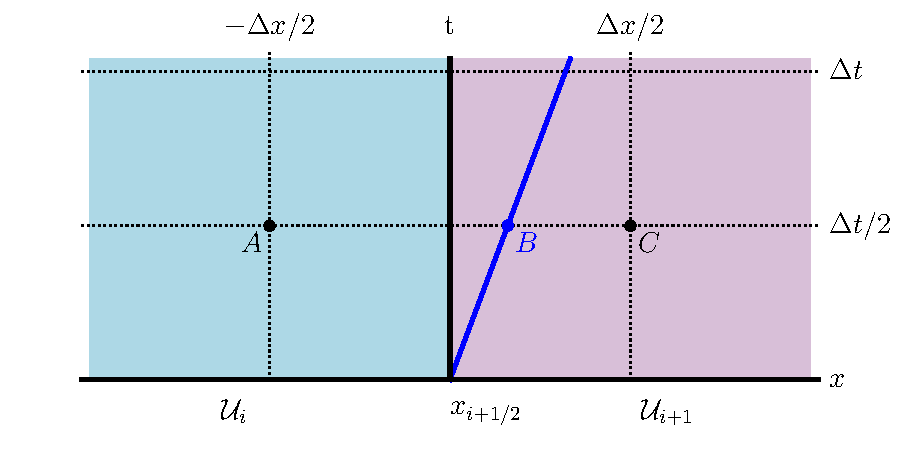
\includegraphics[width=.8\textwidth]{./figures/FV/WAF.pdf}%
    \caption[WAF flux estimate for linear advection]{
The set-up for computing the WAF inter-cell flux at the mid-step in time. For $t > 0$ and a
coefficient $a > 0$, the emanating wave (blue line) will intersect the $t = \Delta t/2$ line at
some point $B > x_{i+\half}$
    }
    \label{fig:advection-WAF}
\end{figure}





we can subdivide the interval $[x_i, x_{i+1}]$ into two subdomains along the $t = t^{n + \half}$
line in Figure~\ref{fig:advection-WAF}: Let point $A$ be at $(x_i, t^{n+\half})$, point $C$ at
$(x_{i+1}, t^{n+\half})$, and point $B$ at the position of the discontinuity, $(x_{i+\half}+a
\Delta t / 2, t^{n+\half})$. The lengths of the subdomains $\overline{AB}$ and $\overline{BC}$ are
given by
\begin{align}
    \overline{AB} &= \frac{\Delta x}{2} + a \frac{\Delta t}{2}
        = \frac{1}{2}\left(1 + \frac{a \Delta t}{\Delta x}\right) \Delta x
        = \frac{1}{2}\left(1 + C_{CFL} \right) \Delta x  \\
    \overline{BC} &= \frac{\Delta x}{2} - a \frac{\Delta t}{2}
        = \frac{1}{2}\left(1 - C_{CFL} \right) \Delta x
\end{align}


Since the states between
$\overline{AB}$ and $\overline{BC}$ are constant, the integral averaged flux is trivial to compute:

\begin{align}
\fc_{i+\half}^{WAF}
    &= \frac{1}{\Delta x} \int\limits_{x_i}^{x_{i+1}} \fc(\uc_{i+\half}( t^{n+\half})) \de x \\
    &= \frac{1}{\Delta x} \left[
    \int\limits_{A}^{B} \fc(\uc_{i+\half}^{n+\half}) \de x +
    \int\limits_{B}^{C} \fc(\uc_{i+\half}^{n+\half}) \de x
    \right] \\
    &= \frac{1}{\Delta x} \left[
    \overline{AB} \fc(\uc_{i+\half}^{n+\half}) |_{x = A}^B +
    \overline{BC} \fc(\uc_{i+\half}^{n+\half}) |_{x = B}^C
    \right] \\
    &= \frac{1}{\Delta x} \left[
    \overline{AB} (a \uc_i) + \overline{BC} (a \uc_{i+1})
    \right] \\
    &= \frac{1}{\Delta x} \left[
        \frac{1}{2}\left(1 + C_{CFL} \right) \Delta x (a \uc_i) +
        \frac{1}{2}\left(1 - C_{CFL} \right) \Delta x  (a \uc_{i+1})
    \right] \\
    &=  \frac{1}{2}\left(1 + C_{CFL} \right) (a \uc_i) +
        \frac{1}{2}\left(1 - C_{CFL} \right) (a \uc_{i+1}) \label{eq:WAF-flux}
\end{align}

For $a > 0$, the flux is a weighted average of the upwind flux $\fc_i = a \uc_i$ and the downwind
flux $\fc_{i+1} = a \uc_{i+1}$, hence the name of the method.

The final update scheme reads as follows:

\begin{align}
    \uc_{i}^{n+1} =
        \uc_i + \frac{\Delta t}{\Delta x}\left(\fc_{i-\half}^{WAF} - \fc_{i+\half}^{WAF} \right)
\end{align}

Formally, this equation looks identical to Godunov's method, given in eq.~\ref{eq:godunov-scheme}.
The big difference which results in a higher order accuracy is ``hidden'' in the expression for the
fluxes $\fc^{WAF}_{i\pm \half}$. They are now estimated using an integral average of cell states
which are no longer assumed to remain constant during a time step $\Delta t$, but are allowed to
change over the duration thereof.






%=======================================================
\subsection{The MUSCL-Hancock Scheme}\label{chap:MUSCL-Hancock}
%=======================================================


The approach behind MUSCL (Monotone Upstream-Centered Schemes for Conservation Laws) schemes to
achieve higher order accuracy is to depart from the piece-wise constant reconstruction of the data,
and use a higher order interpolation instead. The simplest way of modifying the piece-wise constant
data is to replace the constant states $\uc_i^n$ with a linear local reconstruction

\begin{align}
    \uc_i^n(x) = \uc_i^n + (x - x_i) s_i, \quad x \in [0, \Delta x]
\end{align}

where $s_i$ is a suitably chosen slope of $\uc_i(x)$. The integral average of $\uc_i^n(x)$ in each
cell is identical to the piece-wise constant state, and hence the reconstruction remains
conservative. A general way of defining a slope is using a free parameter $\omega \in [-1, 1]$ and
write

\begin{align}
    s_i = \frac{1}{\Delta x} \left[
    \frac{1}{2} ( 1 + \omega ) (\uc_{i}^n - \uc_{i-1}^n) +
    \frac{1}{2} (1 - \omega)(\uc_{i+1}^n - \uc_{i}^n)
    \right]
\end{align}

Some special values for $\omega$ are:
\begin{align}
    \omega = 0: && \text{Centered slope (Fromm) } &&
        &s_i^n = \frac{\uc_{i+1}^n - \uc_{i-1}^n}{ 2
\Delta x}\\
    \omega = 1: && \text{Upwind slope (Beam-Warming) } &&
        &s_i^n = \frac{\uc_{i}^n - \uc_{i-1}^n}{\Delta x} \\
    \omega = -1: && \text{Downwind slope (Lax-Wendroff) } &&
        &s_i^n = \frac{\uc_{i+1}^n -
\uc_{i}^n}{\Delta x}
\end{align}

The piece-wise linear reconstruction of the data using these three slope choices are illustrated in
Figure~\ref{fig:piecewise-linear}.



\begin{figure}
    \centering
    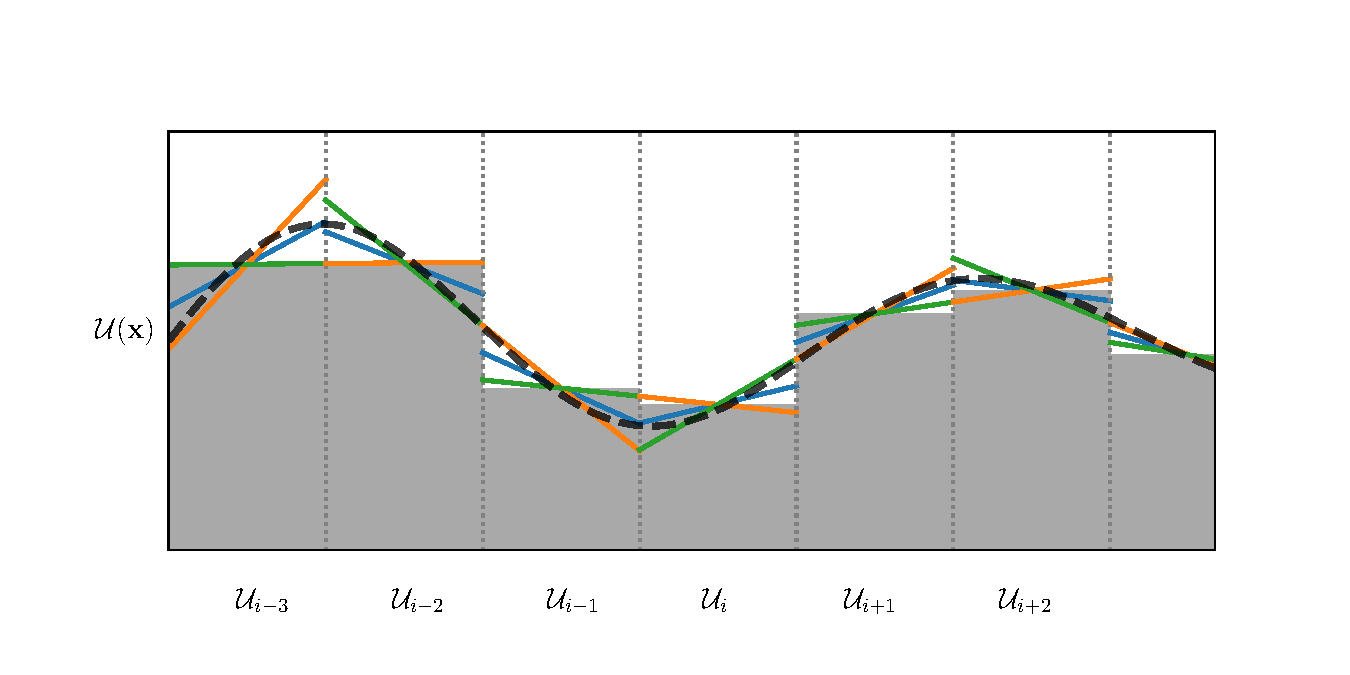
\includegraphics[width=\textwidth]{figures/FV/piecewise_linear.pdf}%
    \caption[Piece-wise linear reconstruction of data]{
Piece-wise linear reconstruction of the data (black dashed line), using different choices for the
slope. The blue lines show the reconstruction using a centered slope, the orange lines are using an
upwind slope, while the green lines use a downwind slope. The gray background represents the the
piece-wise constant reconstruction of the data.
    }
    \label{fig:piecewise-linear}
\end{figure}


A complication that arises as a consequence of moving away from the piece-wise constant
reconstruction of the data is that the solution of the conventional Riemann problem centered at cell
boundaries is not applicable any longer. Instead, the problem at hand is a generalized Riemann
problem with non-constant left and right states $\uc_{i-1}(x)$ and $\uc_{i}(x)$, respectively.
The solution no longer contains uniform regions, and the characteristics are not straight lines any
longer. Unfortunately, the solution for generalized Riemann problems is not available for all
conservation laws, and further approximations need to be made in order to proceed. The
MUSCL-Hancock method prescribes the following approximation: First evolve the boundary extrapolated
values $\uc_L = \uc_i - \frac{\Delta x}{2} s_i$ and $\uc_R = \uc_i + \frac{\Delta x}{2} s_i$ over
half a time step by approximating the state \emph{inside} the cell $i$ as a conventional Riemann
problem with constant states $\uc_L$ and $\uc_R$, i.e. find

\begin{align}
    \overline{\uc}_L &= \uc_L + \frac{\Delta t}{2 \Delta x} (\fc(\uc_L) - \fc(\uc_R))
\label{eq:boundary-extrapolated-L}\\
    \overline{\uc}_R &= \uc_R + \frac{\Delta t}{2 \Delta x} (\fc(\uc_L) - \fc(\uc_R))
\label{eq:boundary-extrapolated-R}
\end{align}

These evolved boundary extrapolated values are then used to approximate the generalized Riemann
problem by as a conventional Riemann problem. Their evolved states serve as an approximation of the average state on the cell boundaries throughout the time step. Consequently the left and right evolved states $\overline{\uc}_{L}$ and $\overline{\uc}_{R}$ are used as the constant states between cell boundaries over the entire time step $\Delta t$. The final update formula is hence given by

\begin{align}
 \uc_i^{n+1} &= \uc_i^n + \frac{\Delta t}{\Delta x} (\fc_{i-\half} - \fc_{i+\half}) \\
 \fc_{i-\half} &= RP(\overline{\uc}_{i-1, R},\ \overline{\uc}_{i,L}) \\
 \fc_{i+\half} &= RP(\overline{\uc}_{i, R},\ \overline{\uc}_{i+1,L})
\end{align}

where $RP(l, r)$ represents the solution of the centered Riemann problem with left state $l$ and
right state $r$ at $x = 0$.









%======================================================================
\subsection{On Monotonicity, Data Compatibility, and Total Variation}
%======================================================================

Figure~\ref{fig:pwlin-gaussian-no-limiter} shows the results of the linear advection using the
MUSCL-Hancock method for the upwind, downwind, and the centered slope on smooth initial conditions.
Compared to the results of the first order method in Figure~\ref{fig:linear-advection-godunov}, it
is obvious that the solution has improved substantially. In this example there is no significant
diffusion any more, which is to be expected since the diffusion term entered as a second order error
in the first order accurate method. This cannot occur in the second order accurate method, as the
second order terms are handled explicitly. However, the situation changes drastically when
discontinuities are involved, as is shown in Figure~\ref{fig:pwlin-step-no-limiter}. The solution
now includes spurious oscillations that evolve and grow over time, which was not the case for the
first order method in Figure~\ref{fig:linear-advection-godunov}. Even worse, because the new
minima and maxima grow with time, they may keep growing to infinity, or other unphysical values.
Clearly they are a serious problem.


\begin{figure}
    \centering
    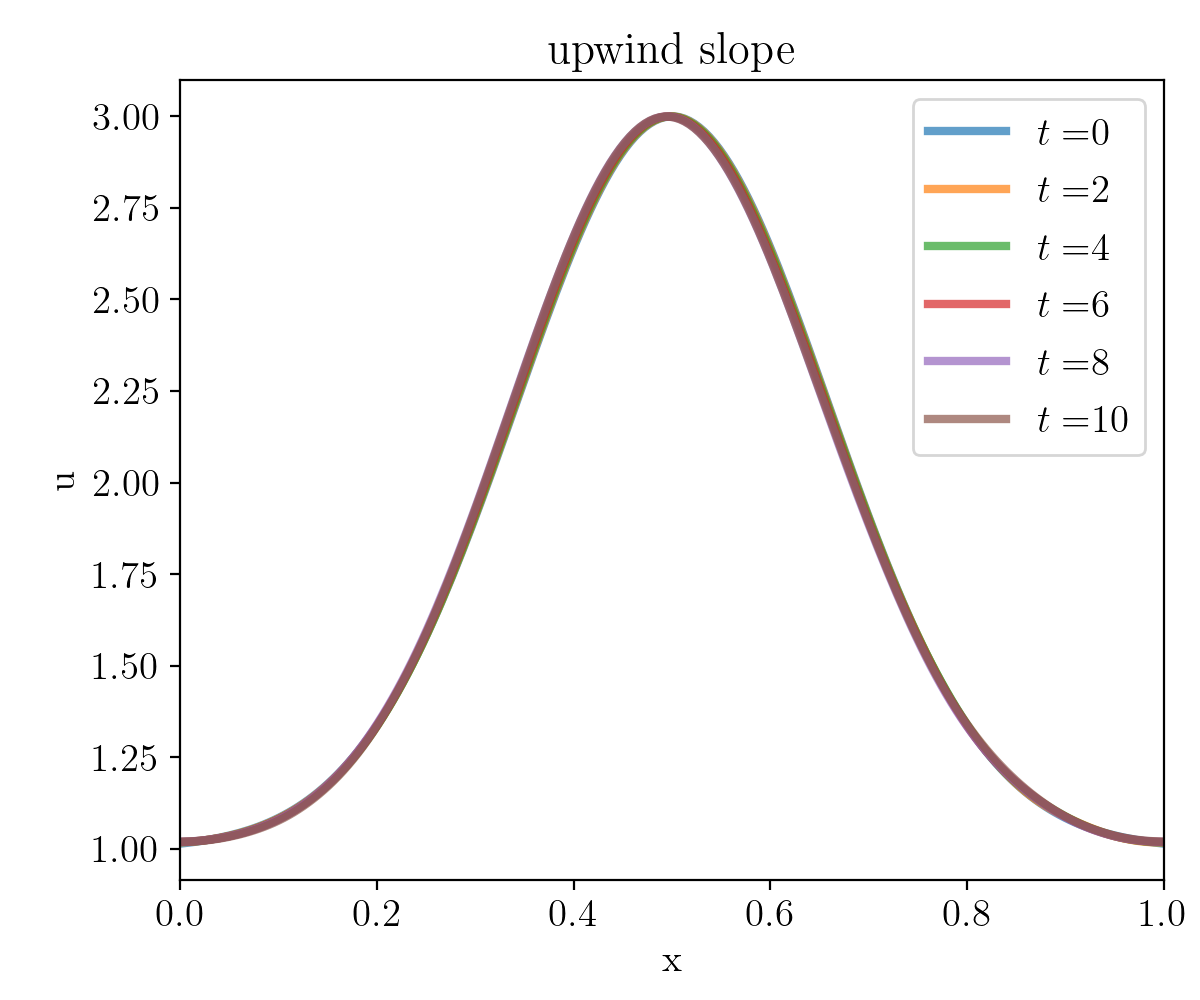
\includegraphics[width=.33\textwidth]{./figures/FV/advection_pwlin/gaussian-upwind.png}%
    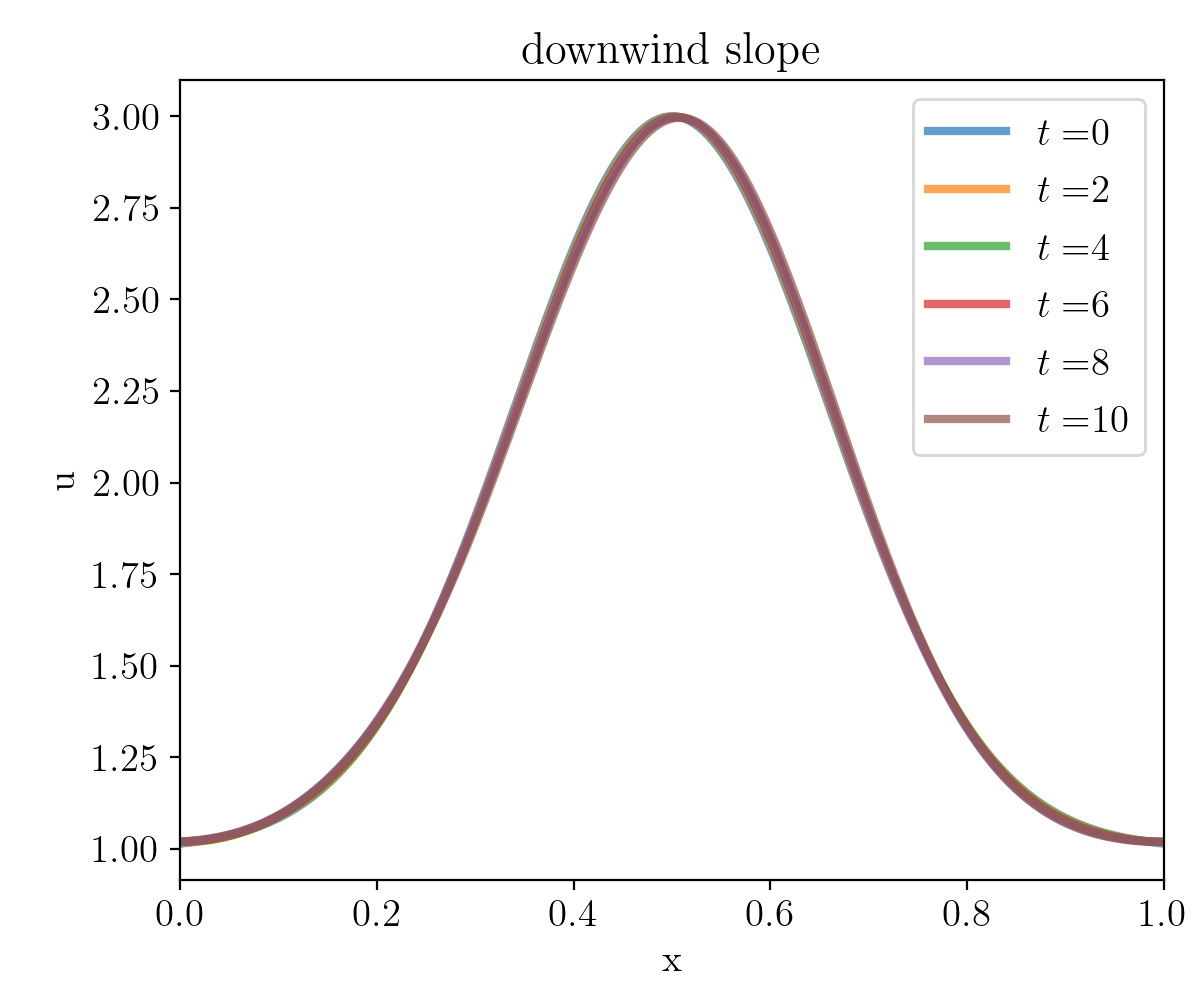
\includegraphics[width=.33\textwidth]{./figures/FV/advection_pwlin/gaussian-downwind.png}%
    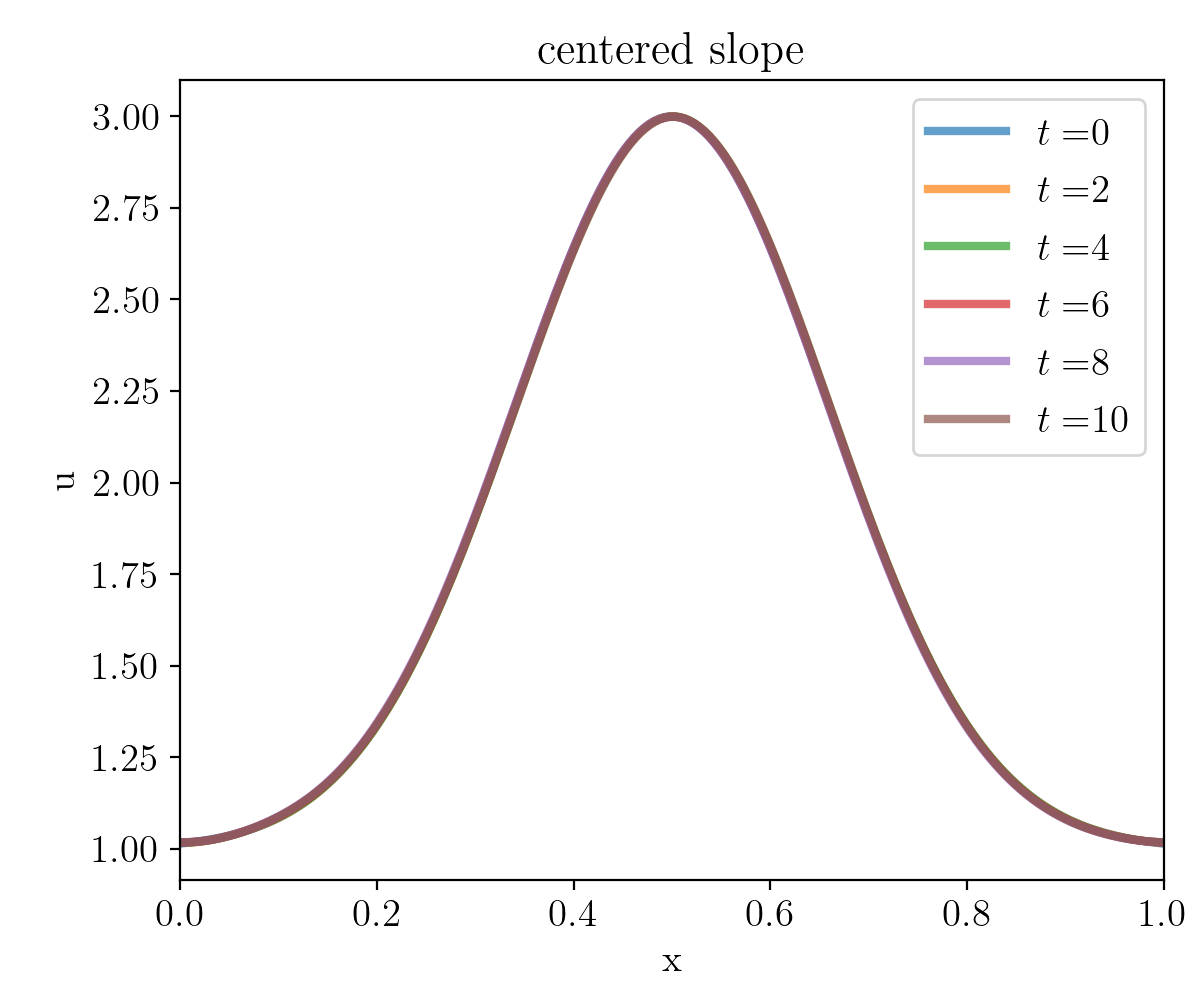
\includegraphics[width=.33\textwidth]{./figures/FV/advection_pwlin/gaussian-centered.png}%
    \caption{
Solution of the linear advection equation using the MUSCL-Hancock method and an upwind (left)
slope, a downwind slope (center), and a centered slope (right) for a smooth Gaussian initial
state with advection coefficient $a = 1$.
    }
    \label{fig:pwlin-gaussian-no-limiter}
\end{figure}

\begin{figure}
    \centering
    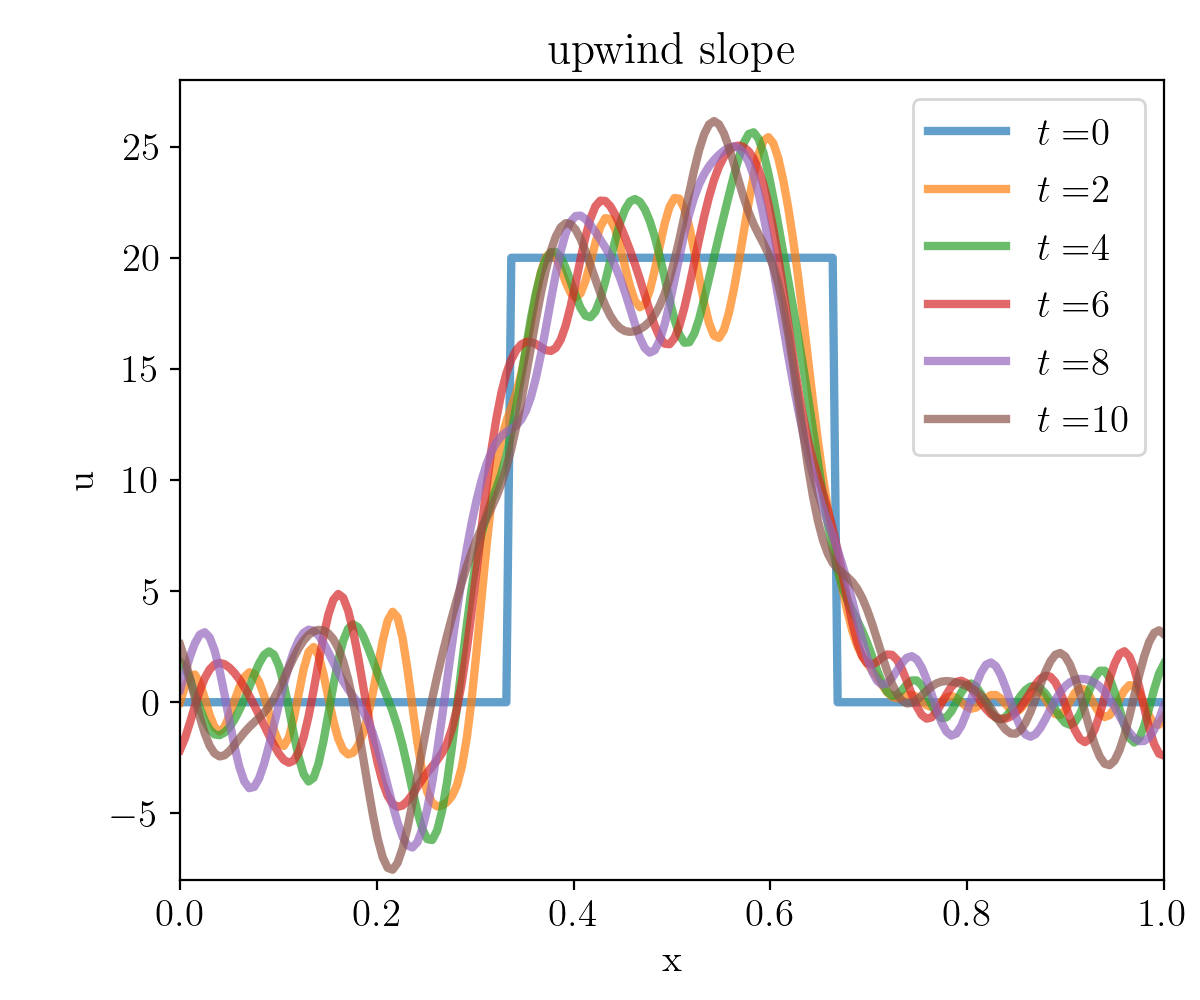
\includegraphics[width=.33\textwidth]{./figures/FV/advection_pwlin/step-upwind.png}%
    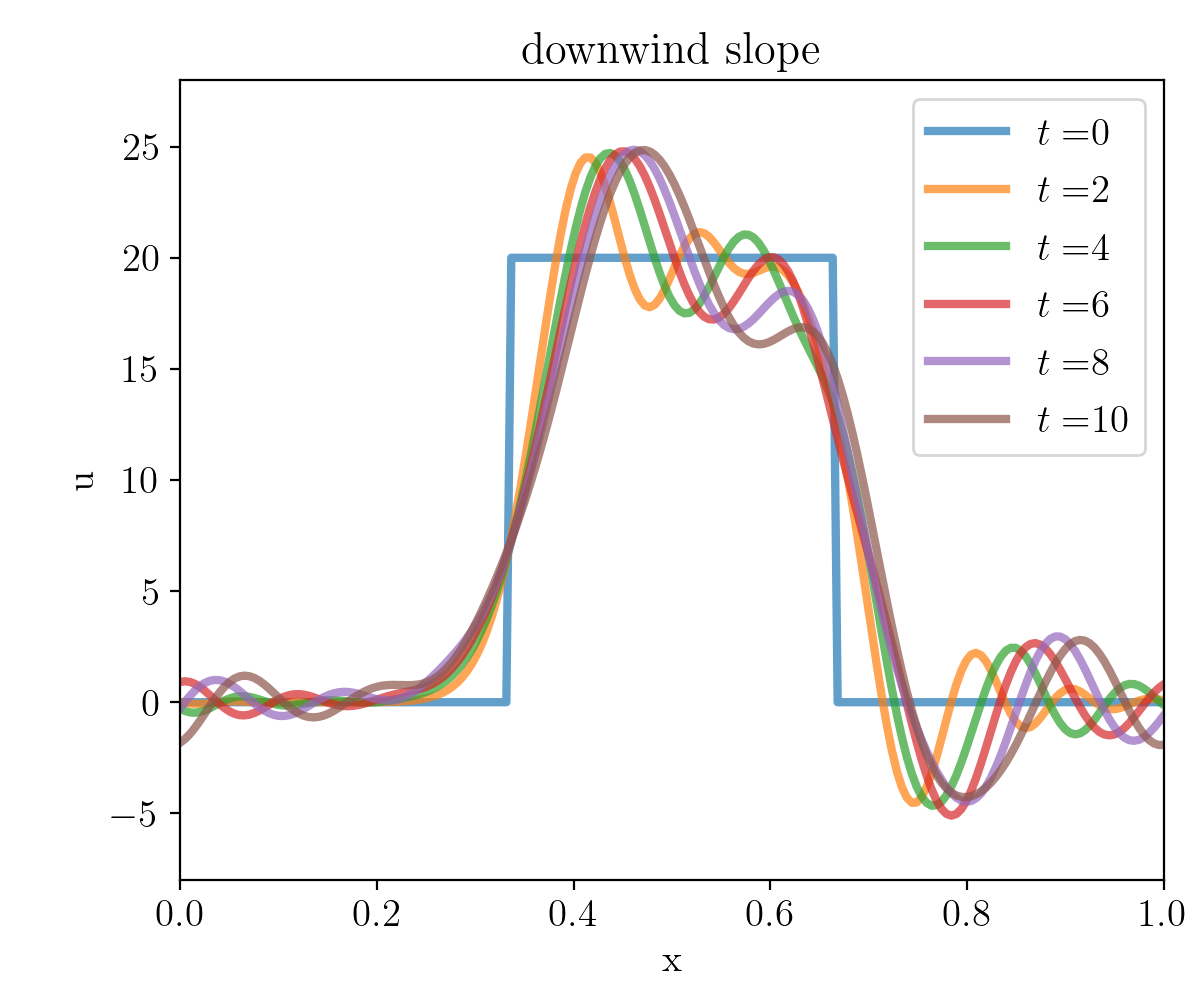
\includegraphics[width=.33\textwidth]{./figures/FV/advection_pwlin/step-downwind.png}%
    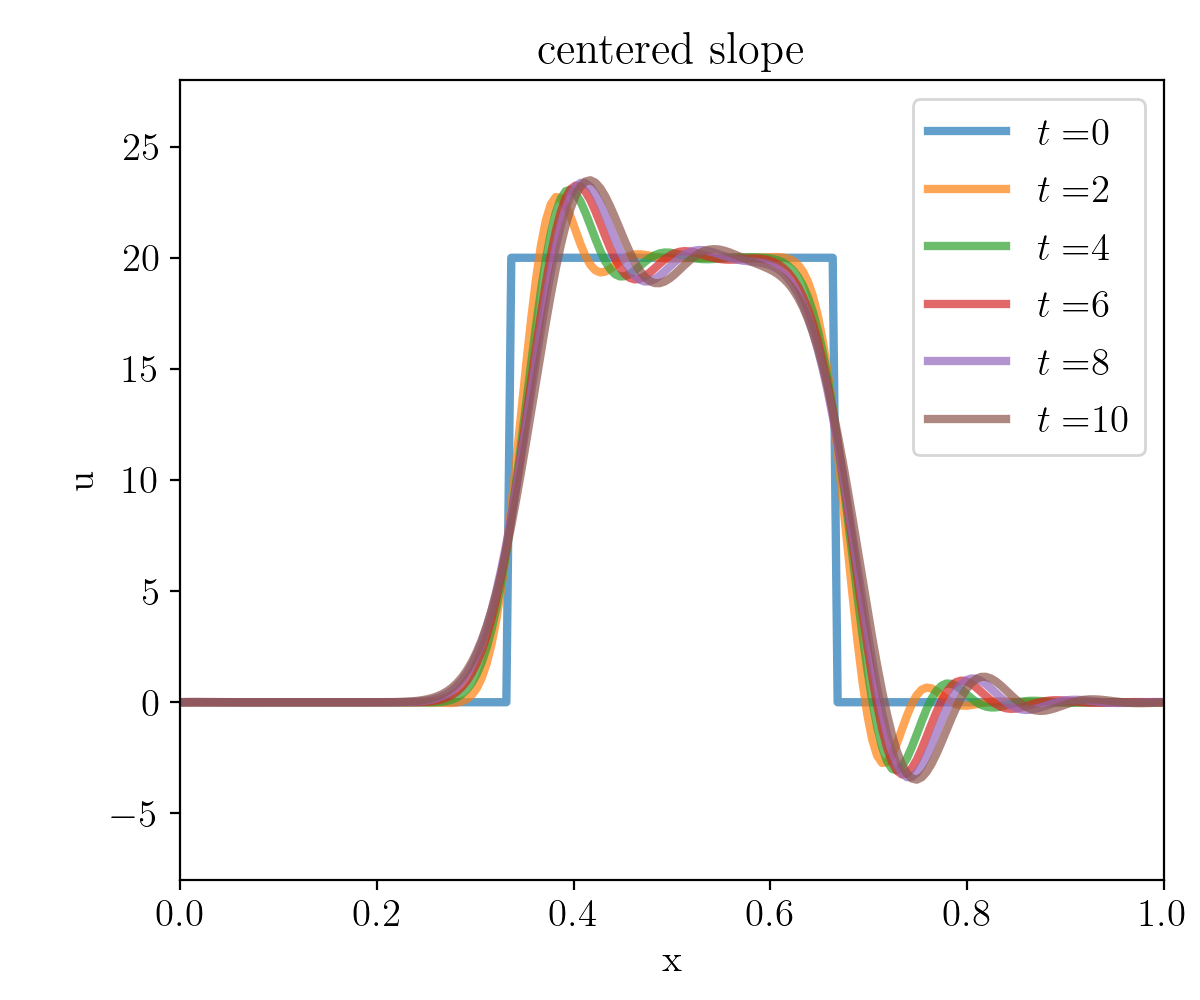
\includegraphics[width=.33\textwidth]{./figures/FV/advection_pwlin/step-centered.png}%
    \caption{
Solution of the linear advection equation using the MUSCL-Hancock method and an upwind (left)
slope, a downwind slope (center), and a centered slope (right) for step function initial
state with advection coefficient $a = 1$.
    }
    \label{fig:pwlin-step-no-limiter}
\end{figure}




These oscillations are a typical phenomenon in higher order schemes. In fact, they are a
consequence of the extension to higher orders. For scalar non-linear conservation laws, this can be
shown by making use of the notion of monotone schemes. A scheme

\begin{align}
    \uc_i^{n+1} = M(\uc_{i-k_l}^n, \hdots, \uc_{i+k_R}^n) = \sum_{k=-k_L+1}^{k_R} b_k \uc_{i+k}^n
\label{eq:monotone-scheme}
\end{align}

with $k_L$, $k_R$ being two non-negative integers is called monotone if

\begin{align}
    \frac{\del M}{\del \uc_j^n} \geq 0 \quad \forall \ j
    \quad \Leftrightarrow \quad
    b_k \geq 0 \quad \forall \ j, k
\end{align}

Since $M$ is a non-decreasing function of all of its arguments, it is equivalent to the following
property:

\begin{align}
    \text{if } v_i^n \geq \uc_i^n \ \forall i, \quad \text{ then } \
    v_i^{n+1} = M(v_i^n) \geq \uc_i^{n+1} = M(\uc_i^n) \ \forall i \label{eq:monotone-2}
\end{align}


If a monotone scheme is applied on some given data set $\{\uc_i^n\}$, then the monotone scheme will
introduce no new minima or maxima, i.e.

\begin{align}
    \max_i \{ \uc_i^{n+1} \} \leq \max_i \{ \uc_i^n \} \label{eq:monotone-max} \\
    \min_i \{ \uc_i^{n+1} \} \geq \min_i \{ \uc_i^n \} \label{eq:monotone-min}
\end{align}

To demonstrate this property, we define $v_i = \max_j \{ u_j^n \} = \CONST \ \forall i$. From the
application of the scalar conservation law

\begin{align}
    \deldt v + \deldx \fc(v) = 0 = \deldt v + \frac{\del \fc}{\del v} \underbrace{\DELDX{v}}_{= 0}
\end{align}

it follows  that $\deldt v = 0$, and $v$ is constant w.r.t. time  as well. Since $v_i = \CONST
\ \forall i$, we can write

\begin{align}
    v_i^{n+1} = M(v_{i - k_L + 1}, \hdots, v_{i+k_R}) = M(v_i) = b_0 v_i
\end{align}

and because it must be constant in time as well, it follows that $b_0 = 1$ and $v_i^{n+1} = v_i^n$.
Using property~\ref{eq:monotone-2} and by definition of $v_i^n = \max_j \{ \uc_j^n \} $,
it follows that

\begin{align}
    v_i^{n+1} =
        v_i^n \geq u_i^{n+1} \quad
        &\Rightarrow \max_j \{ \uc_j^n \} \geq \uc_i^{n+1} \ \forall i,j \\
        &\Rightarrow \max_j \{ \uc_j^n \} \geq \max_j \{ \uc_j^{n+1} \}
\end{align}

The proof for the equivalent relation between minima follows analoguely. For any given time $t^n$
the properties~\ref{eq:monotone-max} and \ref{eq:monotone-min} can be applied recursively back to
$t^0$, which shows that no new minima and maxima will be created by monotone schemes regardless of
the number of time steps taken, and hence no spurious oscillations like in
Figure~\ref{fig:pwlin-step-no-limiter} will be generated. Conversely, it also means that monotone
schemes will clip extrema, as the minima will always increase, while maxima will always decrease.

Unfortunately, there are no monotone, linear schemes for non-linear scalar hyperbolic conservation
laws of second order of accuracy or higher. This fact is known as Godunov's theorem.  It can be
shown using Roe's theorem (see Appendix~\ref{app:roe}), which states that a scheme of the
form~\ref{eq:monotone-scheme} is
$p$-th order accurate if and only if

\begin{align}
    \sum_{k = -k_L}^{k_R} k^q b_k = (-C_{CFL})^q \quad , \quad 0 \leq q \leq p
\end{align}

where $b_k$ are the constant coefficients of the linear scheme, which must be $\geq 0$ for a
monotone scheme. Let

\begin{align}
    S_q \equiv \sum_{k = -k_L}^{k_R} k^q b_k
\end{align}

denote the summation for a single $q$.  Then for a scheme of second order accuracy, we require

\begin{align}
    S_0 = 1, && S_1 = -C_{CFL}, && S_2 = C_{CFL}^2
\end{align}

Explicitly computing $S_2$ reveals

\begin{align}
    S_2
    &= \sum_{k = -k_L}^{k_R} k^2 b_k
    = \sum_{k = -k_L}^{k_R} ([k + C_{CFL}]^2 - 2kC_{CFL} - C_{CFL}^2) b_k \\
    &= \sum_{k = -k_L}^{k_R} [k + C_{CFL}]^2  b_k
    - 2 C_{CFL} \underbrace{\sum_{k = -k_L}^{k_R} k b_k}_{= S_1 = -C_{CFL}}
    - C_{CFL}^2 \underbrace{\sum_{k = -k_L}^{k_R} b_k}_{= S_0 = +1} \\
    &= \sum_{k = -k_L}^{k_R} (k + C_{CFL})^2 b_k + C_{CFL}^2 \label{eq:godunov-theorem-S2}
\end{align}

In order for the scheme to be second order accurate, $S_2$ needs to be equal to $C_{CFL}^2$, which
is only satisfied in two cases. The first case is if $b_k = 0\ \forall k$, which isn't really a
method, since all it does is zero out any initial state. The other case is $C_{CFL} = -k \ \forall
k$. Since there can be only a single Courant number, there can also be only one coefficient index
$k = k_0$, and we need $b_k = 0 \ \forall k \neq k_0$. Furthermore the Courant number must be an
integer, which cannot be the case given the stability requirement $0 < C_{CFL} < 1$. It then
follows that a monotone scheme can't be second order accurate or higher.

If we nevertheless want to make use of schemes of higher order, some adjustments are necessary in
order to avoid spurious oscillations and instabilities around sharp gradients and discontinuities.
However, ideally the adjustments should only take effect close to sharp gradients and
discontinuities, while the second order accurate method should remain unmodified in smooth parts of
the problem. This way we can reap the most benefits from the higher order accuracy. Requiring the
method to behave differently depending on the current state of the problem, i.e. differently in
smooth and discontinuous regions, leads to the core of the approach: The method needs to adapt to
the current state of the problem. This means that a) the coefficients $b_k$ can't be constant any
longer, as they need to adapt according to the situation, and b) we need to find a way to quantify
when and how to modify the method. A way of illustrating the core concept would be to take a closer
look at the results for different choices of the slope in Figure~\ref{fig:pwlin-step-no-limiter}.
In Figure~\ref{fig:pwlin-step-no-limiter}, the advection coefficient is $a = 1$, and the initial
step function travels to the right. The solution using the centered slope for example does quite
well behind the step wave, i.e. at $x \sim 0.3$: there are no spurious oscillations there. But it
introduces a new peak directly in front of the discontinuities at $x \sim 0.4$ and $x \sim 0.7$.
The downwind slope behaves similarly. The upwind slope however deals a bit better with the state in
front of the step wave, i.e. at $x \sim 0.7$, albeit not perfectly. The idea behind an ``adaptive''
method could be to modify the reconstruction of the data by selecting between the different choices
of the slope and pick the ones that promise to give the best results depending on the region. For
example, we could select an upwind slope reconstruction in front of the wave, and a centered slope
behind the step wave. In regions where no linear reconstruction yields acceptable results, for
example around $x \sim 0.4$, we can always fall back on the monotone first order method
(Fig.~\ref{fig:linear-advection-godunov}) which never introduces new extrema.


It remains to establish concrete expressions for the requirements above. One way of ensuring that
a method doesn't develop new extrema is by demanding the algorithm to be ``data compatible''. A
scheme is called compatible with a data set $\{\uc_i^n\}$ if the solution $\{\uc_i^{n+1}\}$ is
bounded by the upwind pair $(\uc_{i-d}^n, \uc_i^n)$, where $d = \text{sign}(C_{CFL}) =
\text{sign}(a)$. This definition can also be written as

\begin{align}
    \min\{\uc_{i-d}^n, \uc_i^n\} \leq \uc_i^{n+1} \leq \max\{\uc_{i-d}^n, \uc_i^n\}
\end{align}

or alternatively

\begin{align}
    0 \leq \frac{\uc_i^{n+1} - \uc_i^n}{\uc_{i-d} - \uc_i^n} \leq 1 \label{eq:data-compatible}
\end{align}

A different way of ensuring that no new extrema form, nor existing extrema grow, is to demand that
the method is total variation diminishing. The total variation $TV$ for a mesh function is defined
as

\begin{align}
    TV(\uc^n) = \sum_i |\uc_{i+1}^n - \uc_i^n |
\end{align}

and a total variation diminishing (TVD) scheme satisfies

\begin{align}
    TV(\uc^{n+1}) \leq TV(\uc^{n}) \label{eq:TVD}
\end{align}

It can be shown that monotone schemes are TVD. An additional neat property of TVD schemes is that
they converge. Equipped with the constraints~\ref{eq:data-compatible} and~\ref{eq:TVD}, we can now
go on to find expressions for modified WAF and MUSCL-Hancock schemes which are both second order
accurate in smooth regions and don't develop spurious oscillations.














%=======================================================
\subsection{TVD Version of the WAF Scheme}\label{chap:WAF-tvd-linear-advection}
%=======================================================


To obtain a TVD version of the WAF scheme, we start off with a more general form of the WAF flux
(eq.~\ref{eq:WAF-flux}) for $a \geq 0$:

\begin{align}
    \fc_{i+\half} = \frac{1}{2} (1 + \phi_{i+\half})(a \uc_i^n) + \frac{1}{2} (1 - \phi_{i+\half})
(a \uc_{i+1}^n)
\end{align}

The goal is to find valid ranges for $\phi$ such that the method is TVD. A first upper and lower
limit for $\phi$ comes from the physical limitations in the extreme case $\phi = \pm 1$, which
corresponds to the characteristic having the maximally allowable velocity, therefore

\begin{align}
    -1 \leq \phi \leq 1
\end{align}


Applying the data compatibility condition~\ref{eq:data-compatible} and after some algebra we arrive
at the inequalities

\begin{align}
    -1 \leq \frac{1}{r_{i+\half}} (1 - \phi_{i+\half}) + \phi_{i-\half} \leq \frac{2 -
|C_{CFL}|}{|C_{CFL}|}
\end{align}

which is valid for both positive and negative $a$, and with the ``flow parameter'' $r_{i+\half}$

\begin{align}
    r_{i+\half} = \begin{cases}
                   \frac{\uc_i^n - \uc_{i-1}^n}{\uc_{i+1}^n - \uc_i^n} & \text{ if } a > 0 \\[6pt]
                   \frac{\uc_{i+2}^n - \uc_{i+1}^n}{\uc_{i+1}^n - \uc_i^n} & \text{ if } a < 0 \\
                  \end{cases}
\end{align}


Additionally, we impose that

\begin{align}
    \phi_{i\pm\half}(r = 1) = |C_{CFL}|
\end{align}

to ensure that the method remains second order accurate in smooth regions where the flow parameter
$r \sim 1$, i.e. where the upwind and downwind slope are nearly identical. As long as
$\phi_{i\pm\half}$ satisfies the above inequalities, the resulting method will be TVD. This means
however that there is any number of possible choices for the ``flux limiter'' $\phi(r)$ that
ensures that the scheme is TVD. To conform with a more general derivation of flux limited methods
by \citet{swebyHighResolutionSchemes1984}, it is practical to write the flux limiter in the form

\begin{align}
    \phi(r) = 1 - (1 - |C_{CFL}|) \psi(r)
\end{align}

to make use of well known expressions for $\psi(r)$ comparable with other methods.
The permissible values for $\psi(r)$ for which it satisfies the inequalities above can be
interpreted as regions on the $r - \psi(r)$ plane. These regions are are shown in
Figure~\ref{fig:flux-limiters-TVD-region} as the gray background, along with some well known limiter
functions:


\begin{flalign}
	\text{Minmod} 								&&\quad \psi(r) &= \mathrm{minmod}(1, r)\\
	\text{Superbee} 							&&\quad \psi(r) &= \max(0, \min(1, 2r), \min(2, r))
\\
	\text{MC (monotonized central-difference)} 	&&\quad \psi(r) &= \max(0, \min ((1+r)/2, 2, 2r))\\
	\text{van Leer}								&&\quad \psi(r) &= \frac{r + |r|}{1 + |r|}
\end{flalign}

where

\begin{align}
	\mathrm{minmod}(a, b) =
		\begin{cases}
			a	& \quad \text{ if } |a| < |b| \text{ and } ab > 0\\
			b	& \quad \text{ if } |a| > |b| \text{ and } ab > 0\\
			0	& \quad \text{ if } ab \leq 0\\
		\end{cases}
\end{align}


\begin{figure}
    \centering
    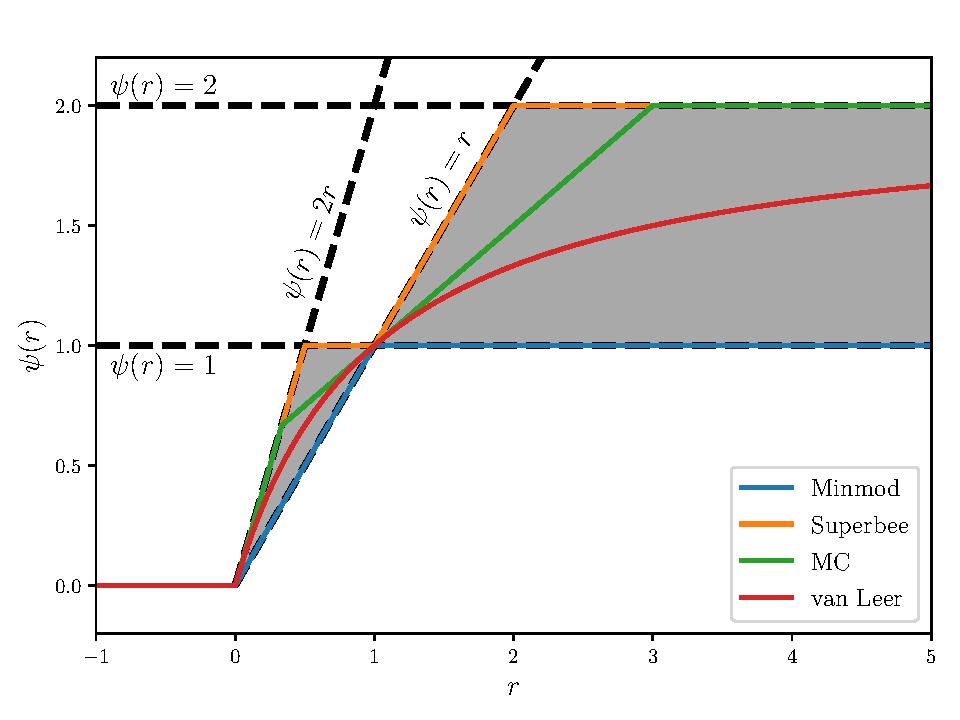
\includegraphics[width=.6\textwidth]{figures/FV/flux_limiters.pdf}%
    \caption[Flux limiters and TVD region]{
Some popular flux limiter functions $\psi(r)$ for the flow parameter $r$. The grey region is the
entire permissible region for the flux limiters within which the inequalities guaranteeing the
method to be TVD are satisfied.
    }
    \label{fig:flux-limiters-TVD-region}
\end{figure}


Figure~\ref{fig:advection-WAF-solution} shows the solution of the linear advection equation using
the WAF method and the various flux limiters described above. None of the solutions that employ a
flux limiter develop spurious oscillations, validating the flux limiting approach. The limiters
display a variety of diffusivity, comparable to the results of the first order method in
Figure~\ref{fig:linear-advection-godunov}. The minmod limiter is the most diffusive one among the
selected limiters, while the superbee limiter displays nearly no diffusivity around discontinuities
at all. However, the superbee limiter tends to clip minima and maxima in smooth regions as well,
and so the top of the Gaussian profile becomes flattened, while the smooth wings get clipped into
discontinuities. This different behavior suggests that there is no general best choice for which
flux limiter to use, and it should be decided based on the underlying problem to be solved.



\begin{figure}
    \centering
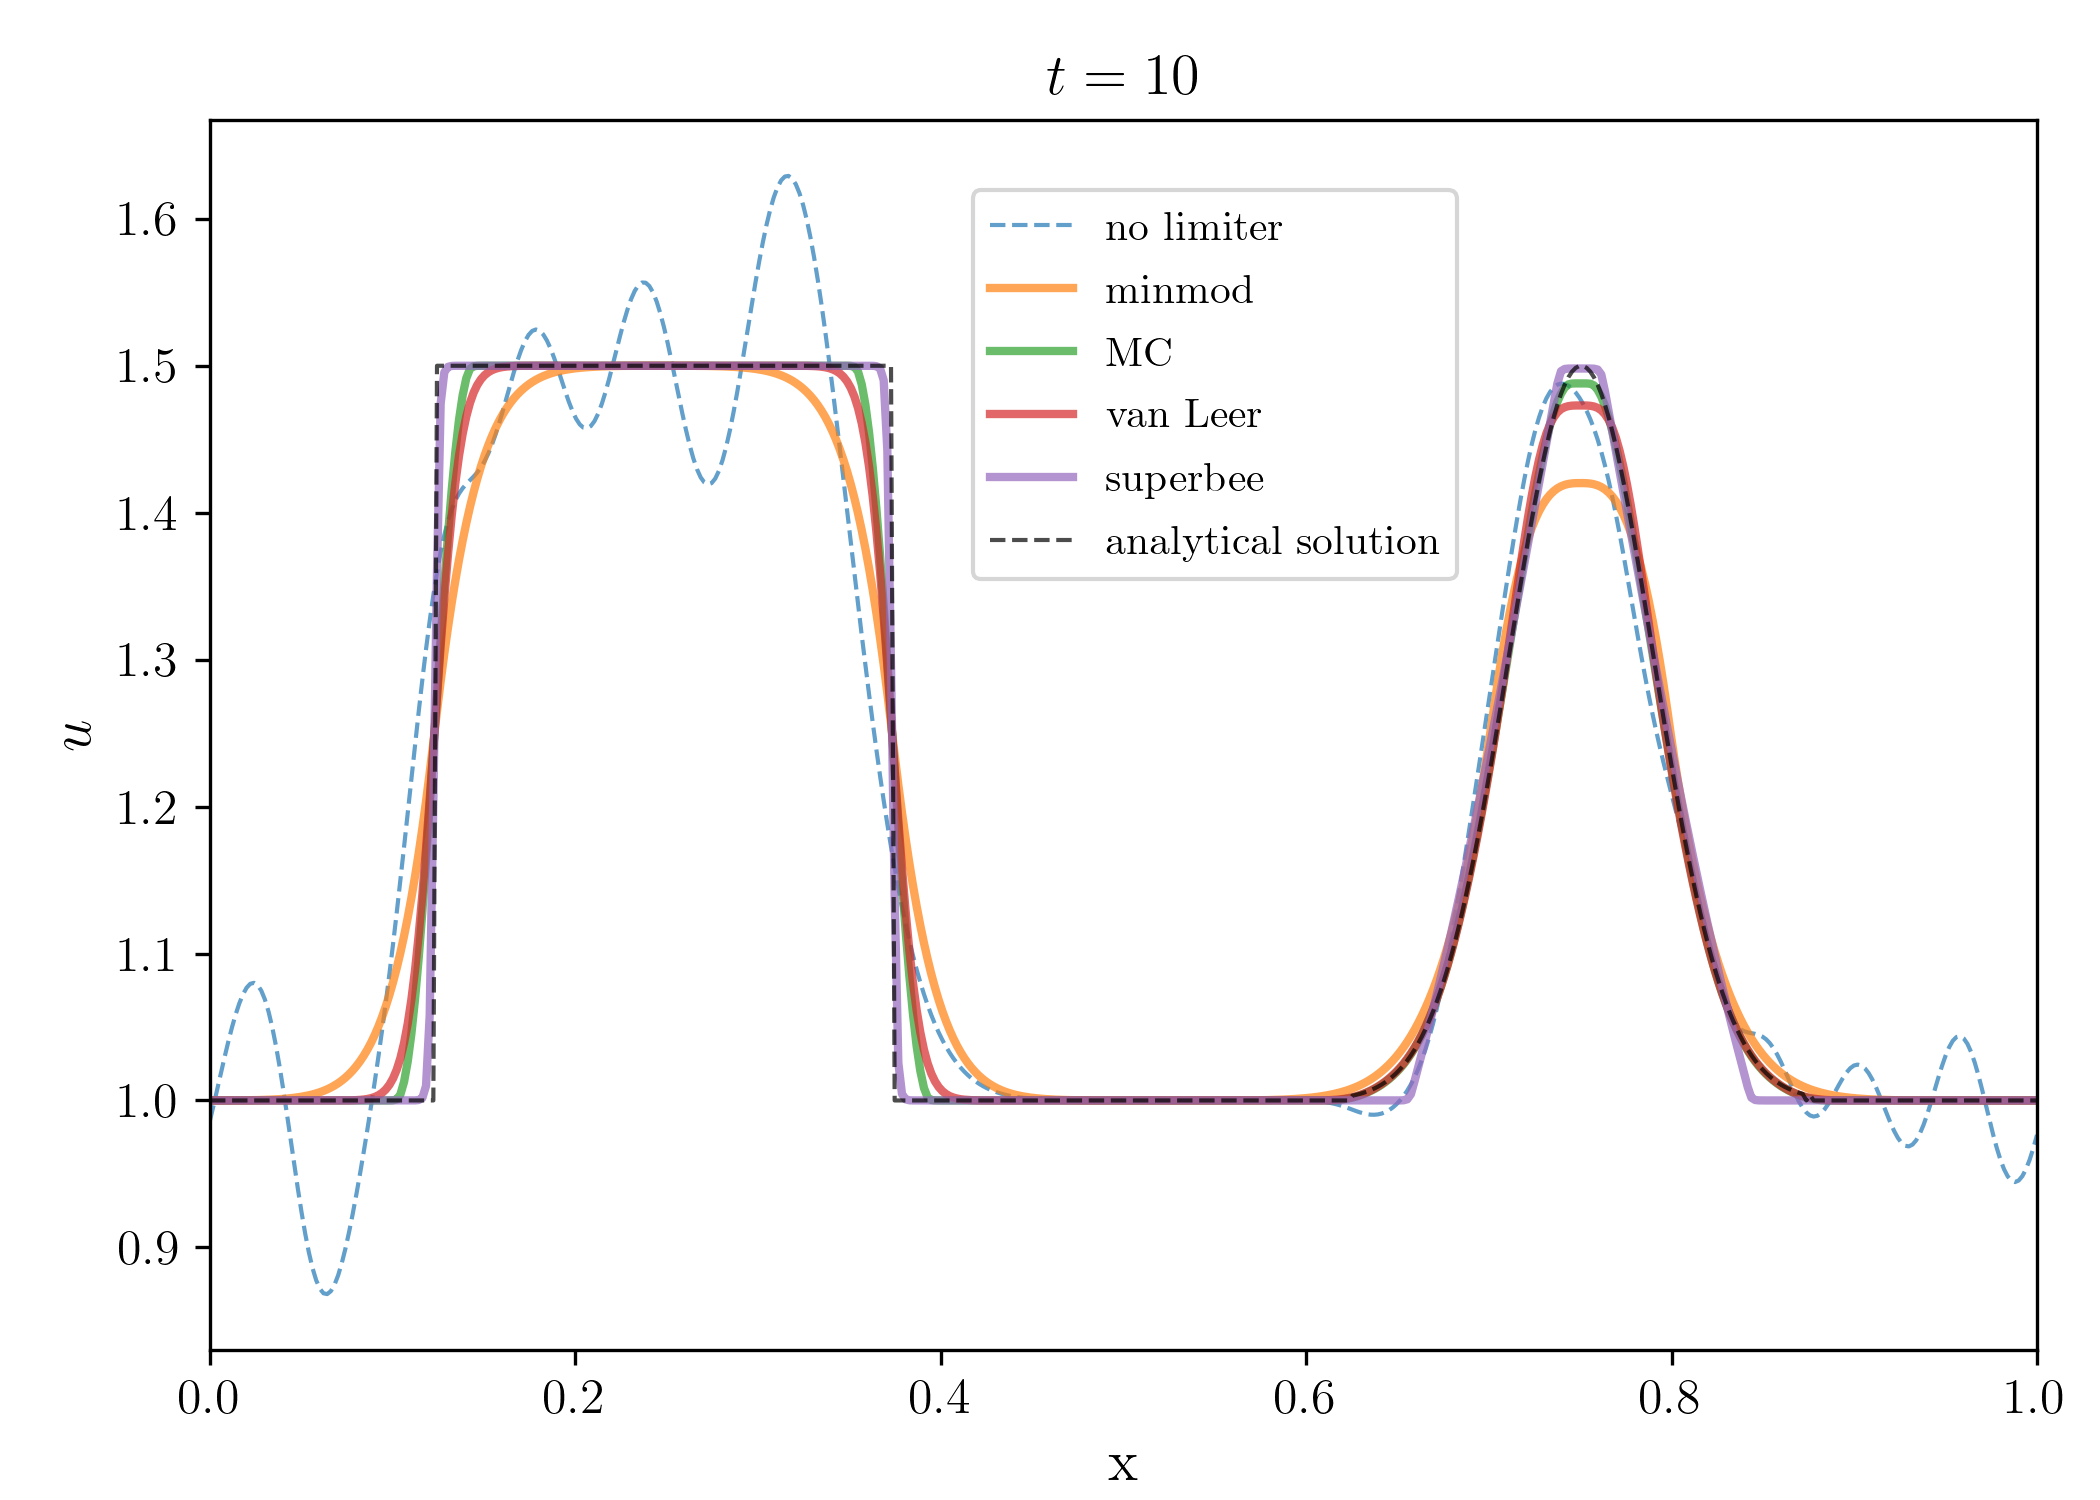
\includegraphics[width=.7\textwidth]{figures/FV/advection_WAF/limiter_comparison-WAF-two-shapes.png}
    \caption[WAF scheme for linear advection with limiters]{
The results for linear advection using the WAF scheme and various flux limiters, compared to the
analytical solution (dashed black line) and the solution without limiters (dashed blue line) for a
step function (left) and a smooth Gaussian (right).
    }
    \label{fig:advection-WAF-solution}
\end{figure}


Finally, let's look at how the order of accuracy of the WAF scheme.
Figure~\ref{fig:advection-WAF-accuracy-dx} shows the average error using various limiters for
smooth Gaussian initial conditions and for a step function for varying $\Delta x$ while keeping
$C_{CFL}$ fixed. Again the errors are measured for both a fixed end time $t_{end} = 2$ of the
simulation, as well as after a fixed number of steps have been completed. For the fixed end time,
the error for the smooth Gaussian indeed decreases with $\propto \Delta x^2$, as the method
promises. However, it quickly converges at $\Delta x \sim 2 \times 10^3$ around the error $10^{-4}$
where it edges on the limits of single precision floating point numbers. After this point, any
further reduction of $\Delta x$ doesn't improve the solution. Since for a fixed $C_{CFL}$ a
decrease of $\Delta x$ means the identical increase in time step size $\Delta t$, decreasing
$\Delta x$ only leads to more time steps being required to reach the specified end time, and
accumulates more errors over more steps. The same applies to the case where the errors are compared
after a fixed number of time steps have been executed: After the point of convergence is reached,
the accuracy doesn't decrease proportional to $\Delta x^2$ any longer, and the order of accuracy is
reduced. While the order of $\Delta x^2$ for the fixed number of time steps is the same as for the
first order method in Figure~\ref{fig:linear-advection-accuracy} for the Gaussian, the order of
$\Delta x^2$ is a clear improvement over the order $\Delta x$ of the first order method. In
particular, note that the absolute value of the error estimate is lower compared to the first order
method by nearly a full order of magnitude even for large $\Delta x$.

In the case of the step function, the improvement in order of accuracy compared to the first order
Godunov method are evident as well. For the experiments run until a fixed end time, the errors
decrease with a slope between $\Delta x^{1/2}$ and $\Delta x$, while in the first order case the
trend was nearly exactly $\Delta x^{1/2}$. For the experiments run over a fixed number of time
steps, the slope of $\Delta x$ is the same in both cases because the presence of the discontinuity
dominates the error term. The fact that discontinuities reduce the order of accuracy of the solution
however persists, and the orders remain lower than in the case of the smooth Gaussian initial
condition.




\begin{figure}
    \centering
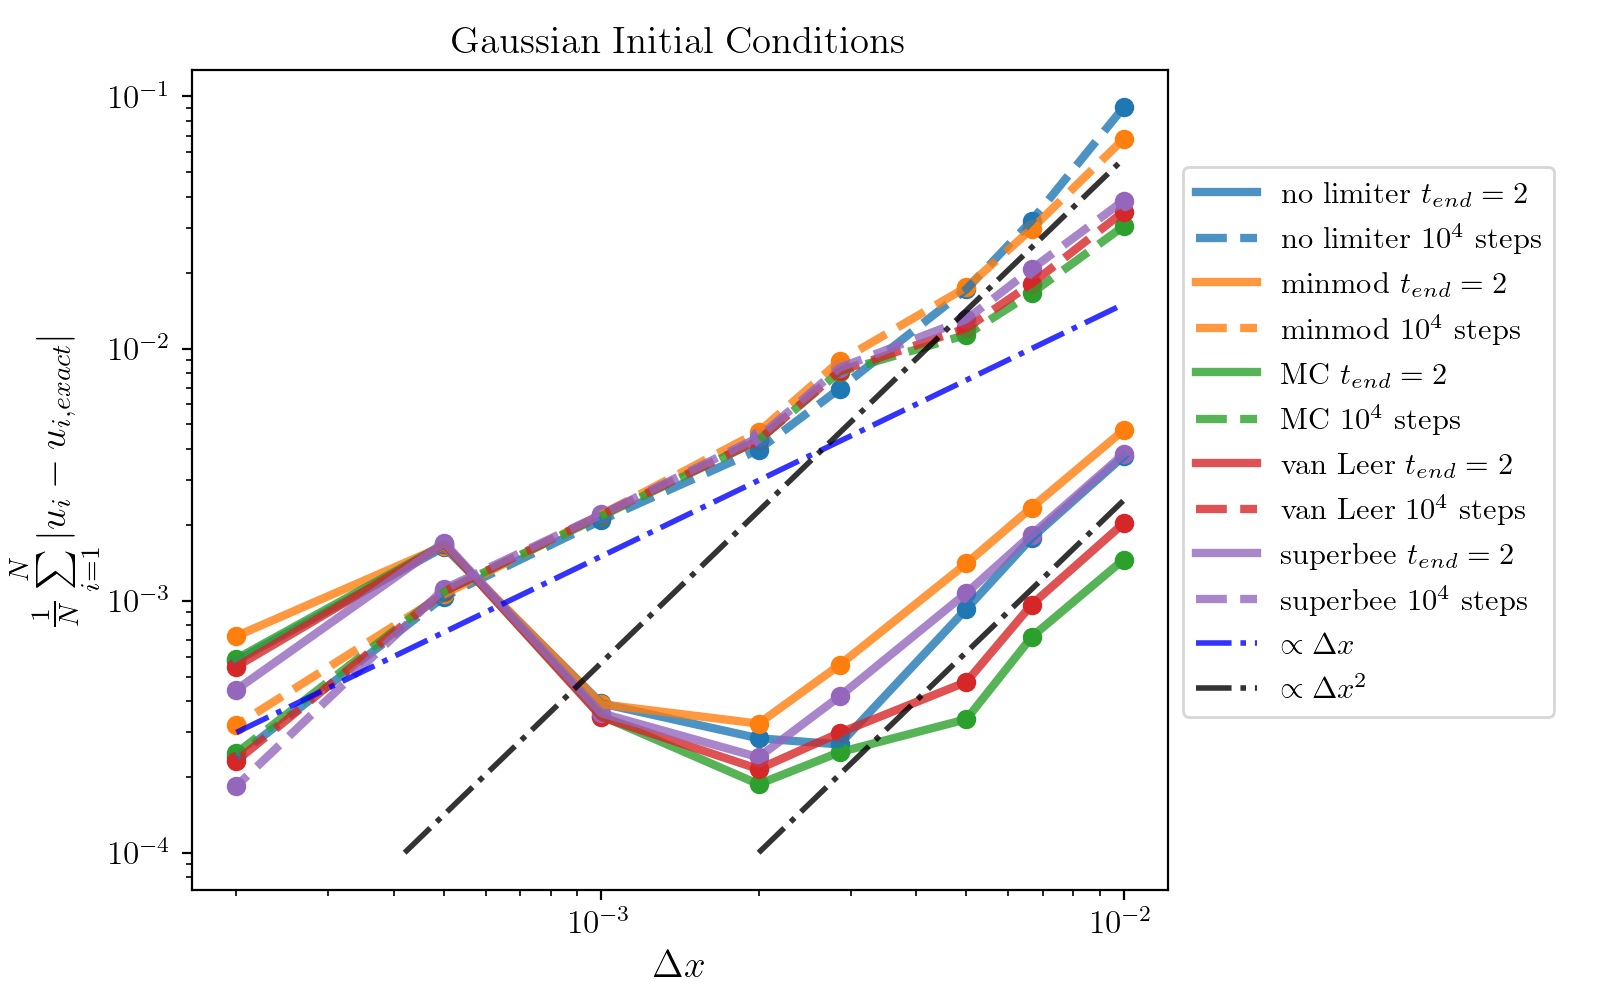
\includegraphics[width=.49\textwidth]{figures/FV/advection_WAF/accuracy_dx-gaussian.png}%
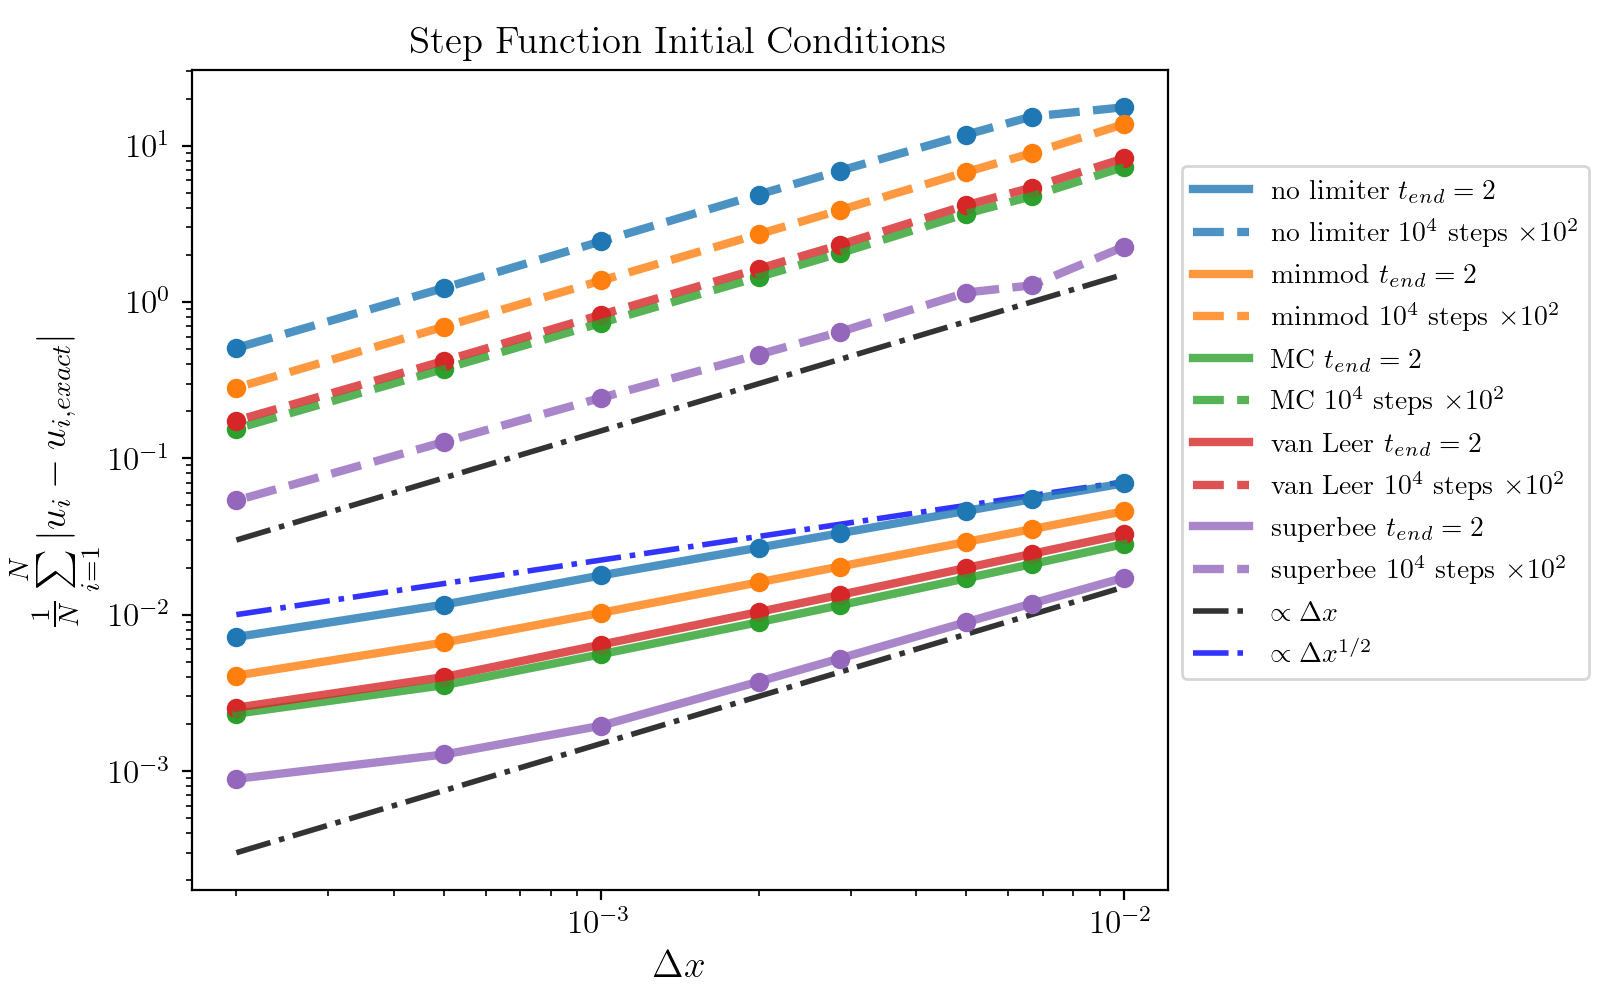
\includegraphics[width=.49\textwidth]{figures/FV/advection_WAF/accuracy_dx-step.png}
    \caption[Order of Accuracy w.r.t. $\Delta x$ for the WAF scheme.]{
The order of accuracy w.r.t $\Delta x$ for the WAF method used for the linear advection equation
with a Gaussian initial condition (left) and a step function (right). The experiments are run for
both a fixed end time $t_{end} = 2$ as well as for fixed number of time steps individually, while
using varying flux limiters. Lines with slopes $1/2$, $1$, and $2$ are over-plotted for comparison.
The results for the step function after a fixed number of steps have been scaled by a factor of
$10^2$ for clarity.
    }
    \label{fig:advection-WAF-accuracy-dx}
\end{figure}











%=======================================================
\subsection{TVD Version of the MUSCL-Hancock Scheme}\label{chap:muscl-hancock-advection-tvd}
%=======================================================


The condition for the MUSCL-Hancock scheme to be TVD can be written as

\begin{align}
    \min_j{\uc_j^n} \leq \uc_i^{n+1} \leq \max_j {\uc_j^n}
\end{align}

with $j \in [i-1, i+1]$.
% More than one neighbouring cell on each side of $\uc_i$ are involved in
% this condition because pairs of cells are required for the computation of the slopes  in the
% piecewise linear reconstruction on each side of $\uc_i$.
This condition can be translated to a condition on the boundary extrapolated values
$\overline{\uc}_{i,L}$ and $\overline{\uc}_{i,R}$
(eqns.~\ref{eq:boundary-extrapolated-L}-\ref{eq:boundary-extrapolated-R}).

\begin{align}
    \min \{ \uc_{i-1}^n, \uc_i^n \} &\leq \overline{\uc}_{i,L} \leq \max \{ \uc_{i-1}^n, \uc_i^n \}
\quad \forall i \\
    \min \{ \uc_{i}^n, \uc_{i+1}^n \} &\leq \overline{\uc}_{i,R} \leq
    \max \{ \uc_{i}^n, \uc_{i+1}^n \} \quad \forall i
\end{align}

To derive more concrete expressions for the inequalities, let's assume that $\uc_{i-1}^n \leq
\uc_i^n$ to start with. Then the inequality reads as

\begin{align}
    \uc_{i-1}^n \leq \overline{\uc}_{i,L} = \uc_i^n - \frac{1}{2}(1 + C_{CFL}) \sigma_i \leq \uc_i^n
\end{align}

where the equality in the middle stems from the definition of $\overline{\uc}_{i,L}$ and $\sigma_i
= s_i \Delta x$. From the left hand side inequality, we find

\begin{align}
    \uc_{i-1}^n - \uc_{i}^n &\equiv -\Delta \uc_{i-\half} \leq - \frac{1}{2}(1 + C_{CFL}) \sigma_i \\
    \sigma_i &\leq \frac{2}{1 + C_{CFL}} \Delta \uc_{i-\half}
\end{align}

where we defined $\Delta \uc_{i-\half} = \uc_{i}^n - \uc_{i-1}^n$. From the second inequality, we
obtain

\begin{align}
    \uc_{i}^n - \frac{1}{2}(1 + C_{CFL}) \sigma_i &\leq \uc_i^n\\
    - \frac{1}{2}(1 + C_{CFL}) \sigma_i &\leq \uc_i^n - \uc_i^n = 0\\
    \sigma_i &\geq 0
\end{align}

Finally giving us

\begin{align}
 0 \leq \sigma_i \leq \frac{2}{1 + C_{CFL}} \Delta \uc_{i-\half} &&
 \text{ if } \Delta \uc_{i-\half} \geq 0
\end{align}

The same exercise can be repeated by assuming $\uc_i^n \leq \uc_{i-1}^n$, i.e. $\Delta
\uc_{i-\half} \leq 0$ to obtain


\begin{align}
 0 \geq \sigma_i \geq \frac{2}{1 + C_{CFL}} \Delta \uc_{i-\half} &&
 \text{ if } \Delta \uc_{i-\half} \leq 0
\end{align}

and by using the second inequality for $\overline{\uc}_{i,R}$ and again considering both cases
$\Delta \uc_{i+\half} \geq 0$ and $\Delta \uc_{i+\half} \leq 0$, two more conditions are found:


\begin{align}
 0 \leq \sigma_i &\leq \frac{2}{1 - C_{CFL}} \Delta \uc_{i+\half} &&
 \text{ if } \Delta \uc_{i+\half} \geq 0 \\
 0 \geq \sigma_i &\geq \frac{2}{1 - C_{CFL}} \Delta \uc_{i+\half} &&
 \text{ if } \Delta \uc_{i+\half} \leq 0
\end{align}


An immediate first result is that in case $\Delta \uc_{i-\half}$ and $\Delta \uc_{i+\half}$ have
opposite signs, the conditions reduce to $0 \geq s_i \leq 0$, and the only possible solution is
$s_i = 0$. If they have the same sign however, the above inequalities give us upper limits, which
can be combined into a single upper boundary:

\begin{align}
    \sigma_i \leq \min \left\{\frac{2}{1 - C_{CFL}} | \Delta \uc_{i+\half}|, \frac{2}{1 + C_{CFL}}
|\Delta \uc_{i-\half}| \right\}
\end{align}


To find methods that satisfy these conditions, the estimated slopes $\sigma_i$ of the MUSCL-Hancock
method are modified to slope limited slopes $\overline{\sigma}_i$ that contain a slope limiter
$\xi(r)$.
For a general slope $\sigma_i$ of the form

\begin{align}
    \sigma_i =
    \frac{1}{2} (1 + \omega) \Delta \uc_{i-\half} +
    \frac{1}{2} (1 - \omega) \Delta \uc_{i+\half}
\end{align}

the limited slope is given by

\begin{align}
    \overline{\sigma}_i  = \xi(r) \sigma_i
\end{align}

where $r$ is the flow parameter

\begin{align}
    r = \frac{\Delta \uc_{i-\half}}{\Delta \uc_{i+\half}}
\end{align}

and the TVD conditions can hence be written in terms of $\xi(r)$ as

\begin{align}
\xi(r) &= \begin{cases}
          0 & \text{ if }  r \leq 0 \\
          \leq \min \{ \xi_L, \xi_R \} & \text{ if } r > 0
         \end{cases} \\
\xi_L(r) &= \frac{\frac{4r}{(1 + C_{CFL})}}{1 - \omega + (1 + \omega) r} \\
\xi_R(r) &= \frac{\frac{4}{(1 - C_{CFL})}}{1 - \omega + (1 + \omega) r}
\end{align}

Once again any number of functions $\xi(r)$ that satisfy the above conditions are imaginable, and
hence many possible choices for slope limiters exist. Some popular limiters are:

\begin{flalign}
	\text{Minmod} 								&&\quad \xi(r) &=
					\begin{cases}
						0, & r \leq 0\\
						r, & 0 \leq r \leq 1\\
						\min\{1, \xi_R(r)\}, & r \geq 1\\
					\end{cases}
			\\
	\text{Superbee} 							&&\quad \xi(r) &=
						\begin{cases}
							0, & r \leq 0\\
							2r, & 0 \leq r \leq \frac{1}{2}\\
							1, & \frac{1}{2} \leq r \leq 1 \\
							\min\{r, \xi_R(r), 2\}, & r \geq 1\\
						\end{cases}
				\\
	\text{van Leer}								&&\quad \xi(r) &=
						\begin{cases}
							0, & r \leq 0\\
							\min\{\frac{2r}{1+r},  \xi_R(r)\}, & r \geq 0\\
						\end{cases}
\end{flalign}


Note that these slope limiters are not equivalent to the flux limiters bearing the same name, but
are analogous. For example, the Superbee limiters both follow the upper edge for of their
respective TVD regions, but are not identical expressions.



















%=======================================================
\section{Higher Order Schemes For The Euler Equations}
%=======================================================




%=======================================================
\subsection{The WAF Scheme}
%=======================================================

The WAF scheme for the Euler equations also estimates the fluxes at the midpoint in time by using
an integral average

\begin{align}
\F_{i+\half}^{WAF} = \frac{1}{\Delta x} \int\limits_{-\half \Delta x}^{\half \Delta x}
    \F(\U_{i+\half}) \de x \label{eq:WAF-flux-euler}
\end{align}

where $\U_{i+\half}$ is the solution of the Riemann problem with piece-wise constant data $\U_i^n$
and $\U_{i+1}^n$ centered at the position $x = x_{i+\half}$. Instead of a single wave emanating as
the solution of the Riemann problem for the linear advection equation, for the Euler equations we
obtain three waves, which separate the $x-t$ plane into 4 regions $\U_L$, $\U_L^*$, $\U_R^*$, and
$\U_R$. Naming the points $(x_k,\Delta t/2)$ plane where the characteristics of the three waves $k$
are situated at the time $\Delta t / 2$ as $A_k$, (see Figure~\ref{fig:hydro-WAF-setup}), and
choosing the indices $k$ such that the wave velocities $S_1 < S_2 < S_3$, then the distances
between these points are given by

\begin{align}
    \overline{A_0 A_1} &= \frac{\Delta x}{2} (1 + C_1) \\
    \overline{A_1 A_2} &= (C_2 - C_1) \frac{\Delta x}{2} \\
    \overline{A_2 A_3} &= (C_3 - C_2) \frac{\Delta x}{2} \\
    \overline{A_3 A_4} &= (1 - C_3) \frac{\Delta x}{2} \\
    C_k &\equiv \frac{S_k \Delta t}{\Delta x}
\end{align}


The integral~\ref{eq:WAF-flux-euler} can then be performed separately between each two adjacent
points $A_k$, $A_{k+1}$. Rarefaction waves require some special attention, since they contain a
fan between the head and the tail waves, which is composed of a smooth transition, not a constant
state. While technically an analytical solution to the integral over the rarefaction fan can be
found, experience shows that an approximation is sufficiently accurate. The approximation is to
simply ``lump'' the fan together with the closest adjacent constant state, where ``closest'' is
with regards to the distance from the center, i.e. the $t$-axis. This special treatment for
rarefactions is not necessary for HLL type Riemann solvers, whose solution is the flux itself, not
the individual states.



\begin{figure}
    \centering
    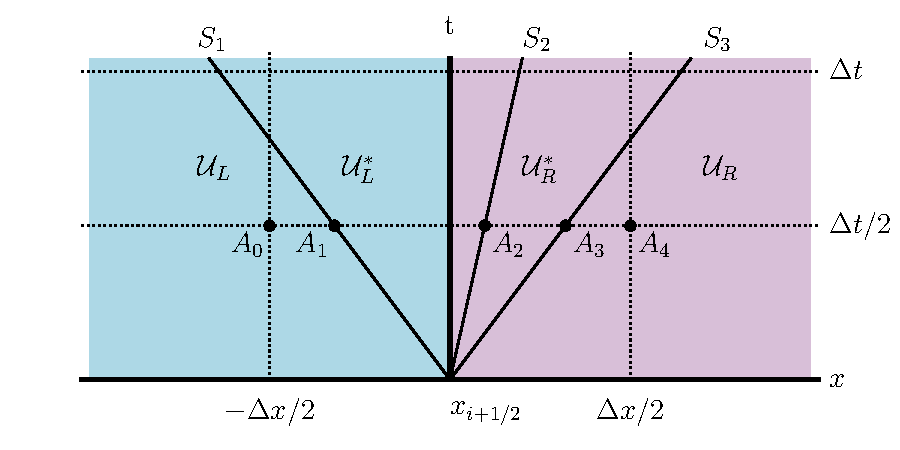
\includegraphics[width=.8\linewidth]{figures/FV/WAF-hydro.pdf}
    \caption[Setup for the WAF method for Euler equations]{
        Sketch for the set-up for the WAF method for Euler equations.
    }%
    \label{fig:hydro-WAF-setup}
\end{figure}


The WAF flux then takes the form

\begin{align}
    \F_{i+\half}^{WAF} &= \sum_{k=1}^4 \frac{1}{2} (C_k - C_{k-1}) \F^{(k)} \\
    &= \frac{1}{2} \left( \F_i + \F_{i+1} \right) -
    \frac{1}{2} \sum_{k=1}^3 C_k (\F^{(k+1)} - \F^{(k)})
\end{align}


A TVD modification of the WAF flux is

\begin{align}
    \F_{i+\half}^{WAF} &=
        \frac{1}{2} \left( \F_i + \F_{i+1} \right) -
        \frac{1}{2} \sum_{k=1}^3 \mathrm{sign}(C_k) \phi_{i+\half}^{(k)} (\F^{(k+1)} - \F^{(k)})
\end{align}

where

\begin{align}
    \phi_{i+\half} ^{(k)} &= \phi_{i+\half}(r^{(k)}) \\
    r^{(k)} &= \begin{cases}
                \frac{\Delta q_{i-\half}^{(k)}}{\Delta q_{i+\half}^{(k)}} & \text{ if } C_k > 0 \\
                \frac{\Delta q_{i+3/2}^{(k)}}{\Delta q_{i+\half}^{(k)}} & \text{ if } C_k < 0
               \end{cases}
\end{align}

$q$ is a single quantity which is known to change across each wave $k$, for example density or
internal energy. For the limiters $\phi_{i+\half}$, the same expressions as in
Section~\ref{chap:WAF-tvd-linear-advection} may be used.
This extension for to a TVD form of the WAF method for Euler equations is somewhat empirical, and
there is no rigorous proof that it will actually remain TVD in every conceivable case, but is found
to work well in practice. The reason is that in order to demonstrate the TVD properties of the
scheme for the linear advection, we made heavy use of the analytical solution of the linear
advection equation. Doing the same for Euler equations while covering all possible outcomes for any
initial conditions for the Riemann problems that need to be solved is a daunting task, and so we
need to rely on the findings in the simpler case of the linear advection.












%=======================================================
\subsection{The MUSCL-Hancock Scheme}
%=======================================================

The MUSCL-Hancock Scheme for Euler equations follows the same steps as the one for linear
advection, with the difference that instead of a single scalar quantity $\uc$, now a state vector
$\U$ is being represented through piece-wise linear reconstructions of the field, i.e.

\begin{align}
    \U_i = \U_i(x) = \U_i^n + \frac{x - x_i}{\Delta x} S_i \quad, \quad x \in [0, \Delta x]
\end{align}

where $S_i$ is now a vector containing a slope of each component of $\U$. The values of $\U_i$ at
the boundaries $x_{i \pm \half}$ are analoguely given by

\begin{align}
    \U_L = \U_i^n - \frac{1}{2} S_i && \U_R = \U_i^n + \frac{1}{2} S_i
\end{align}

Again the boundary extrapolated values are evolved for half a time step using

\begin{align}
    \overline{U}_L &= \U_{i,L} + \frac{1}{2}\frac{\Delta t}{\Delta x} [\F(\U_{i,L})- \F(\U_{i,R})]\\
    \overline{U}_R &= \U_{i,R} + \frac{1}{2}\frac{\Delta t}{\Delta x} [\F(\U_{i,L})- \F(\U_{i,R})]\\
\end{align}

These evolved boundary extrapolated values are then used to approximate the generalized Riemann
problem by solving a conventional Riemann problem with constant left and right evolved states
$\U_{L}$ and $\U_{R}$ between cell boundaries over the entire time step $\Delta t$. The final
update formula is hence given by

\begin{align}
 \U_i^{n+1} &= \U_i^n + \frac{\Delta t}{\Delta x} (\F_{i-\half} - \F_{i+\half}) \\
 \F_{i-\half} &= RP(\overline{\U}_{i-1, R},\ \overline{\U}_{i,L}) \\
 \F_{i+\half} &= RP(\overline{\U}_{i, R},\ \overline{\U}_{i+1,L})
\end{align}

where $RP(l, r)$ represents the solution of the centered Riemann problem with left state $l$ and
right state $r$ at $x = 0$. The TVD version of the method is obtained by limiting the slopes $S_i$
for each component individually in the same manner it is done for the linear advection equation in
Section~\ref{chap:muscl-hancock-advection-tvd}: The slope $S_i$ is replaced by the slope limited
version $\overline{S}_i$

\begin{align}
    S_i^k = \xi_i^k S_i^k
\end{align}

for each component $k$ of the state vector $\U$. The same slope limiters as listed in
Section~\ref{chap:muscl-hancock-advection-tvd} may be employed.

To showcase the improvements that follow using a second order method with limiters
for the Euler equations, Figures~\ref{fig:MUSCL-sod-test},~\ref{fig:MUSCL-left-blast-wave},
and~\ref{fig:MUSCL-two-shocks} show the solution of various Riemann problems using the MUSCL-Hancock
method and Godunov's method. For clarity, only the results using the Van Leer slope limiter are
shown, along with the solution when using no limiter at all. In all cases, the better treatment of
discontinuities compared to Godunov's first order method are obvious, and the spurious oscillations
visible in the solution without a slope limiter disappear as well.

The difference in results between a first and second order scheme can perhaps be better illustrated
using a two-dimensional example where mixing of several fluid phases occurs. A fitting example is
the Kelvin-Helmholtz instability, which arises when two fluid phases shear past each other on a
slightly perturbed interface. The initial conditions are taken from
\citet{mcnallyWellposedKelvinHelmholtzInstability2012} and prescribe the following density inside a
periodic two dimensional box of size unity in each dimension:

\begin{align}
\rho(x,y) = \begin{cases}
            \rho_1 - \overline{\rho} \exp \left( \frac{y - 1/4}{L} \right) &
                \text{ if } 0 \leq y < 1/4 \\
            \rho_2 + \overline{\rho} \exp \left( \frac{1/4 - y}{L} \right) &
                \text{ if } 1/4  \leq y < 1/2 \\
            \rho_2 + \overline{\rho} \exp \left( \frac{y - 3/4}{L} \right) &
                \text{ if } 1/2  \leq y < 3/4 \\
            \rho_1 - \overline{\rho} \exp \left( \frac{3/4 - y}{L} \right) &
                \text{ if } 3/4 \leq y \leq 1
            \end{cases}
\end{align}

where $\overline{\rho} = (\rho_1 - \rho_2) / 2$, $\rho_1 = 1$, $\rho_2 = 2$, and $L = 0.025$. To
obtain a shearing motion of the phases, the velocity of the fluid in $x$ direction is set up as

\begin{align}
v_x(x,y) = \begin{cases}
            v_1 - \overline{v} \exp \left( \frac{y - 1/4}{L} \right) &
                \text{ if } 0 \leq y < 1/4 \\
            v_2 + \overline{v} \exp \left( \frac{1/4 - y}{L} \right) &
                \text{ if } 1/4  \leq y < 1/2 \\
            v_2 + \overline{v} \exp \left( \frac{y - 3/4}{L} \right) &
                \text{ if } 1/2  \leq y < 3/4 \\
            v_1 - \overline{v} \exp \left( \frac{3/4 - y}{L} \right) &
                \text{ if } 3/4 \leq y \leq 1
            \end{cases}
\end{align}

where again $\overline{v} = (v_1 - v_2) / 2$ and $v_1 = 0.5$, $v_2 = -0.5$. Finally, the small
perturbation in the shear is added by giving a small velocity in $y$ direction:

\begin{align}
    v_y(x,y) = 0.01 \sin(4\pi x)
\end{align}

The initial pressure is set everywhere to $p = 2.5$. The results using these initial conditions
with the \meshhydro code on a grid of size $256 \times 256$ for Godunov's method and the
MUSCL-Hancock scheme with the Van Leer limiter are shown in
Figures~\ref{fig:kelvin-helmholtz-1}~and~\ref{fig:kelvin-helmholtz-2}. As time evolves, the initial
perturbations grow, and peaks arise at the interface of the two fluid phases, which penetrate into
the other phase. Eventually these peaks begin to curl up, giving rise to the typical
Kelvin-Helmholtz whirls, as can be seen in the bottom row of Figure~\ref{fig:kelvin-helmholtz-1}.
Both Godunov's scheme and the MUSCL-Hancock scheme are able to reproduce this behavior, although
the contact discontinuities in the results of the MUSCL-Hancock scheme are clearly sharper. However
at later times, shown in Figure~\ref{fig:kelvin-helmholtz-2}, differences become much more obvious.
The MUSCL-Hancock method is able to resolve much more fine structure, while Godunov's method cannot
due to its diffusivity. By the end of the simulation, Godunov's method predicts a nearly fully
mixed interface region, while the MUSCL-Hancock scheme still finds some fine structure along the
interface and inside the whirls.





\begin{figure}
   \centering
   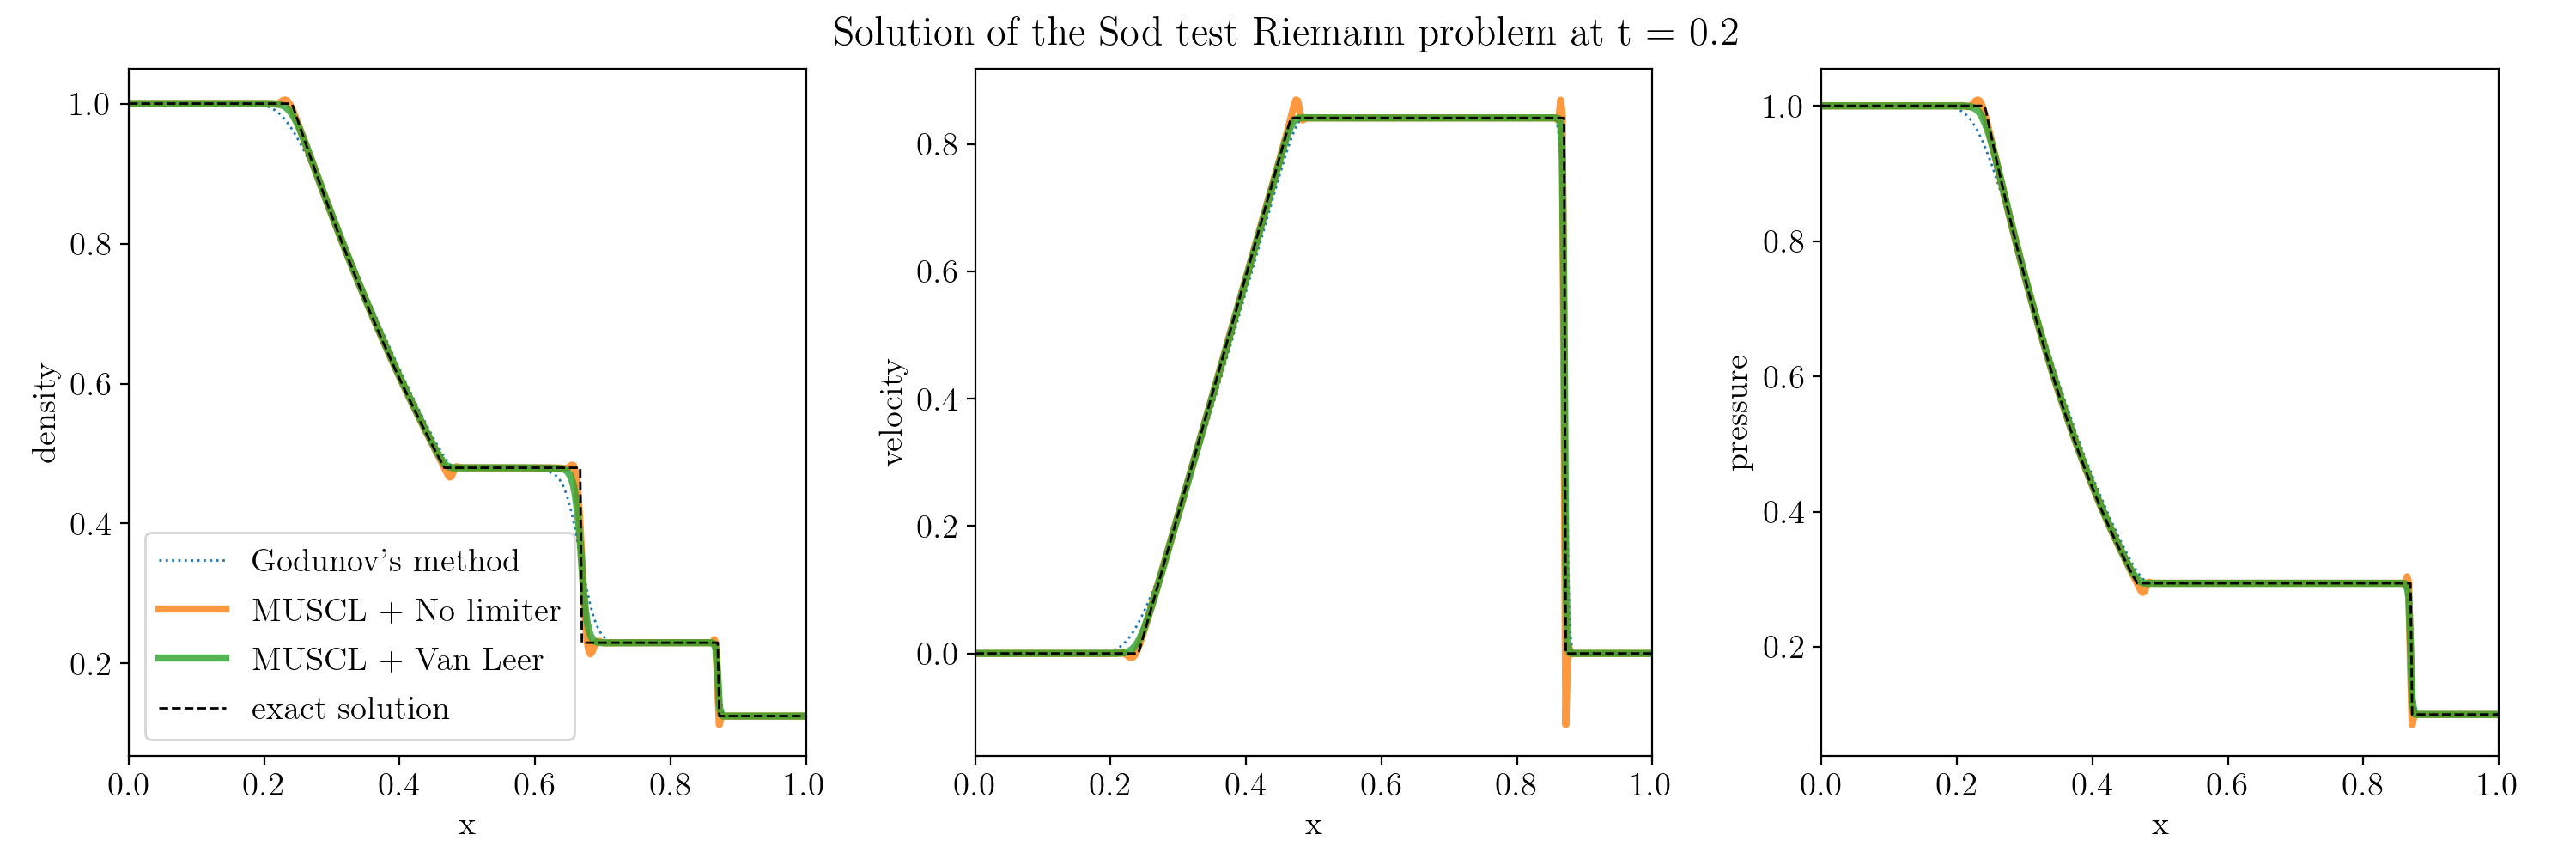
\includegraphics[width=\linewidth]{figures/FV/MUSCL-Hancock/MUSCL-comparison-sod_test-1D.png}
   \caption[Sod test using MUSCL-Hancock method]{
The solution to the Sod test (eq. \ref{eq:sod-test-ICs}) using Godunov's method, the MUSCL-Hancock
method with a limiter, and the MUSCL-Hancock method with the Van Leer limiter.
}
    \label{fig:MUSCL-sod-test}
\end{figure}
%
\begin{figure}
   \centering
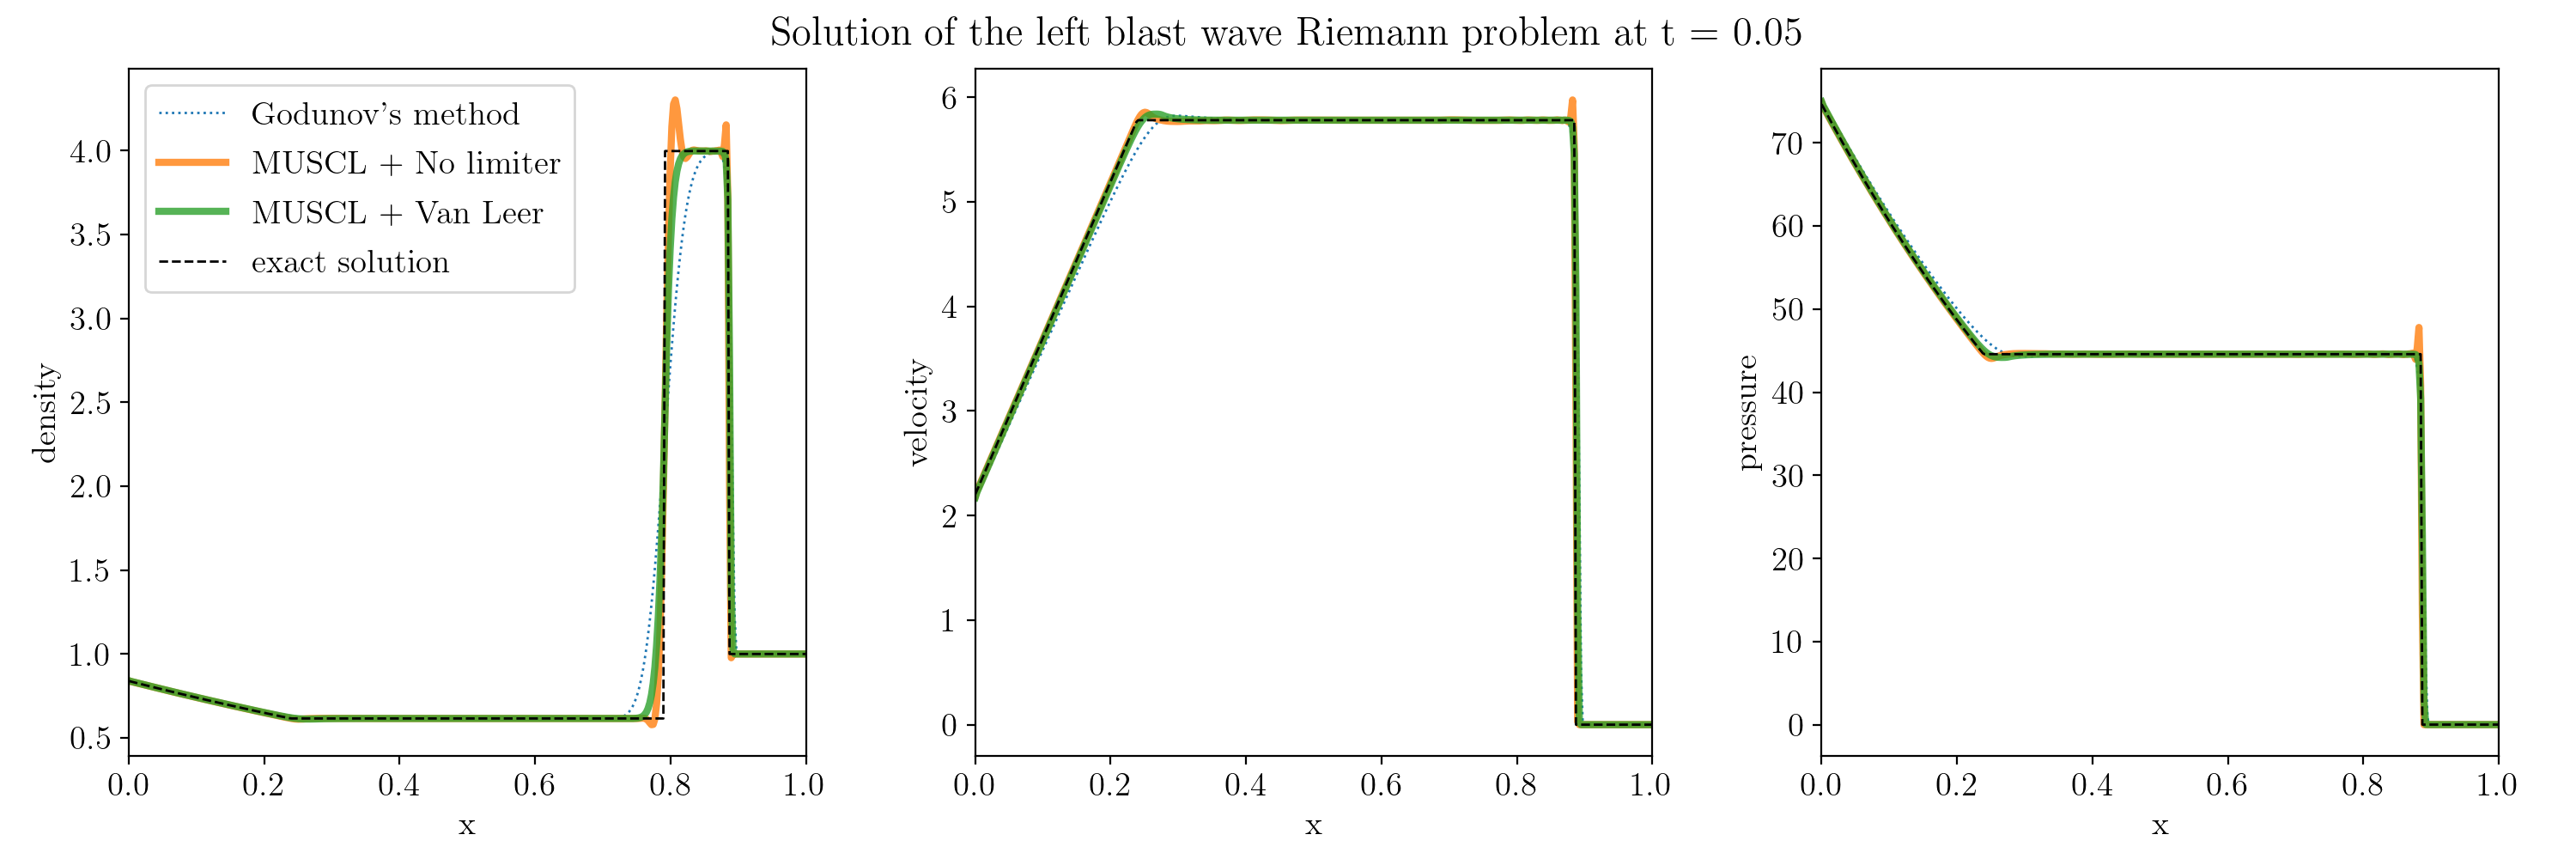
\includegraphics[width=\linewidth]{figures/FV/MUSCL-Hancock/MUSCL-comparison-left_blast_wave-1D.png}
   \caption[Left Blast Wave test using MUSCL-Hancock method]{
The solution to the Left Blast Wave test (eq. \ref{eq:left-blast-wave-ICs}) using Godunov's method,
the MUSCL-Hancock method with a limiter, and the MUSCL-Hancock method with the Van Leer limiter.
}
   \label{fig:MUSCL-left-blast-wave}
\end{figure}
%
\begin{figure}
   \centering
   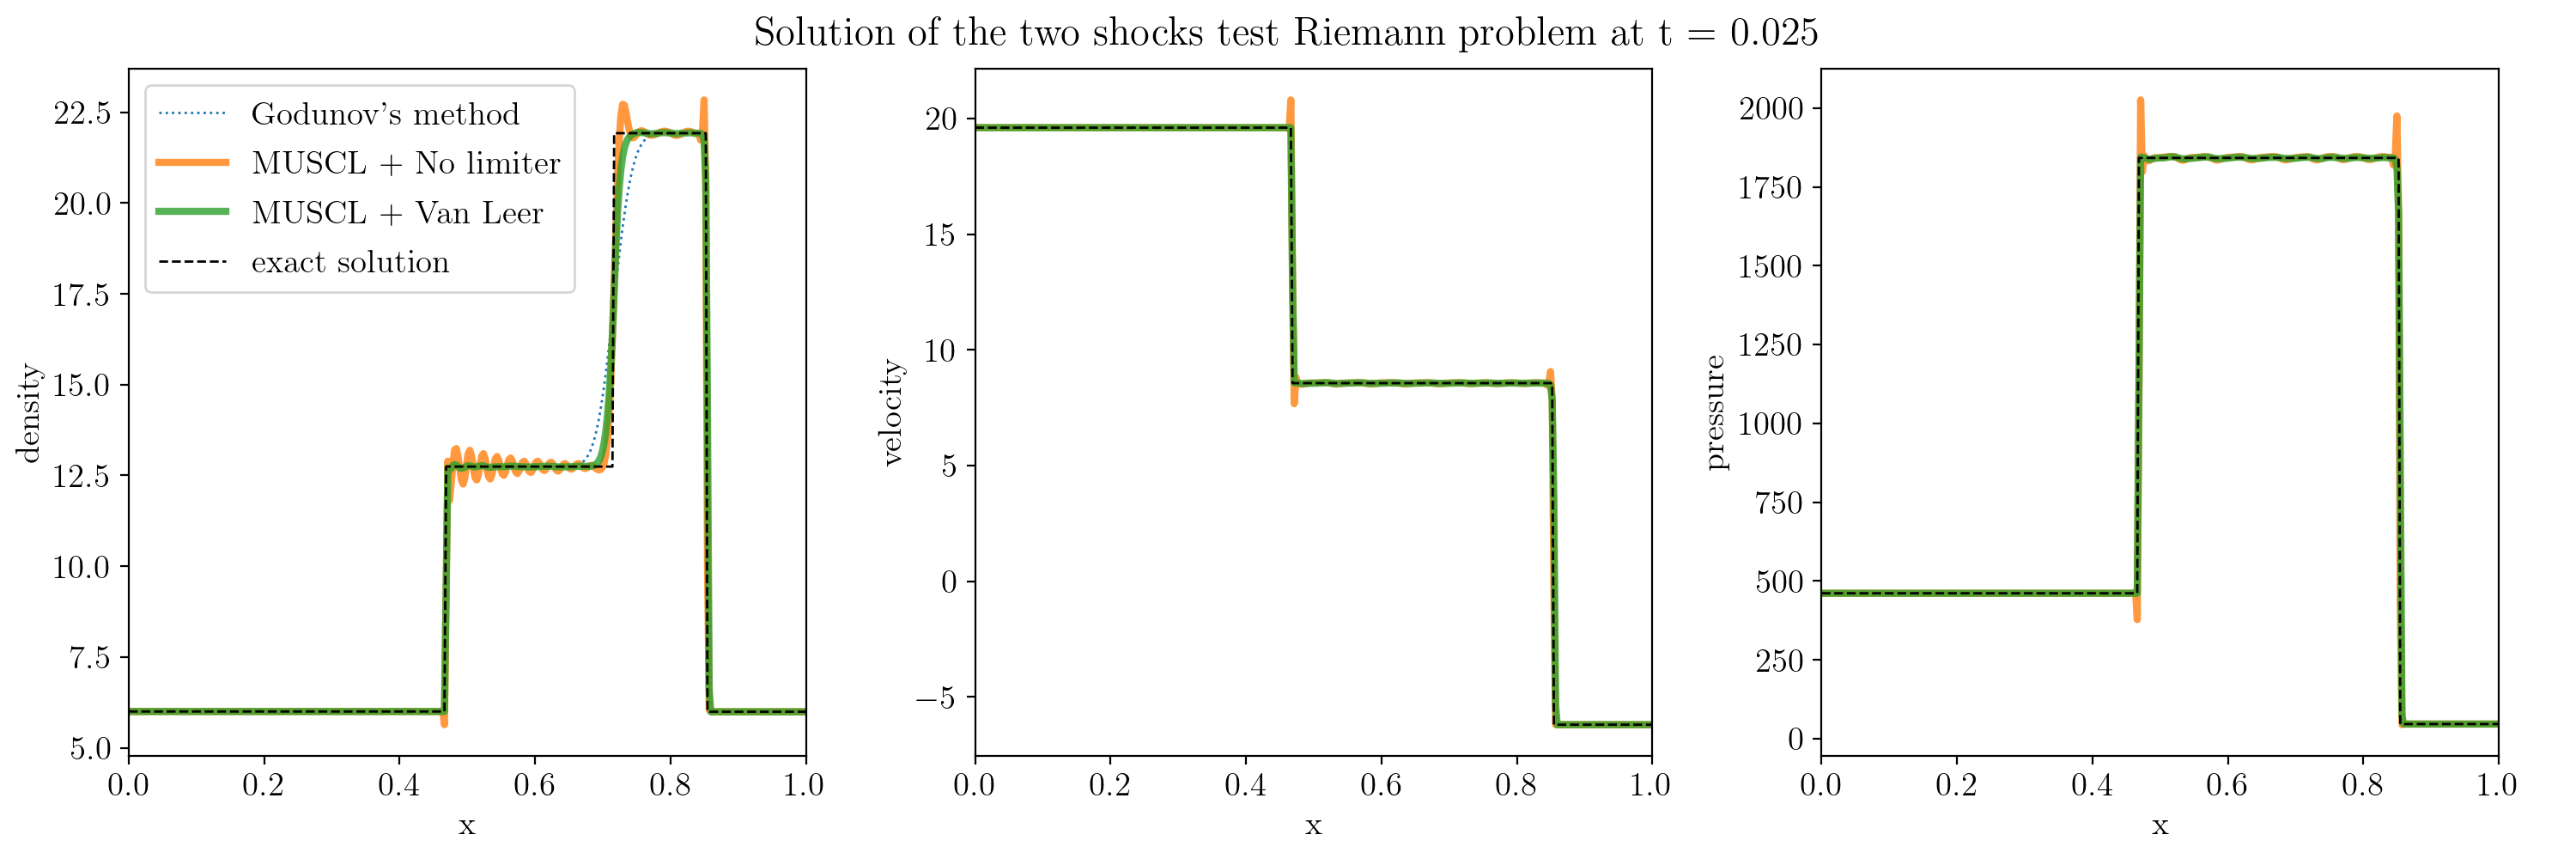
\includegraphics[width=\linewidth]{figures/FV/MUSCL-Hancock/MUSCL-comparison-two_shocks-1D.png}
   \caption[Two Shocks test using MUSCL-Hancock method]{
The solution to the Two Shocks test (eq. \ref{eq:two-shock-ICs}) using Godunov's method, the
MUSCL-Hancock method with a limiter, and the MUSCL-Hancock method with the Van Leer limiter.
}
    \label{fig:MUSCL-two-shocks}
\end{figure}





\begin{figure}
\centering
\includegraphics[width=.5\linewidth]{figures/FV/godunov_euler/kelvin-helmholtz-0000.png}%
\includegraphics[width=.5\linewidth]{figures/FV/MUSCL-Hancock/kelvin-helmholtz-0000.png}%
\\
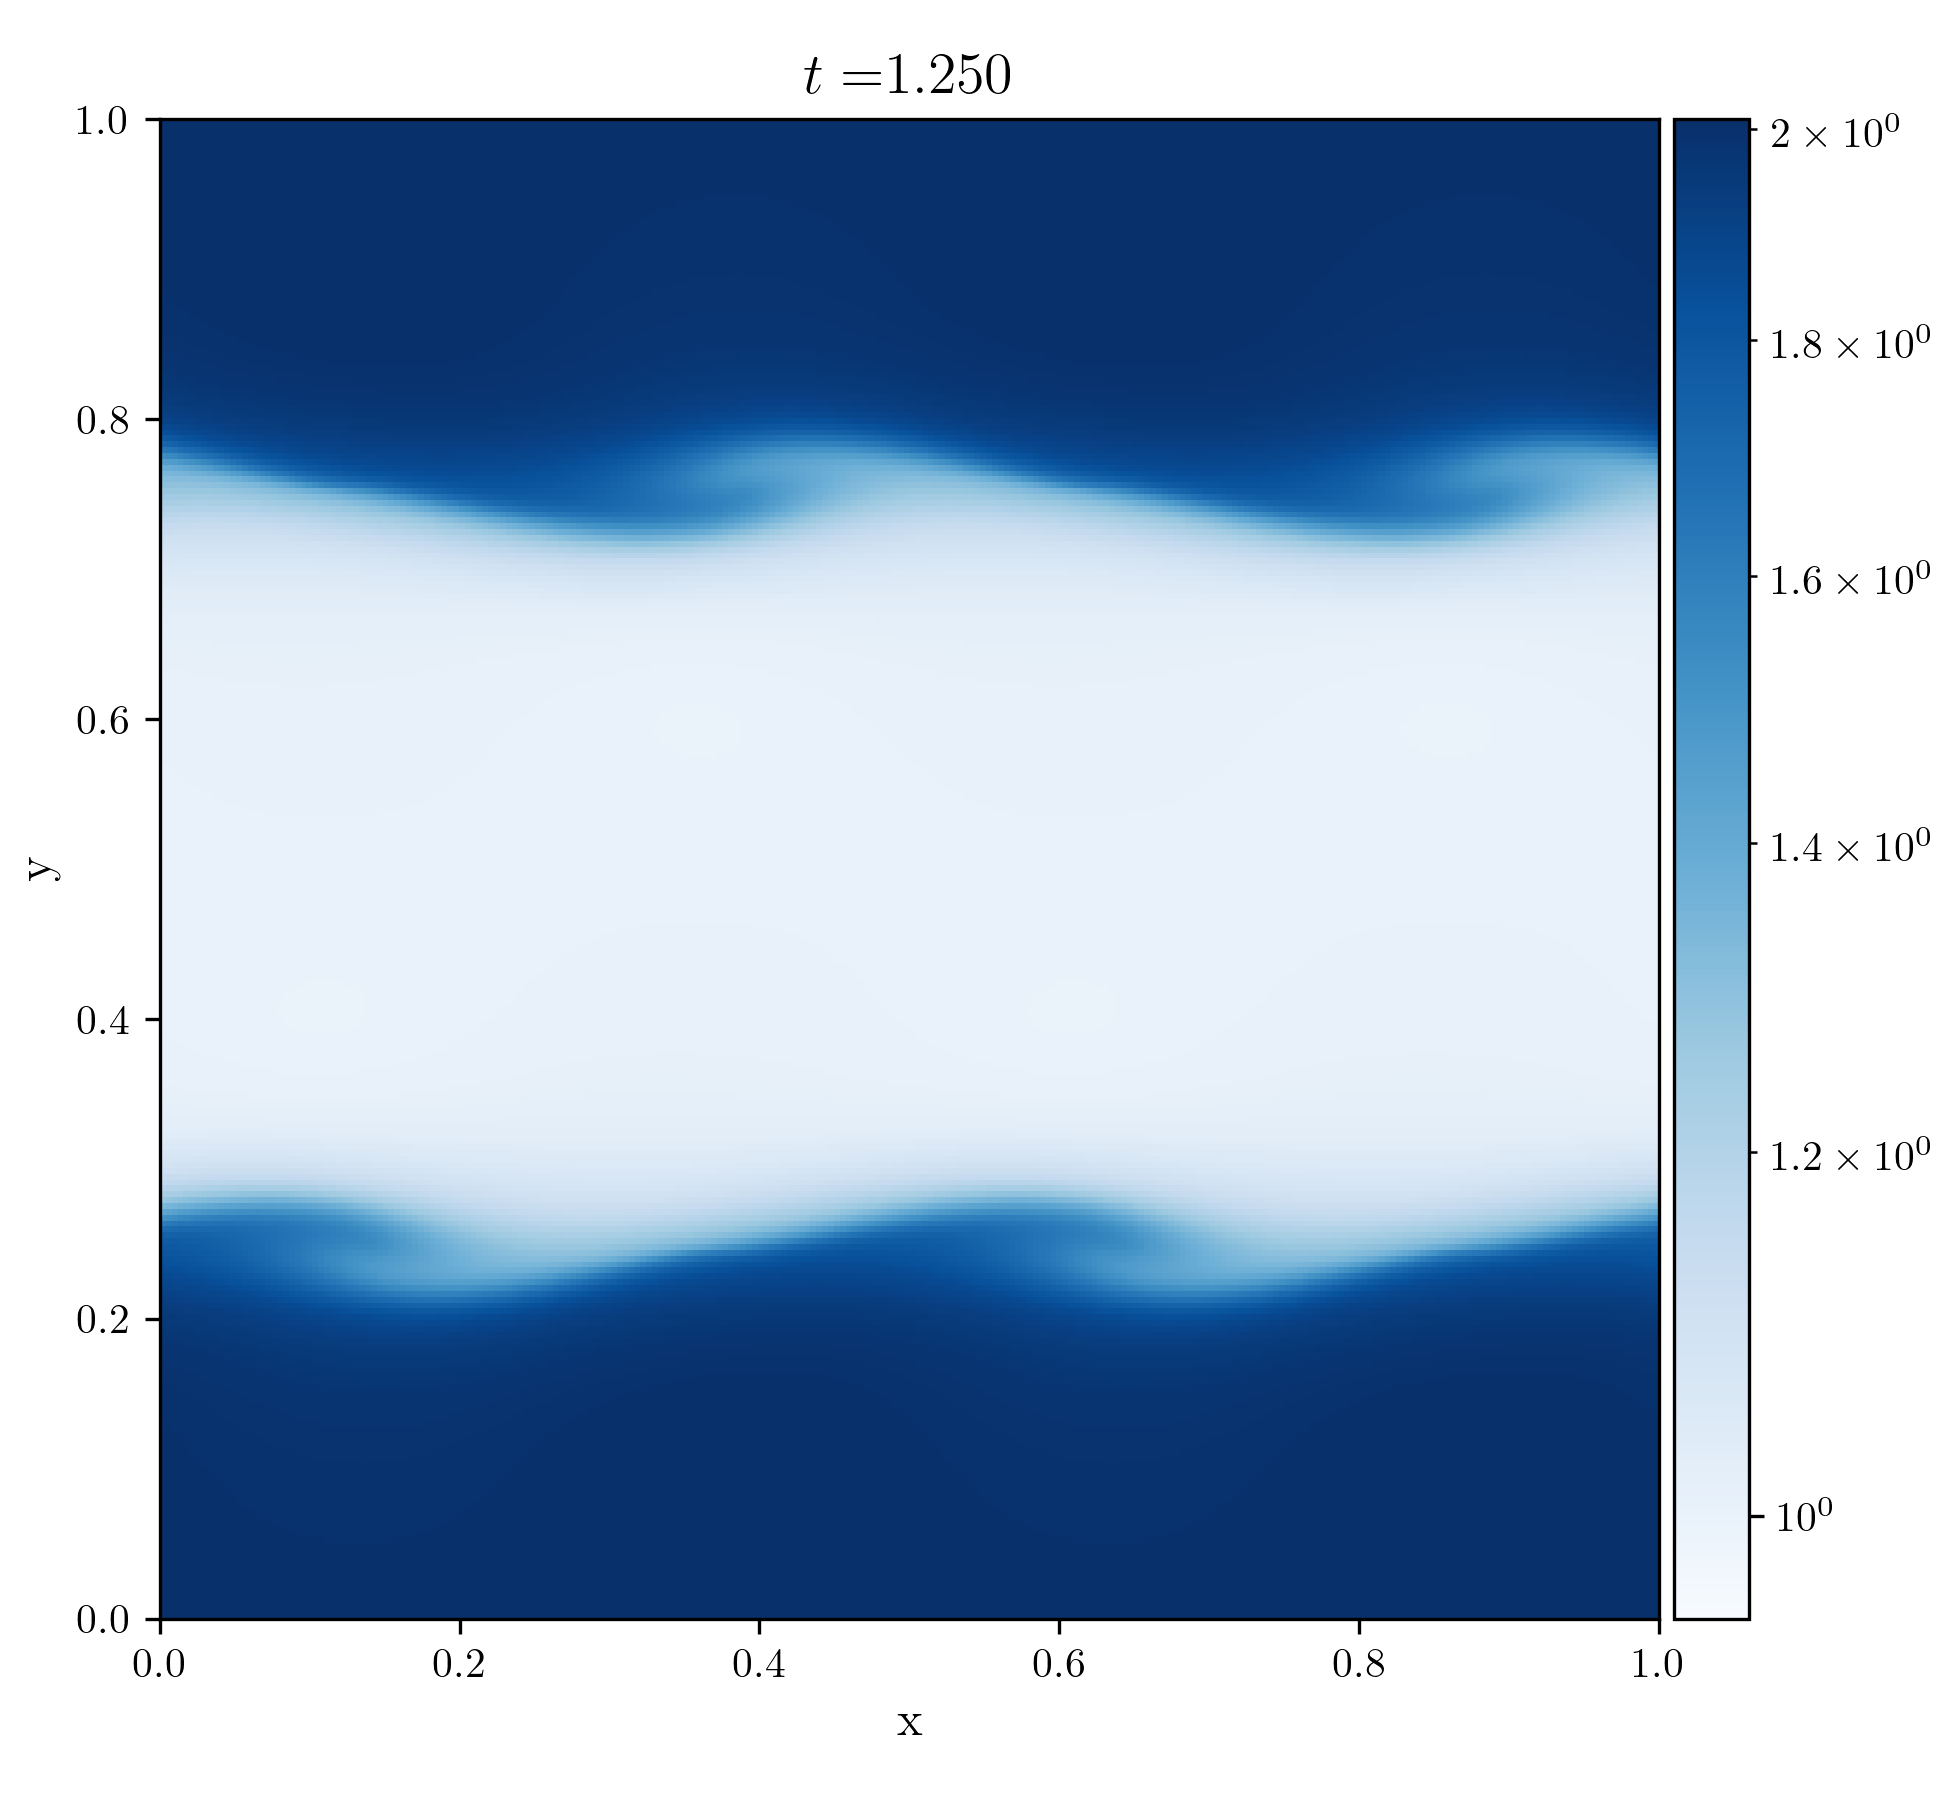
\includegraphics[width=.5\linewidth]{figures/FV/godunov_euler/kelvin-helmholtz-0250.png}%
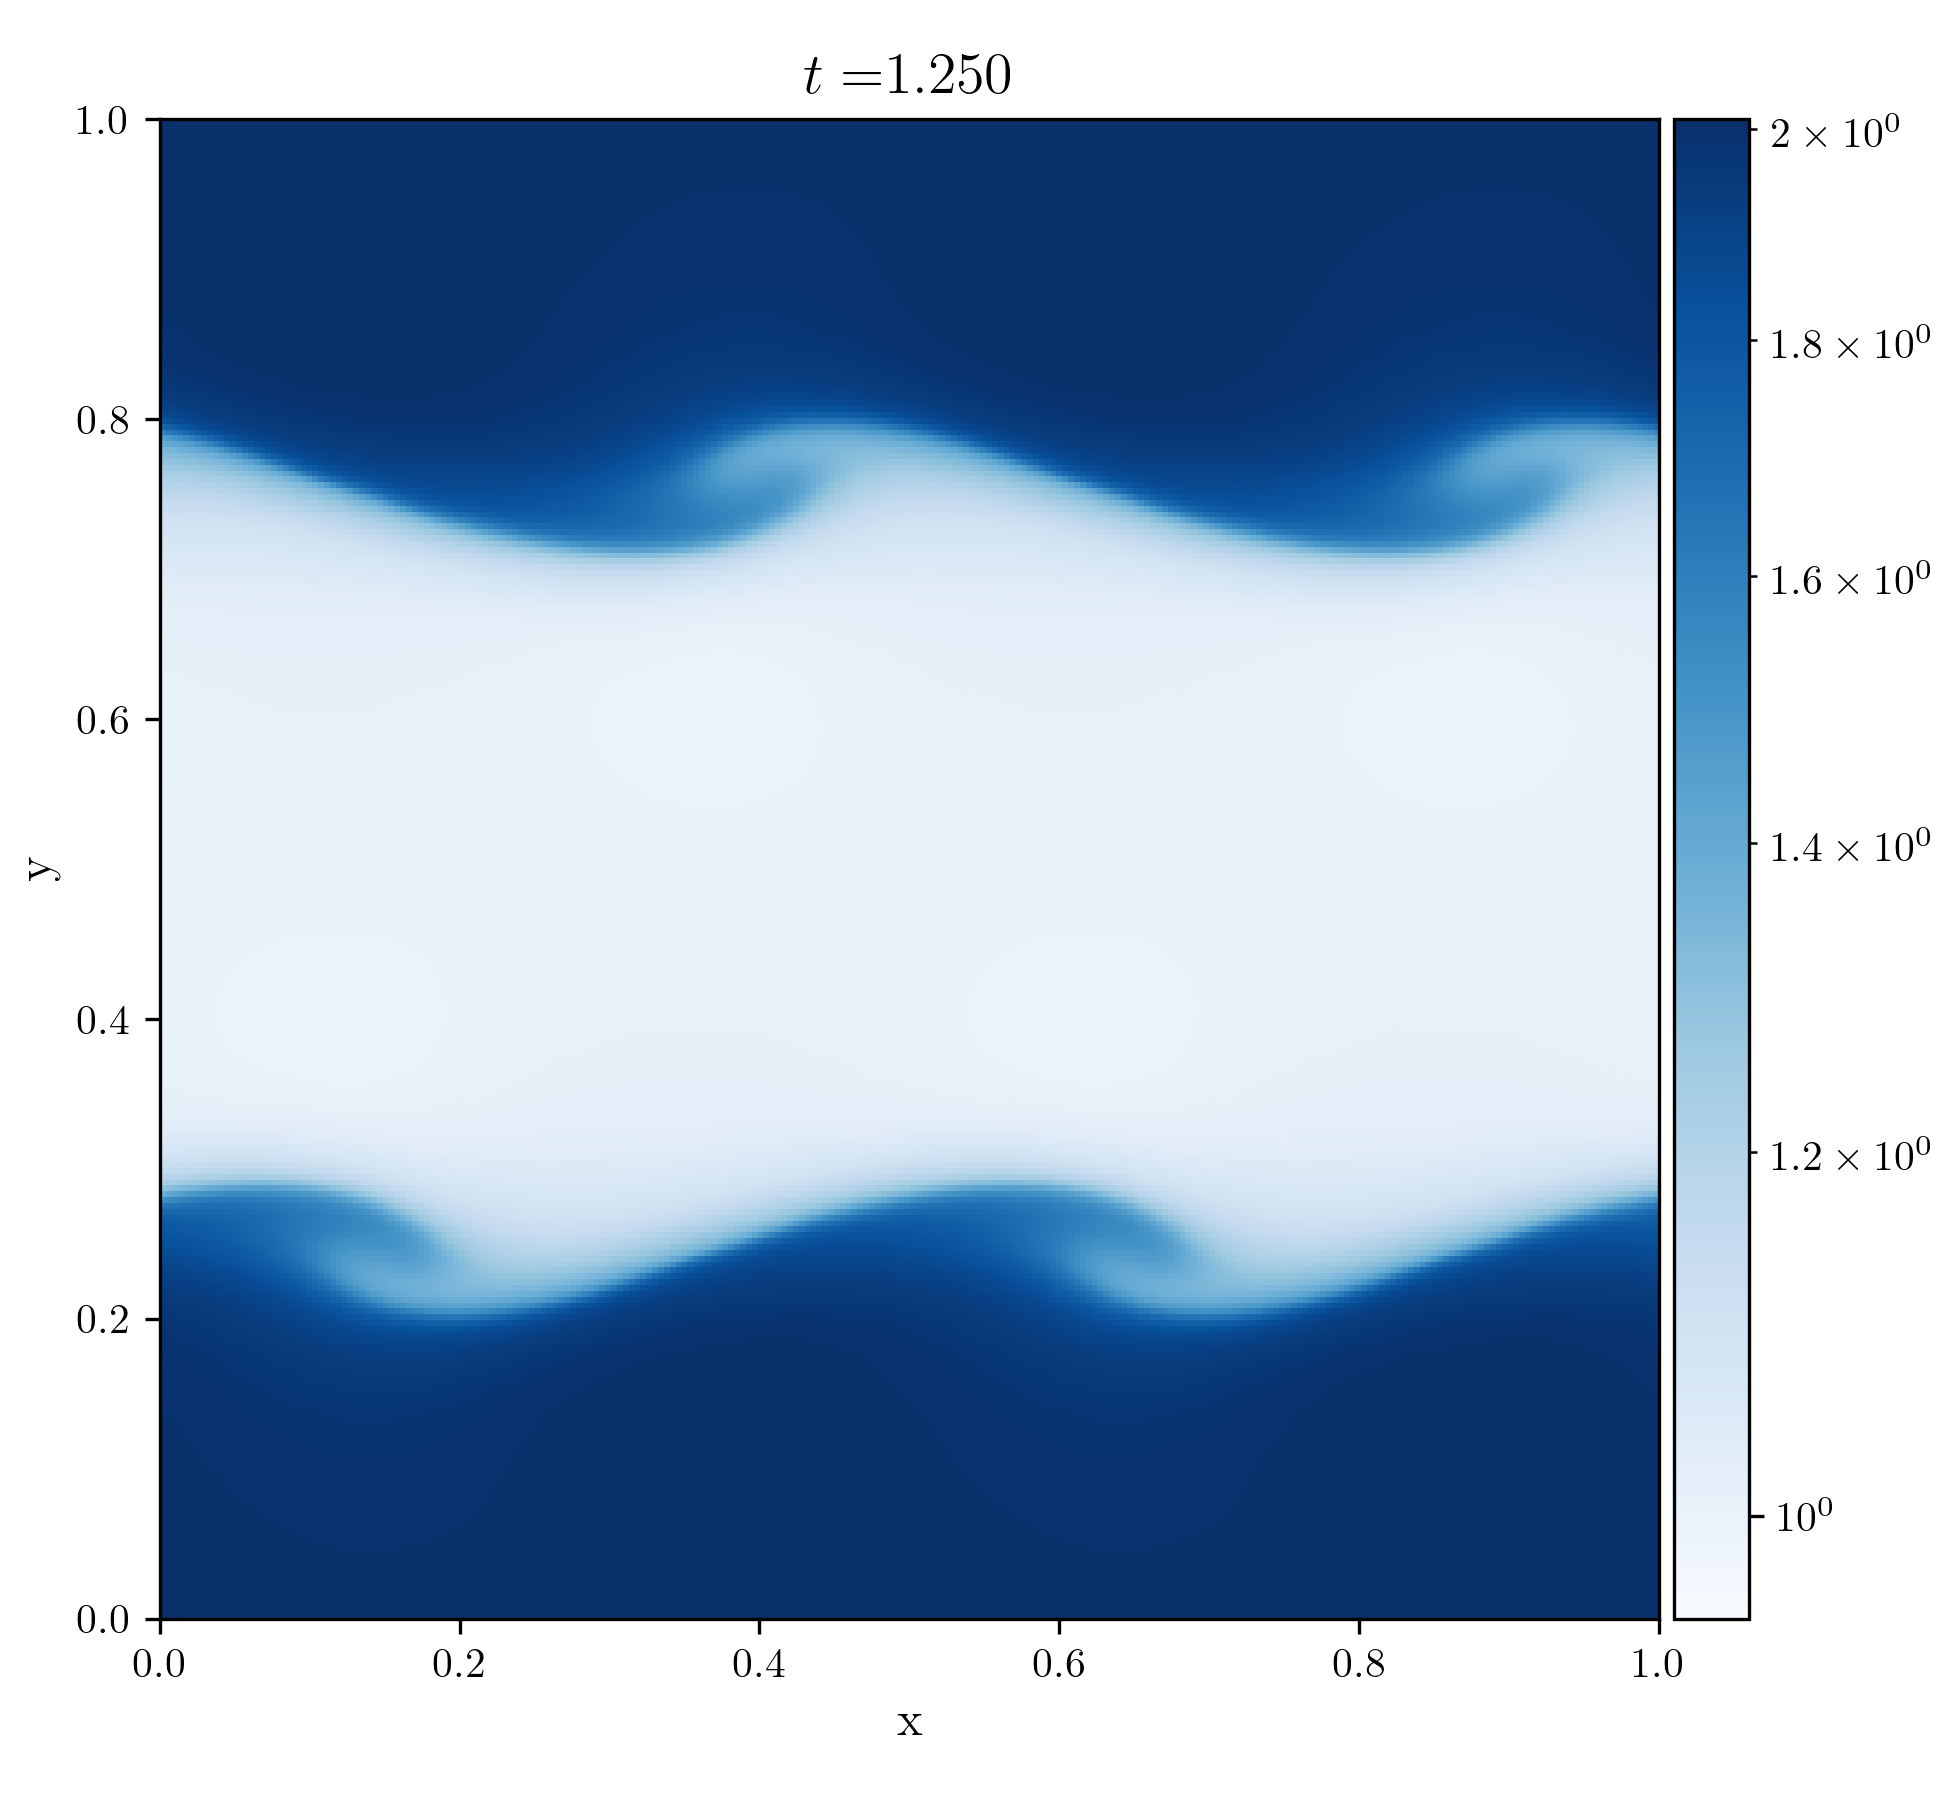
\includegraphics[width=.5\linewidth]{figures/FV/MUSCL-Hancock/kelvin-helmholtz-0250.png}%
\\
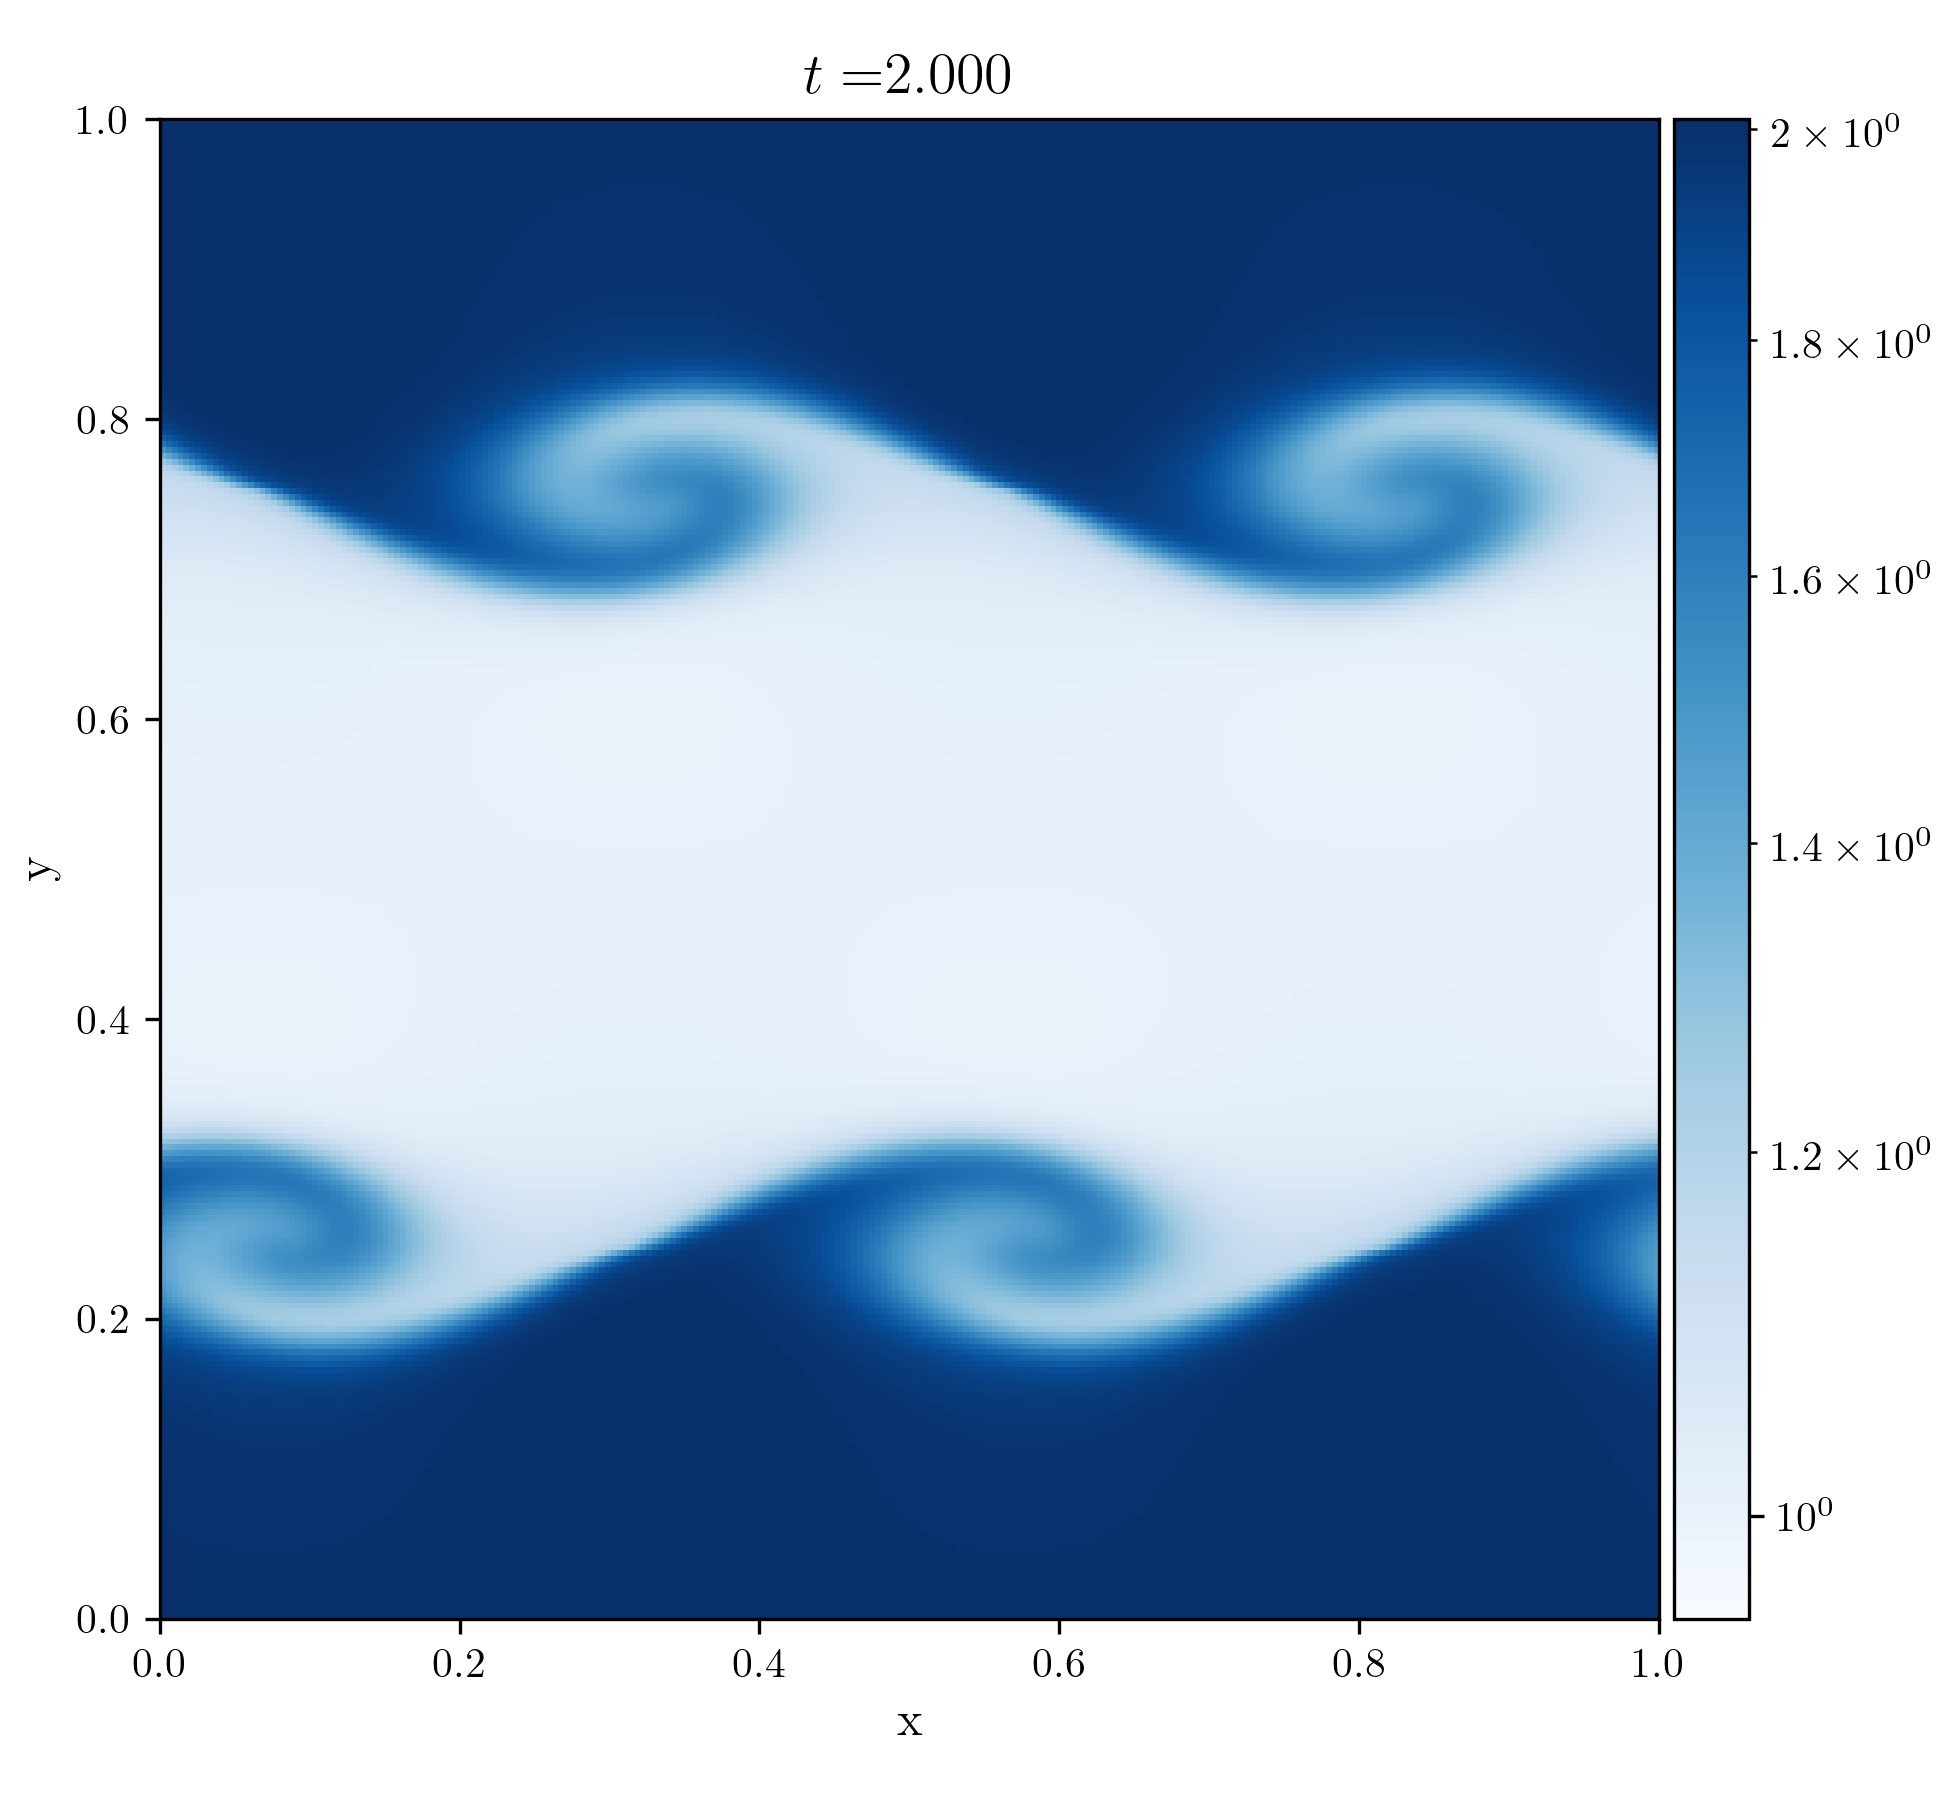
\includegraphics[width=.5\linewidth]{figures/FV/godunov_euler/kelvin-helmholtz-0400.png}%
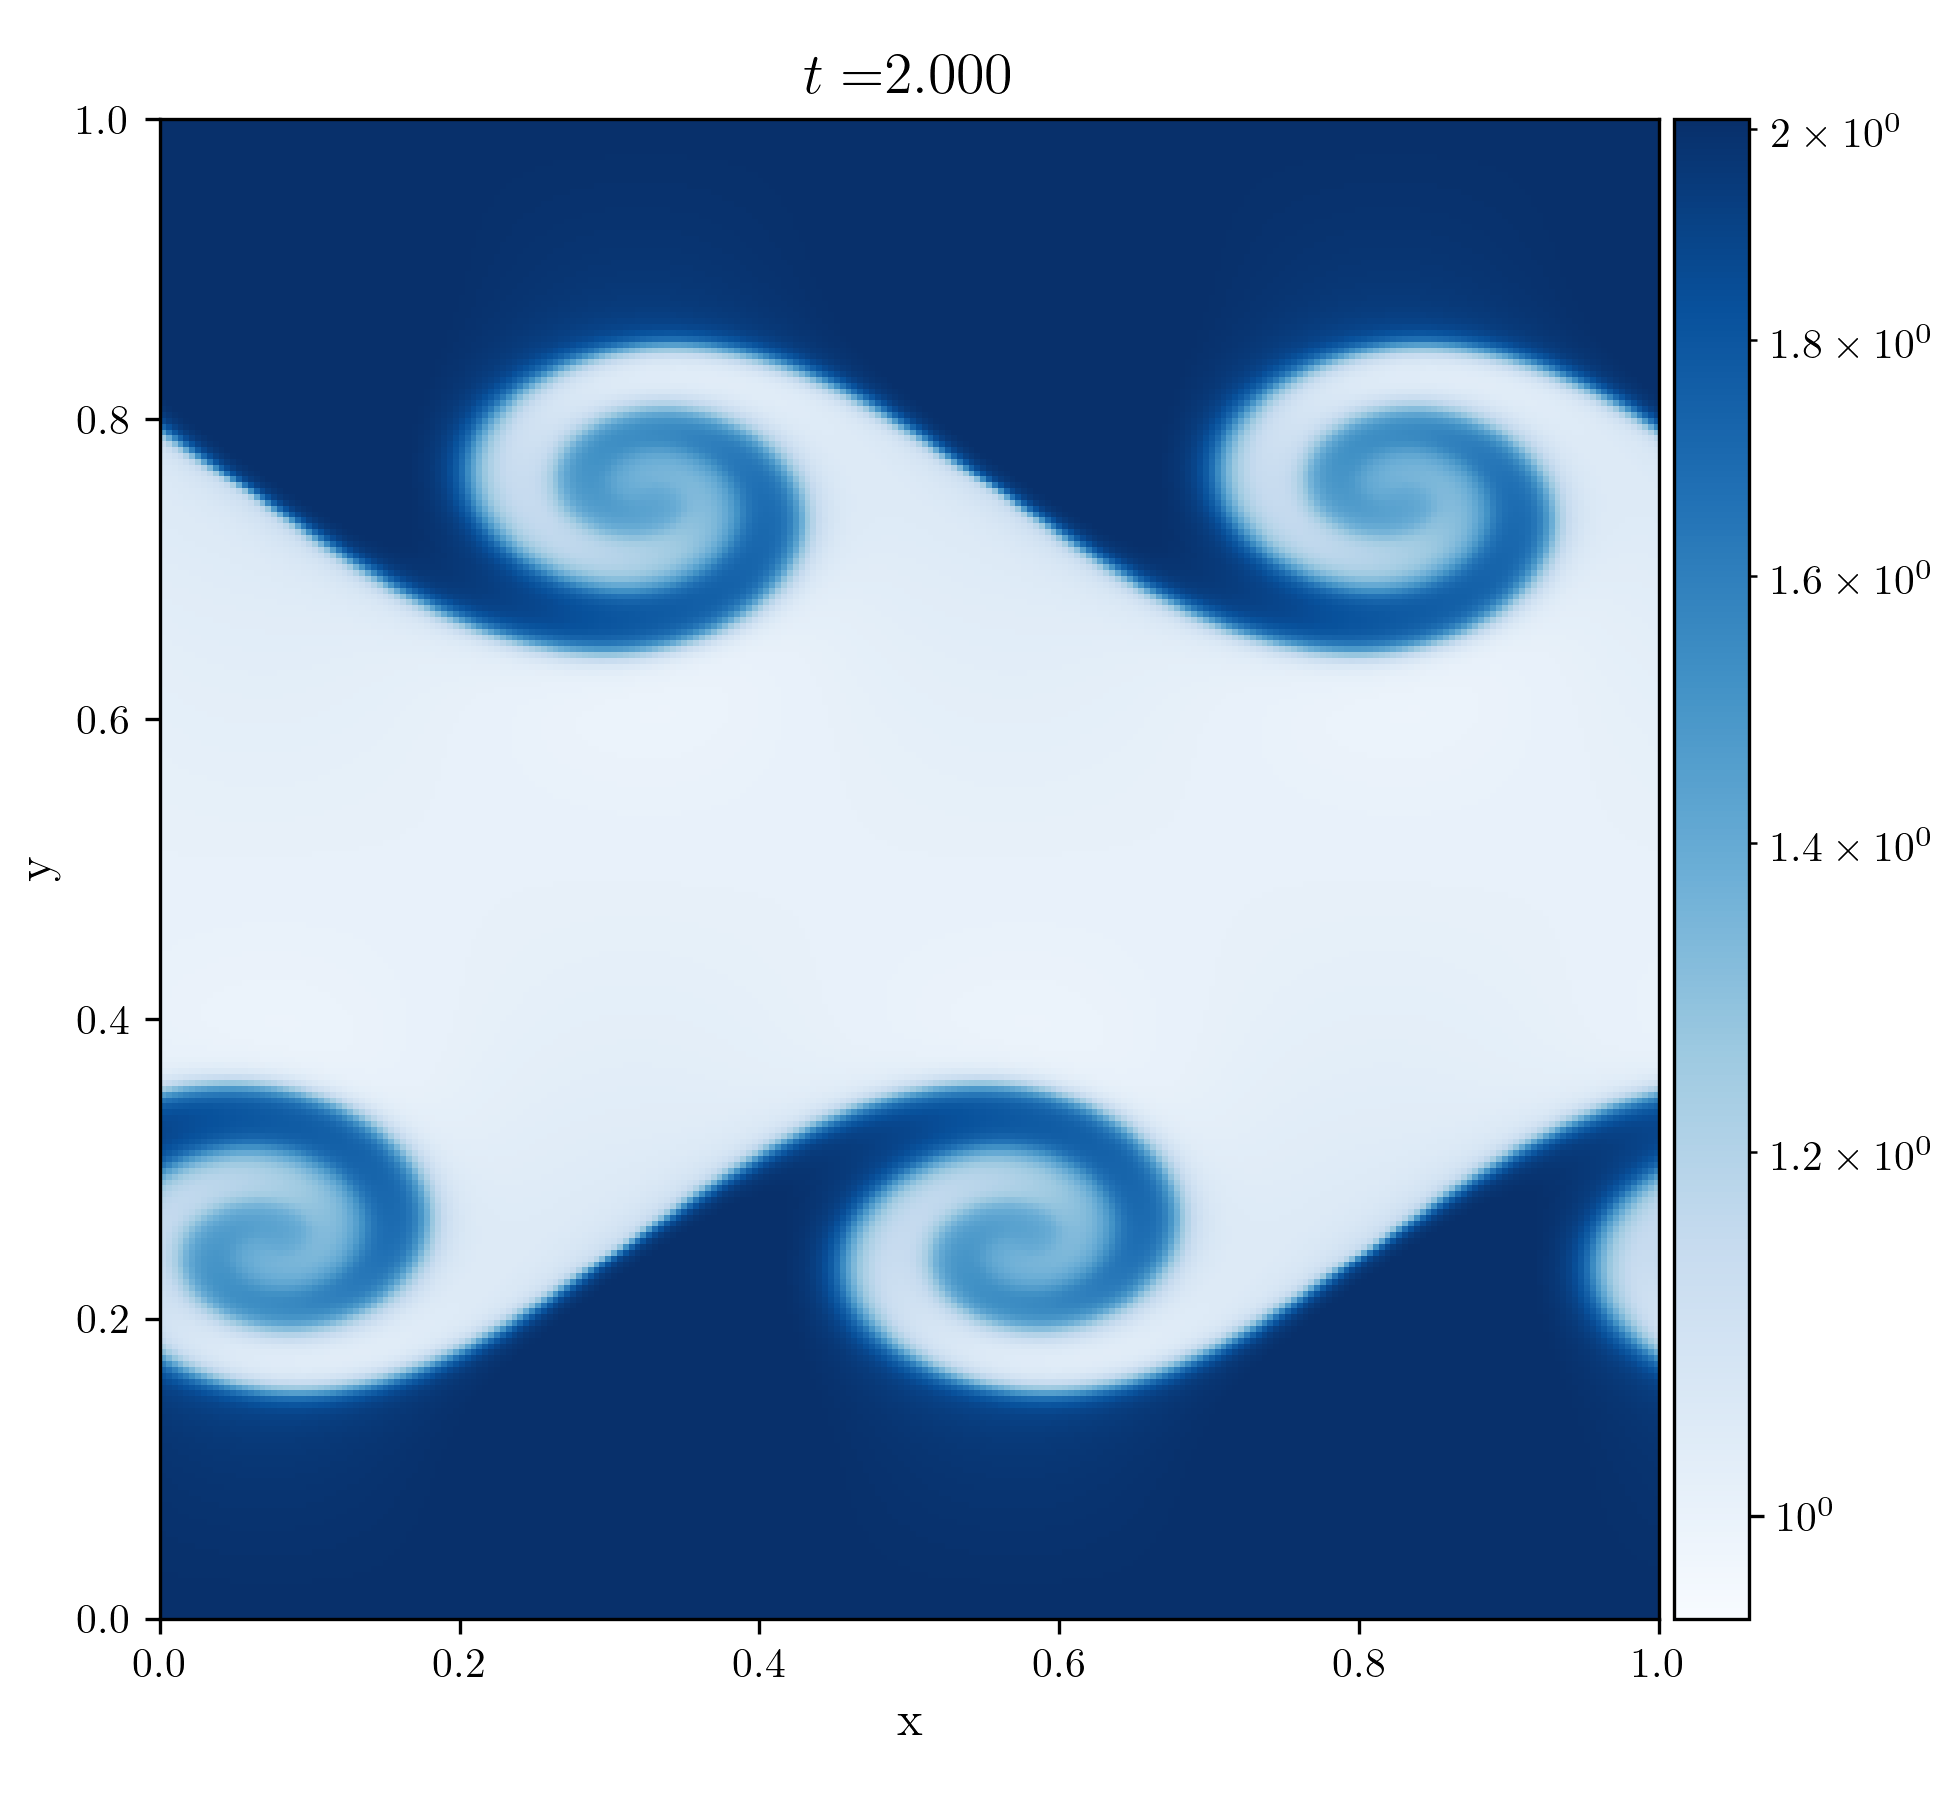
\includegraphics[width=.5\linewidth]{figures/FV/MUSCL-Hancock/kelvin-helmholtz-0400.png}%
\caption[Kelvin-Helmholtz Instability with Godunov's scheme and MUSCL-Hancock 1]{
Density evolution for the Kelvin-Helmholtz instability problem solved with Godunov's method (left)
and the MUSCL-Hancock method (right) at times $t = 0, 1.25, 2$ in arbitrary units.
}
\label{fig:kelvin-helmholtz-1}
\end{figure}



\begin{figure}
\centering
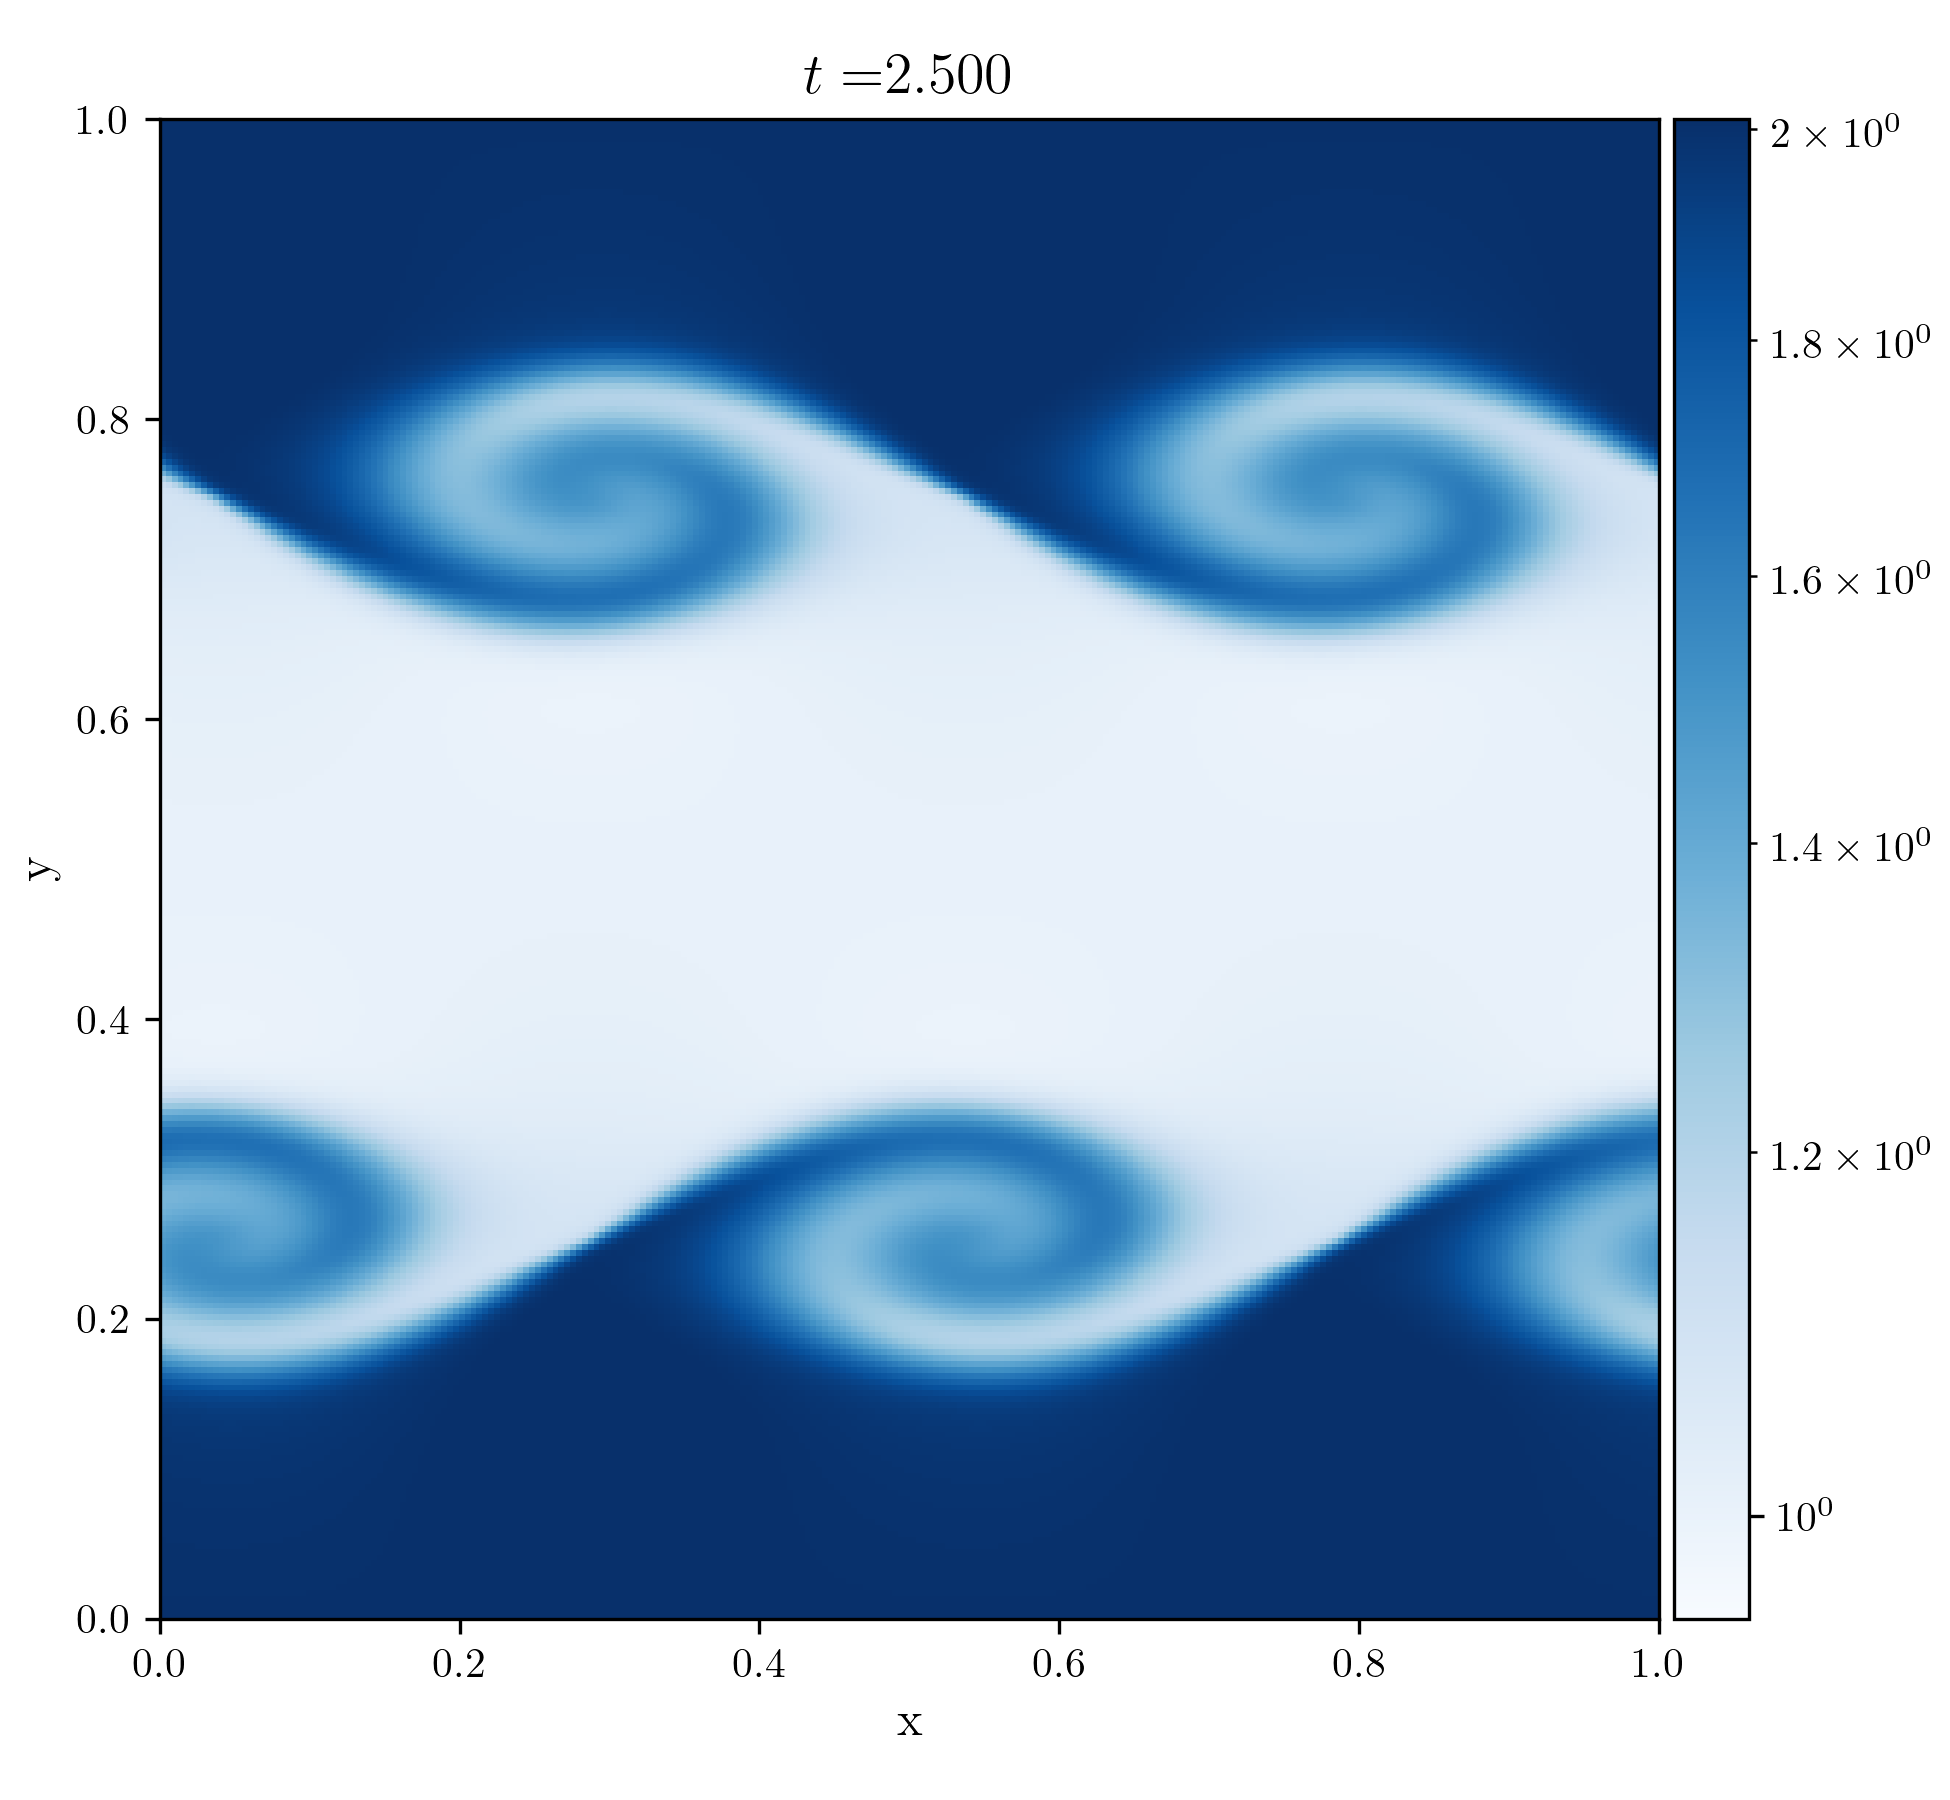
\includegraphics[width=.5\linewidth]{figures/FV/godunov_euler/kelvin-helmholtz-0500.png}%
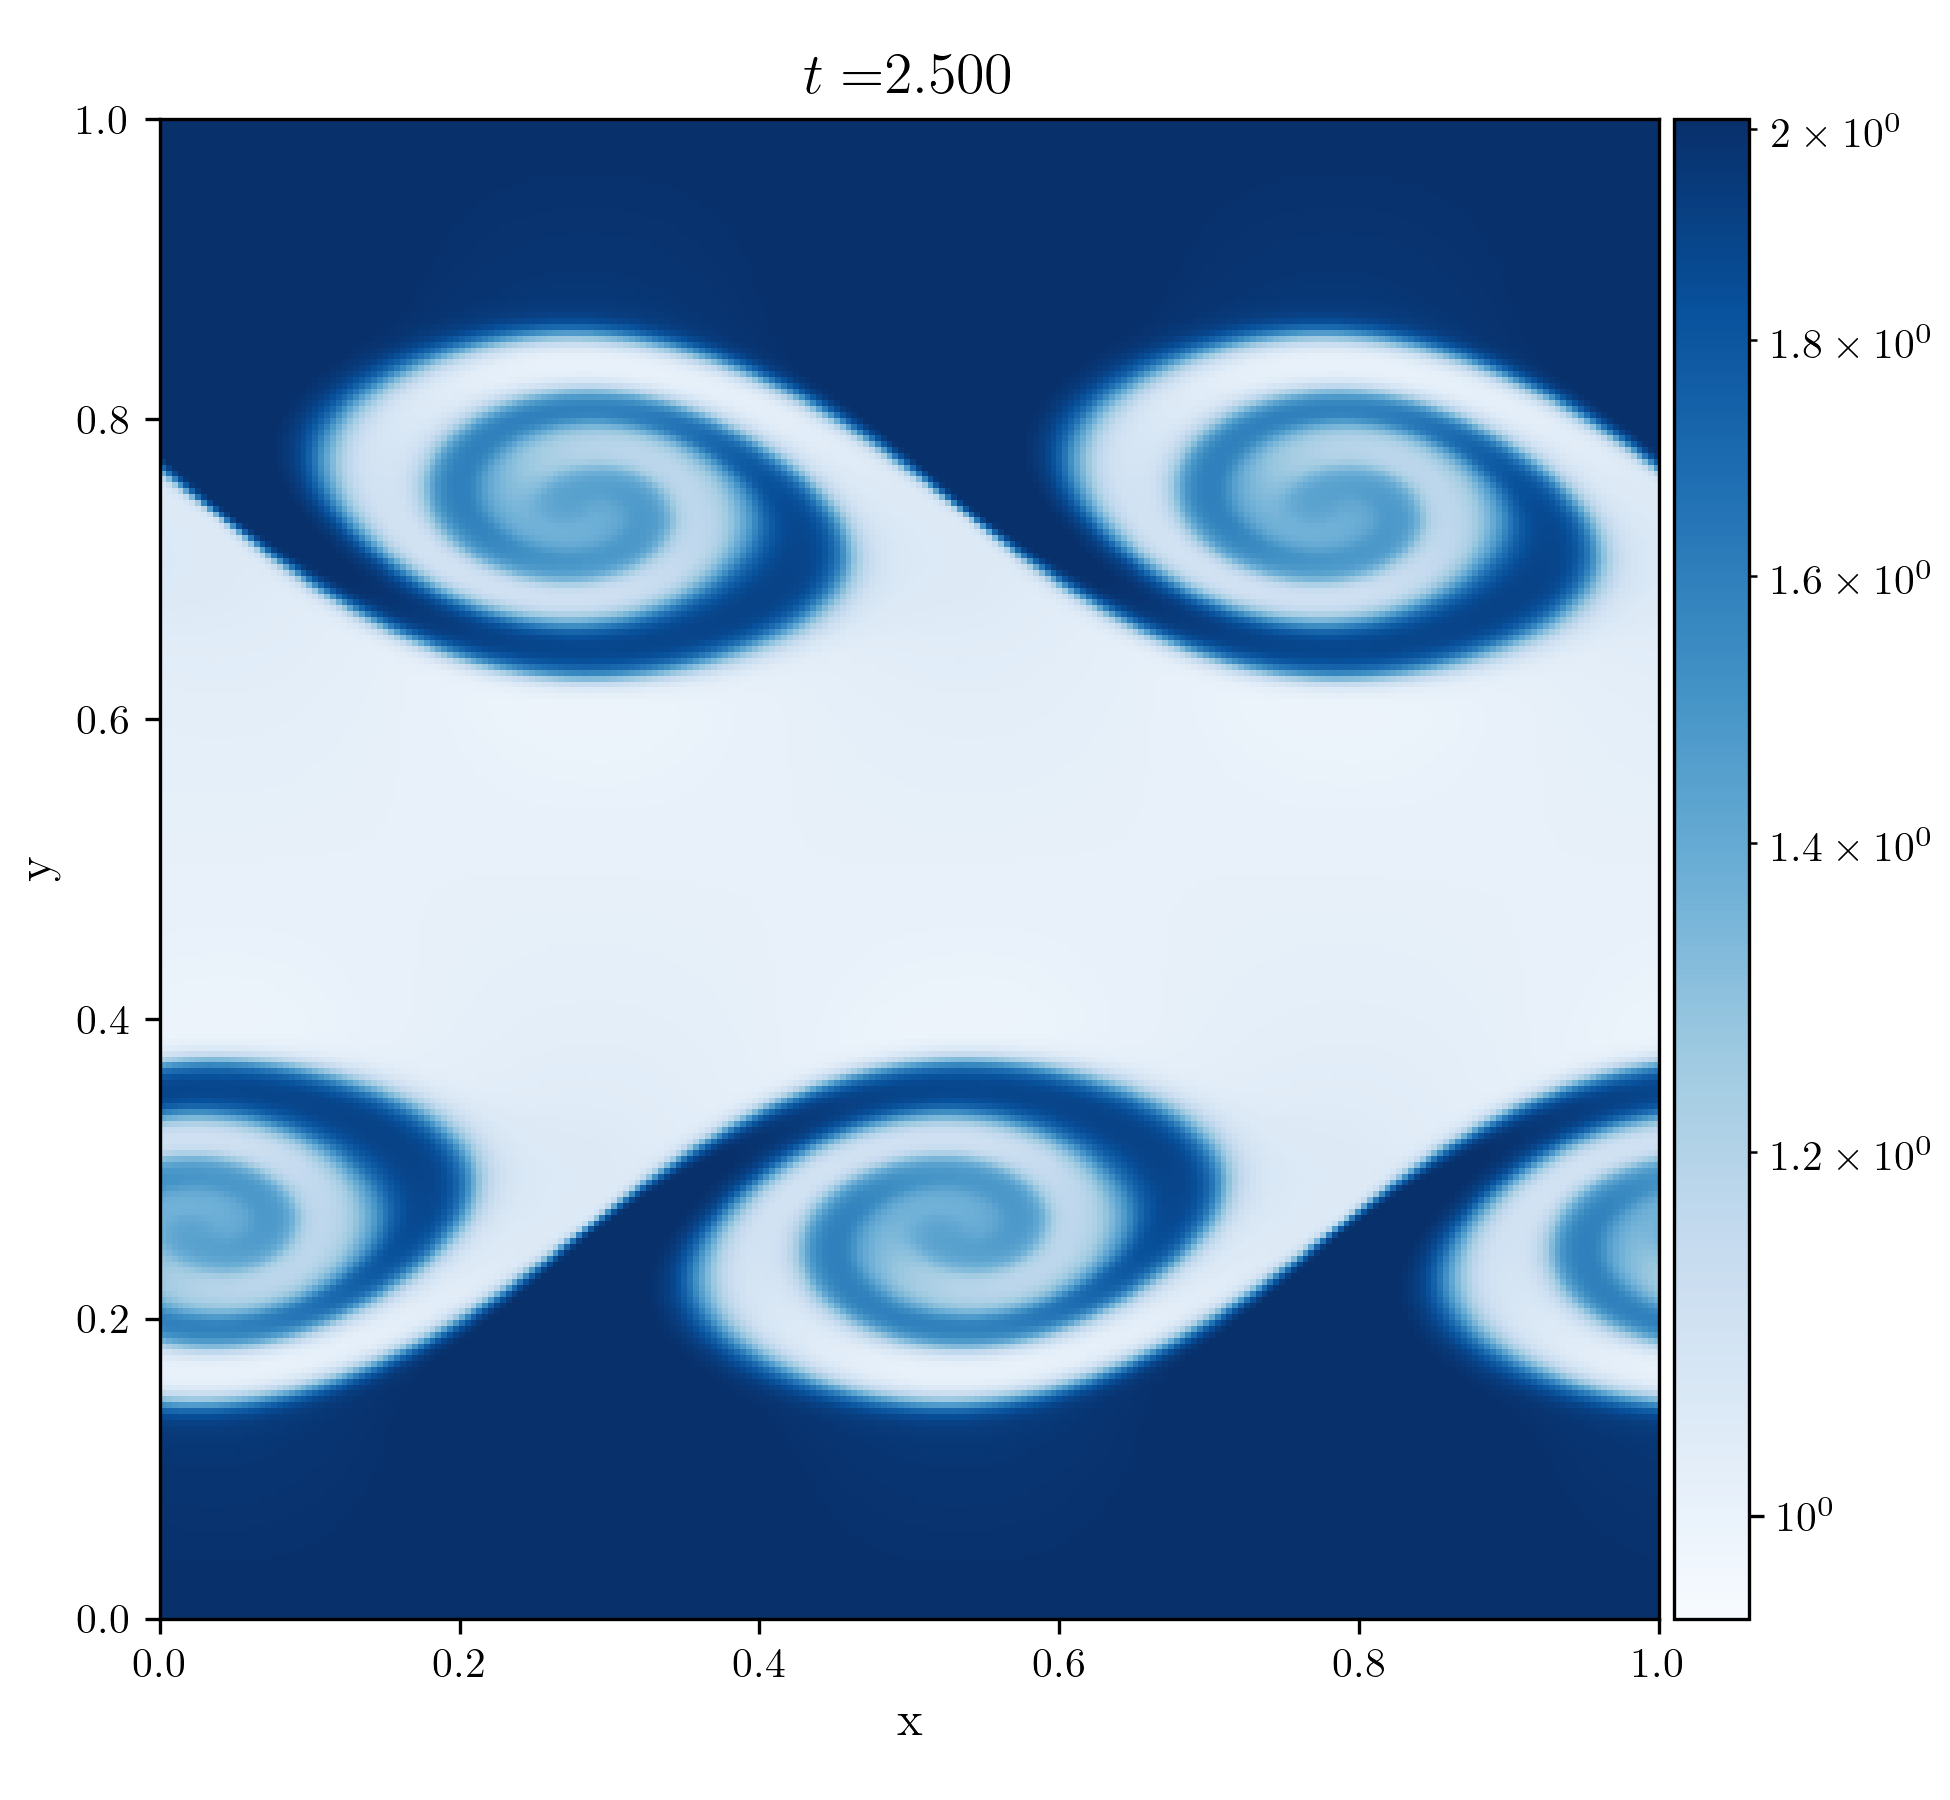
\includegraphics[width=.5\linewidth]{figures/FV/MUSCL-Hancock/kelvin-helmholtz-0500.png}%
\\
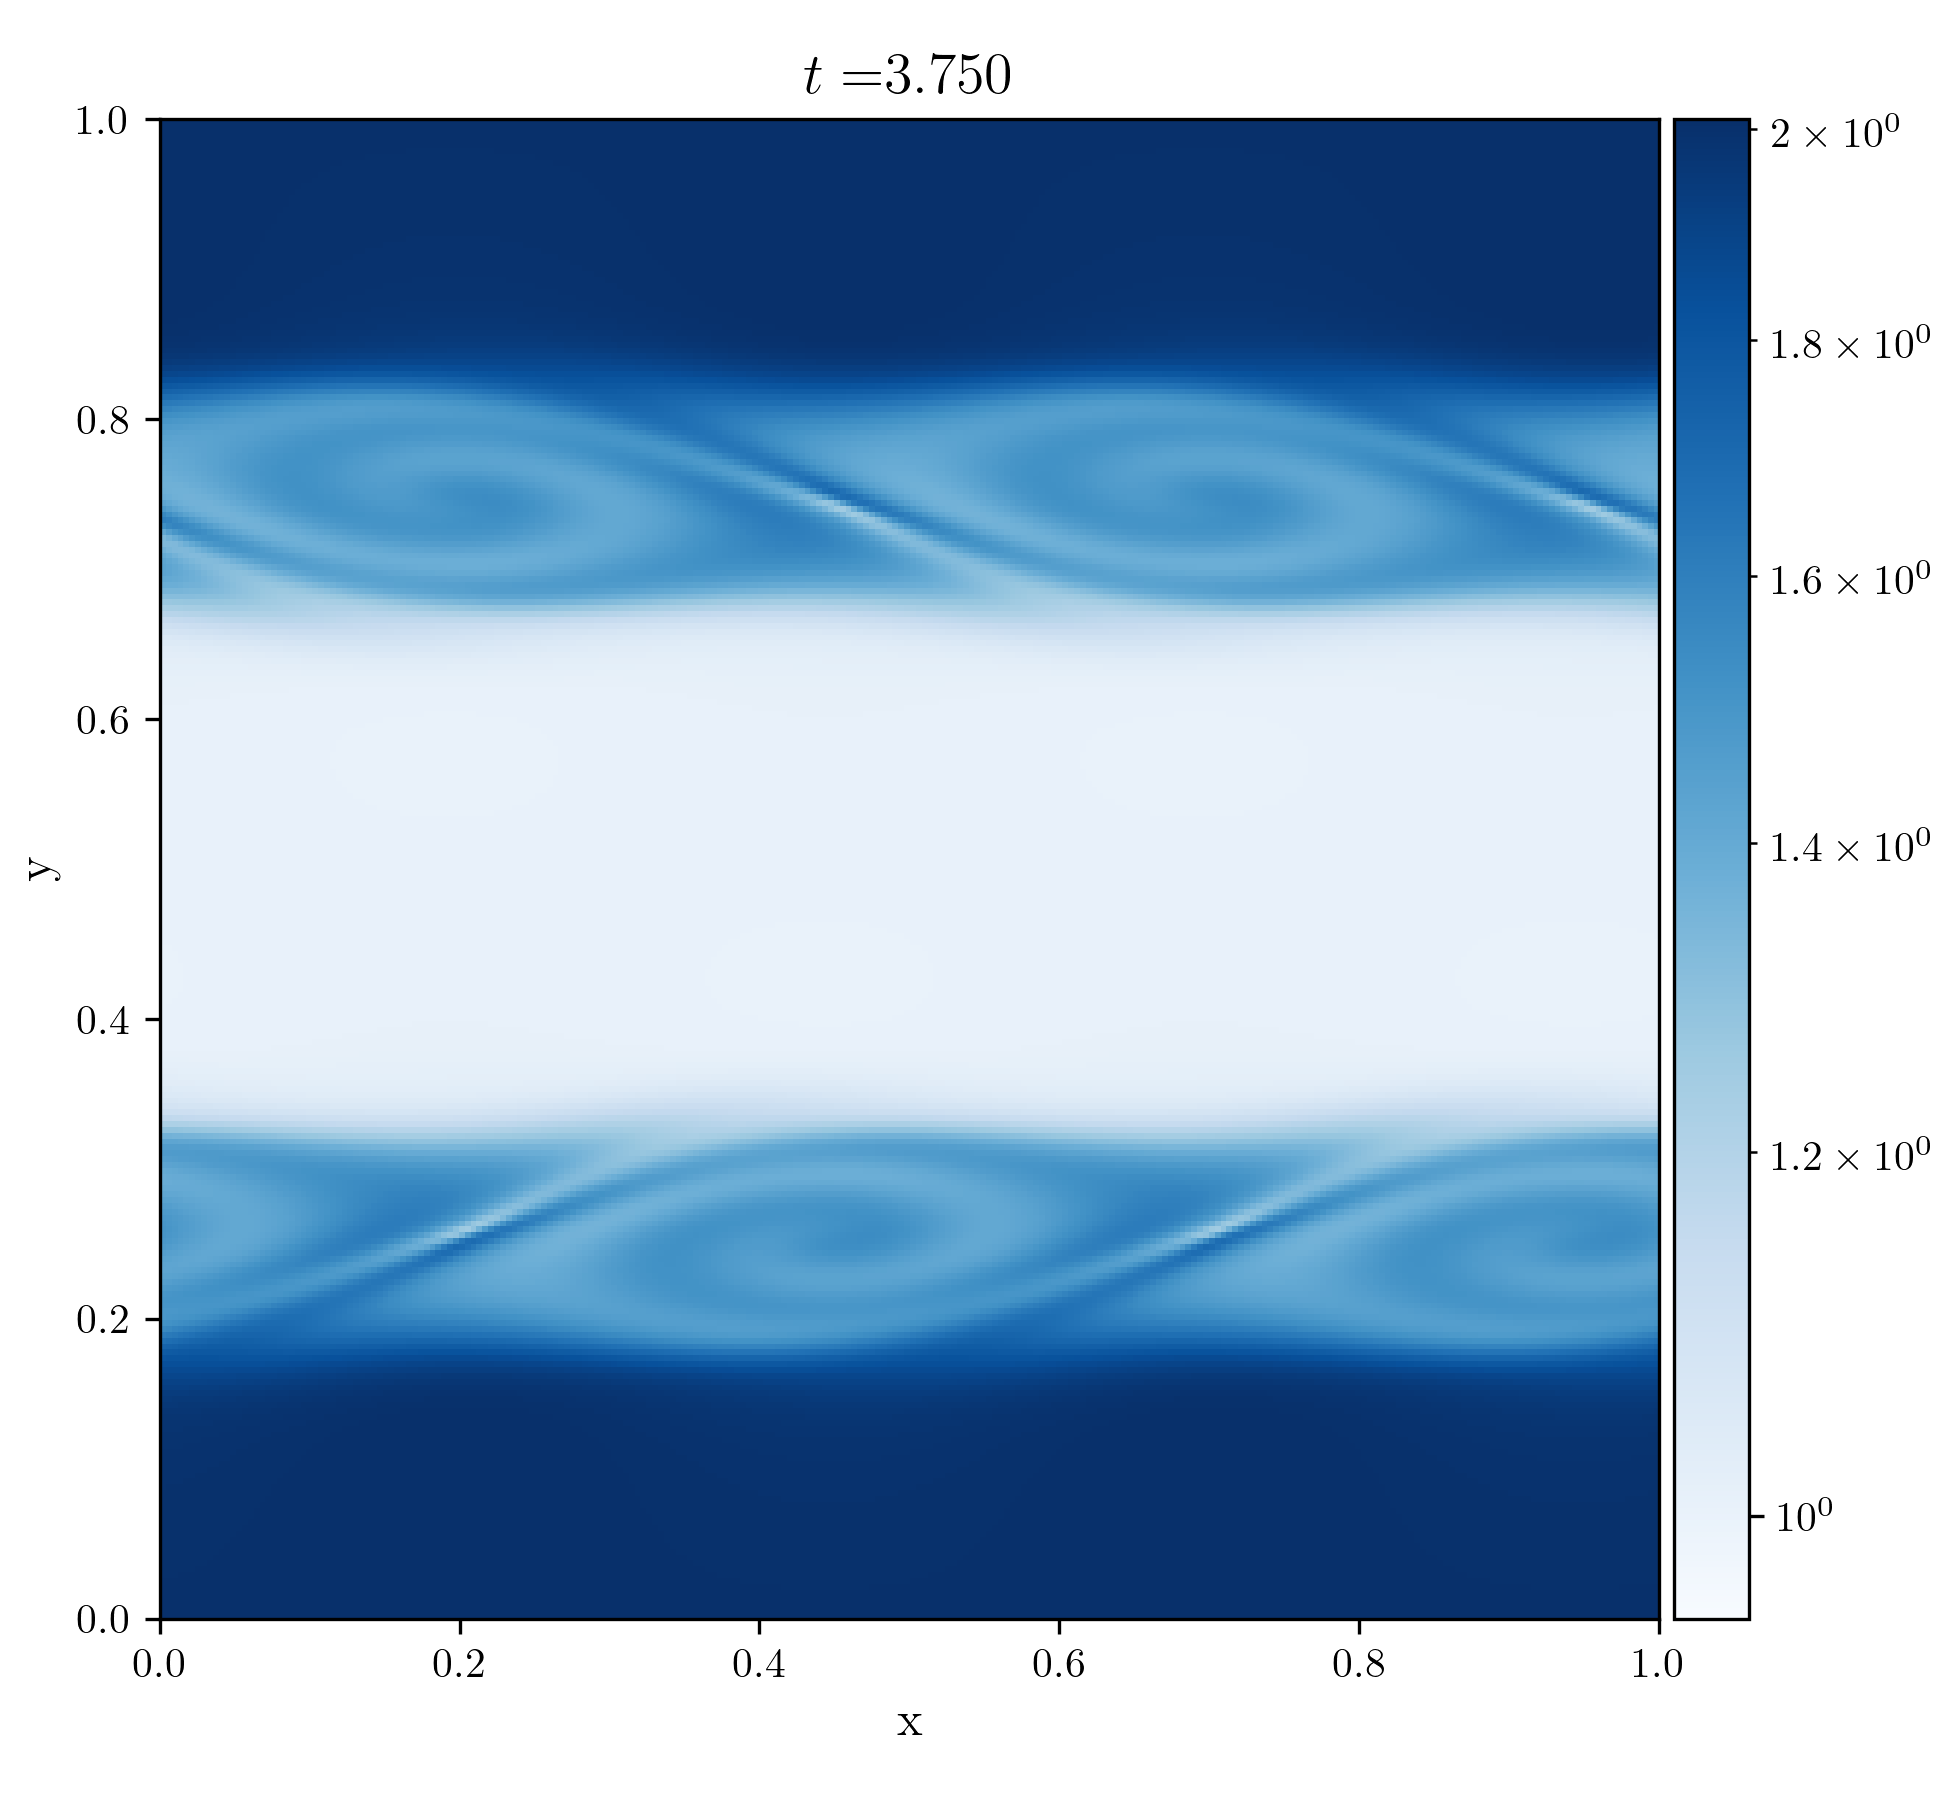
\includegraphics[width=.5\linewidth]{figures/FV/godunov_euler/kelvin-helmholtz-0750.png}%
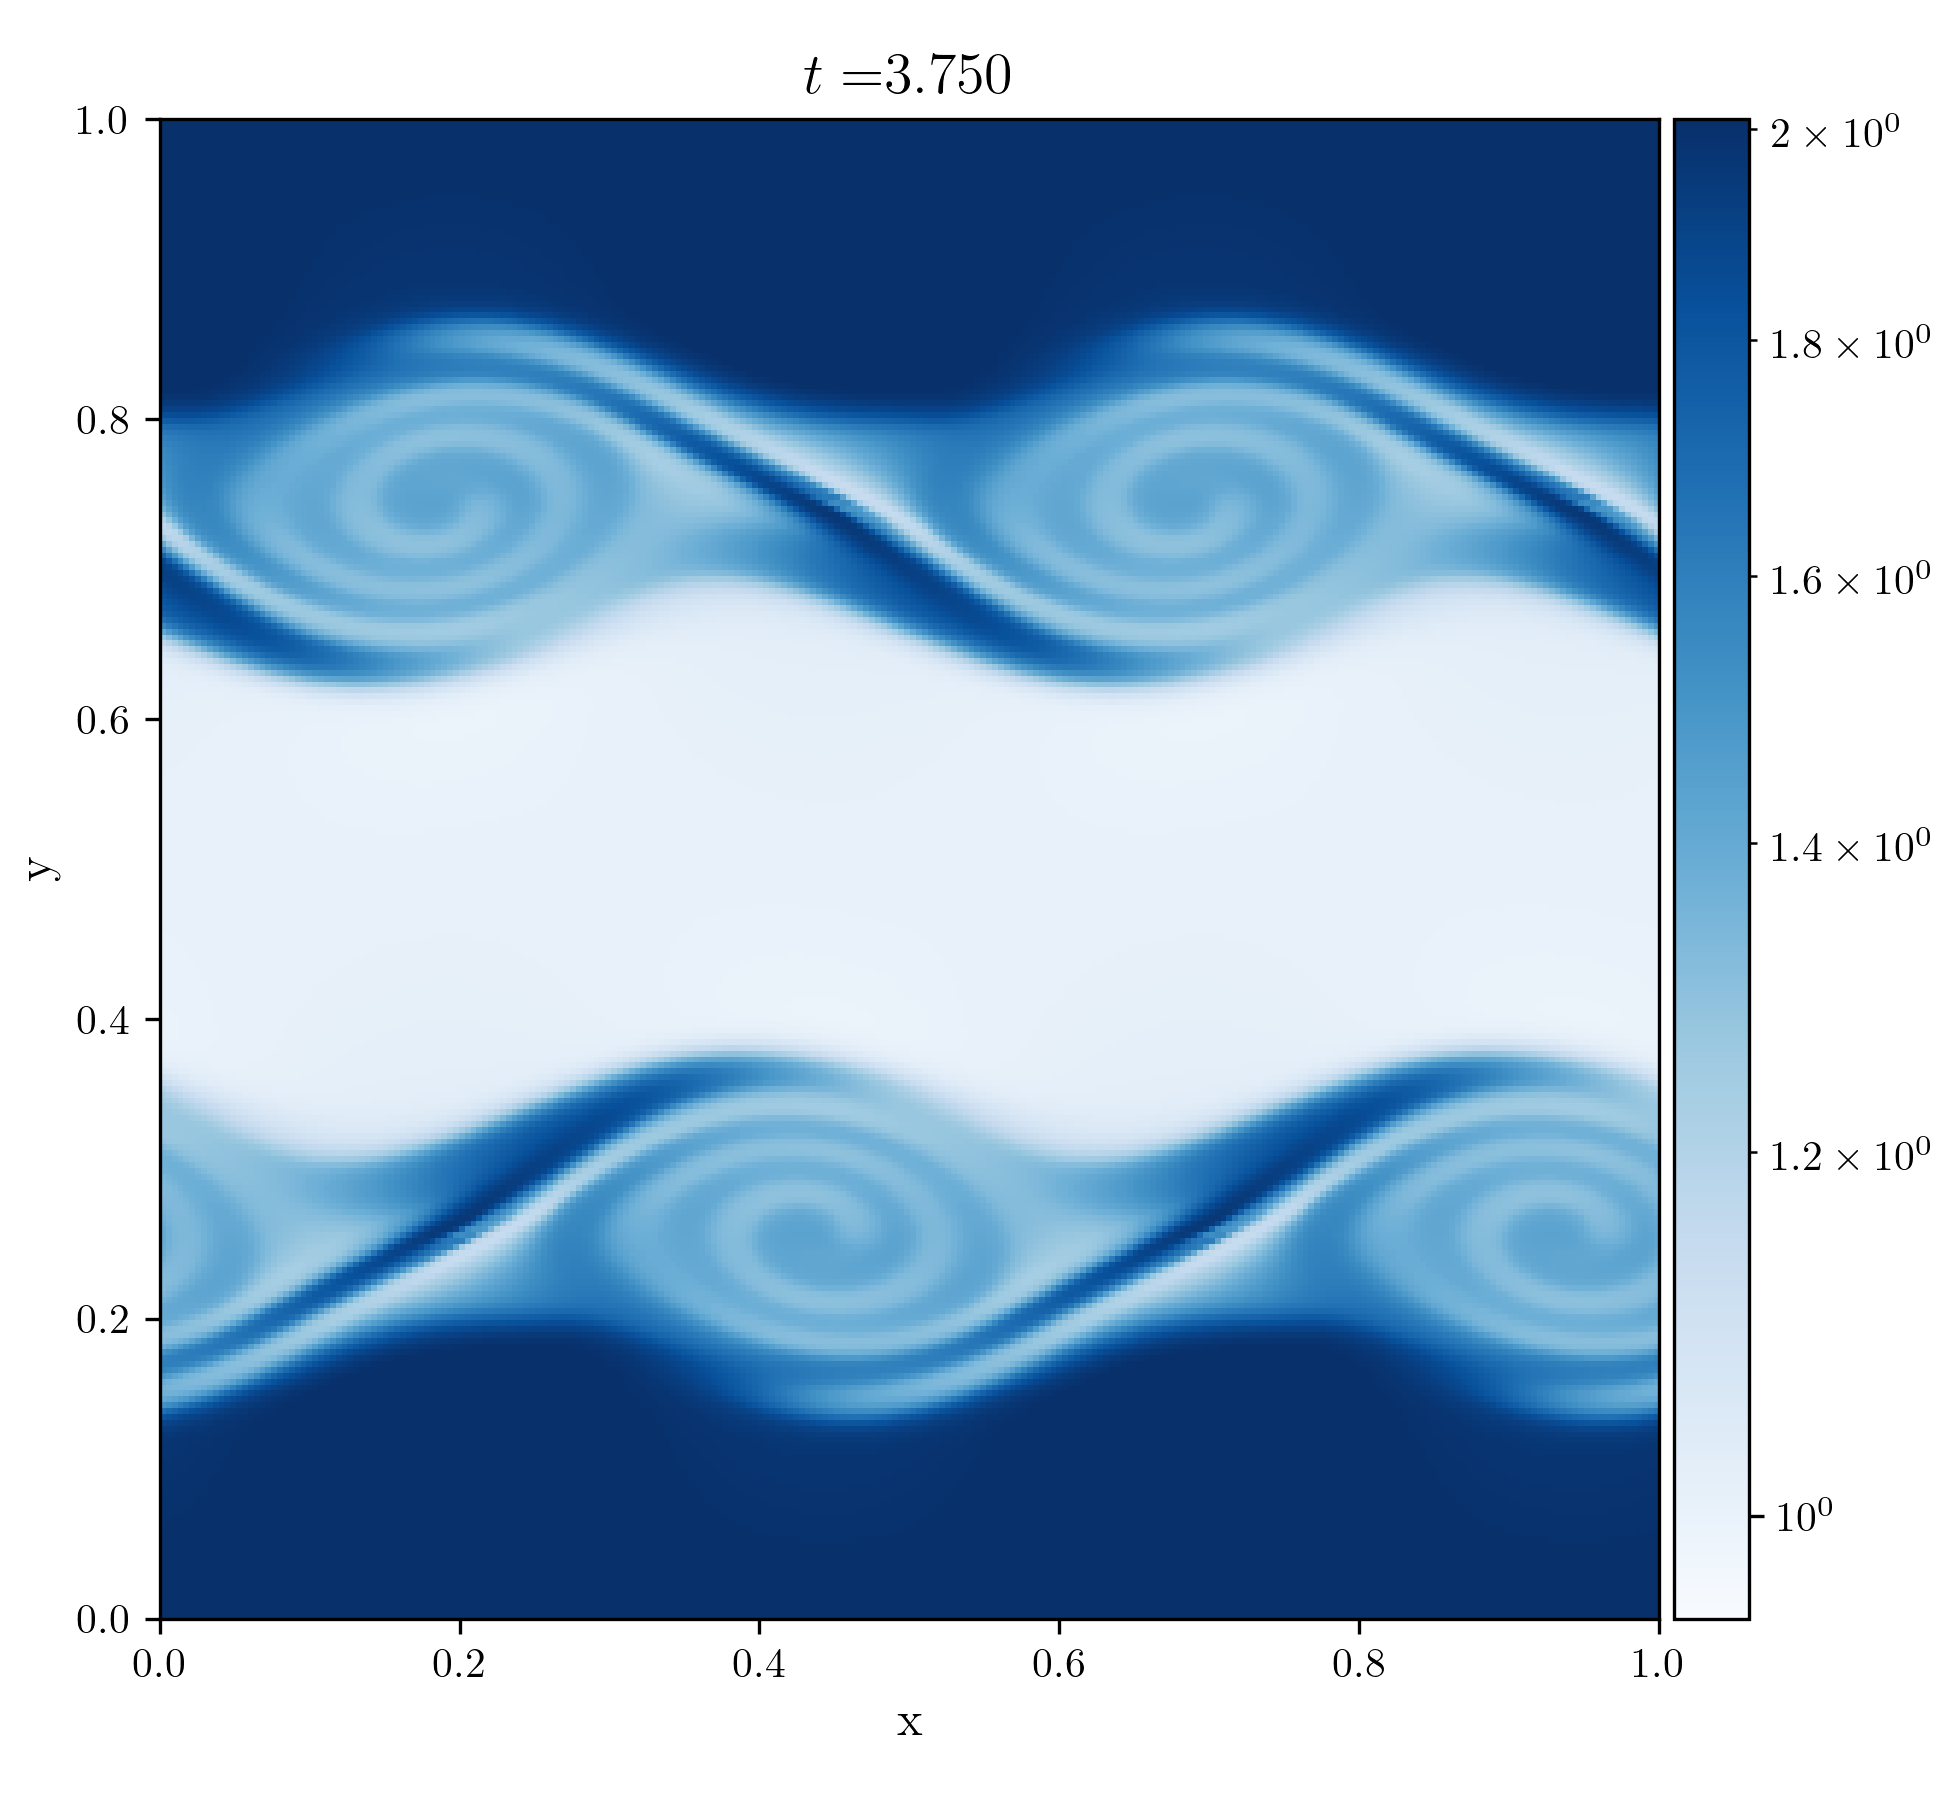
\includegraphics[width=.5\linewidth]{figures/FV/MUSCL-Hancock/kelvin-helmholtz-0750.png}%
\\
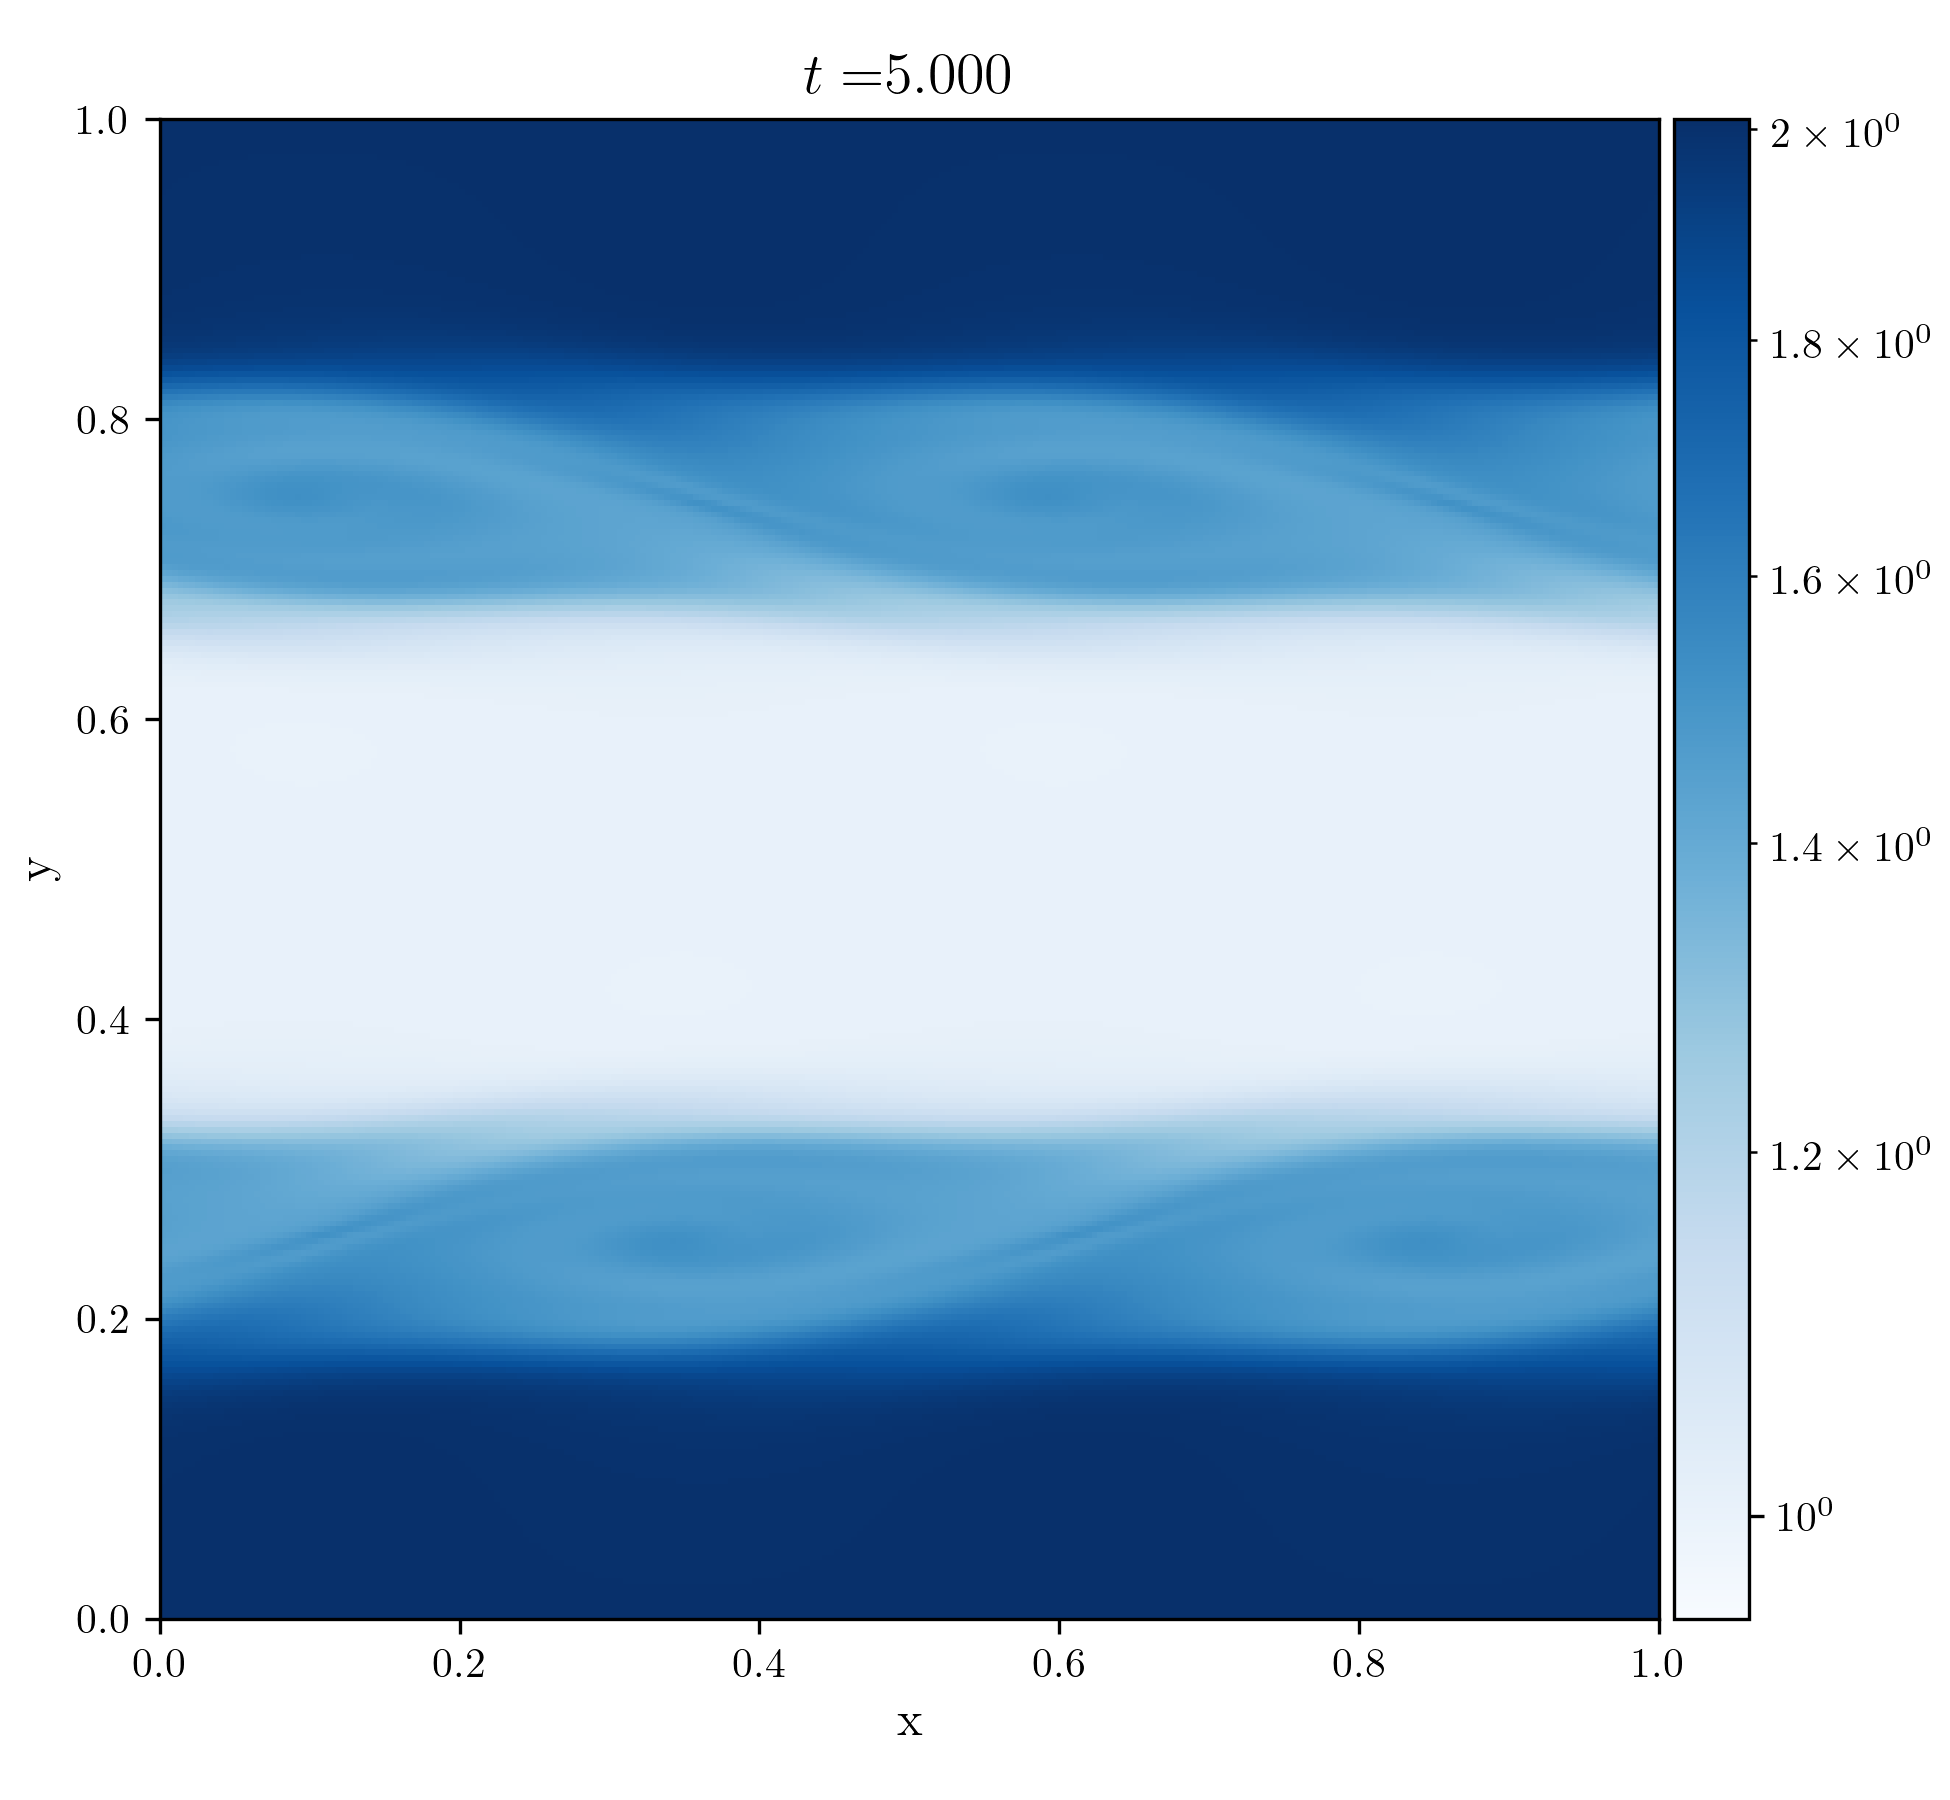
\includegraphics[width=.5\linewidth]{figures/FV/godunov_euler/kelvin-helmholtz-1000.png}%
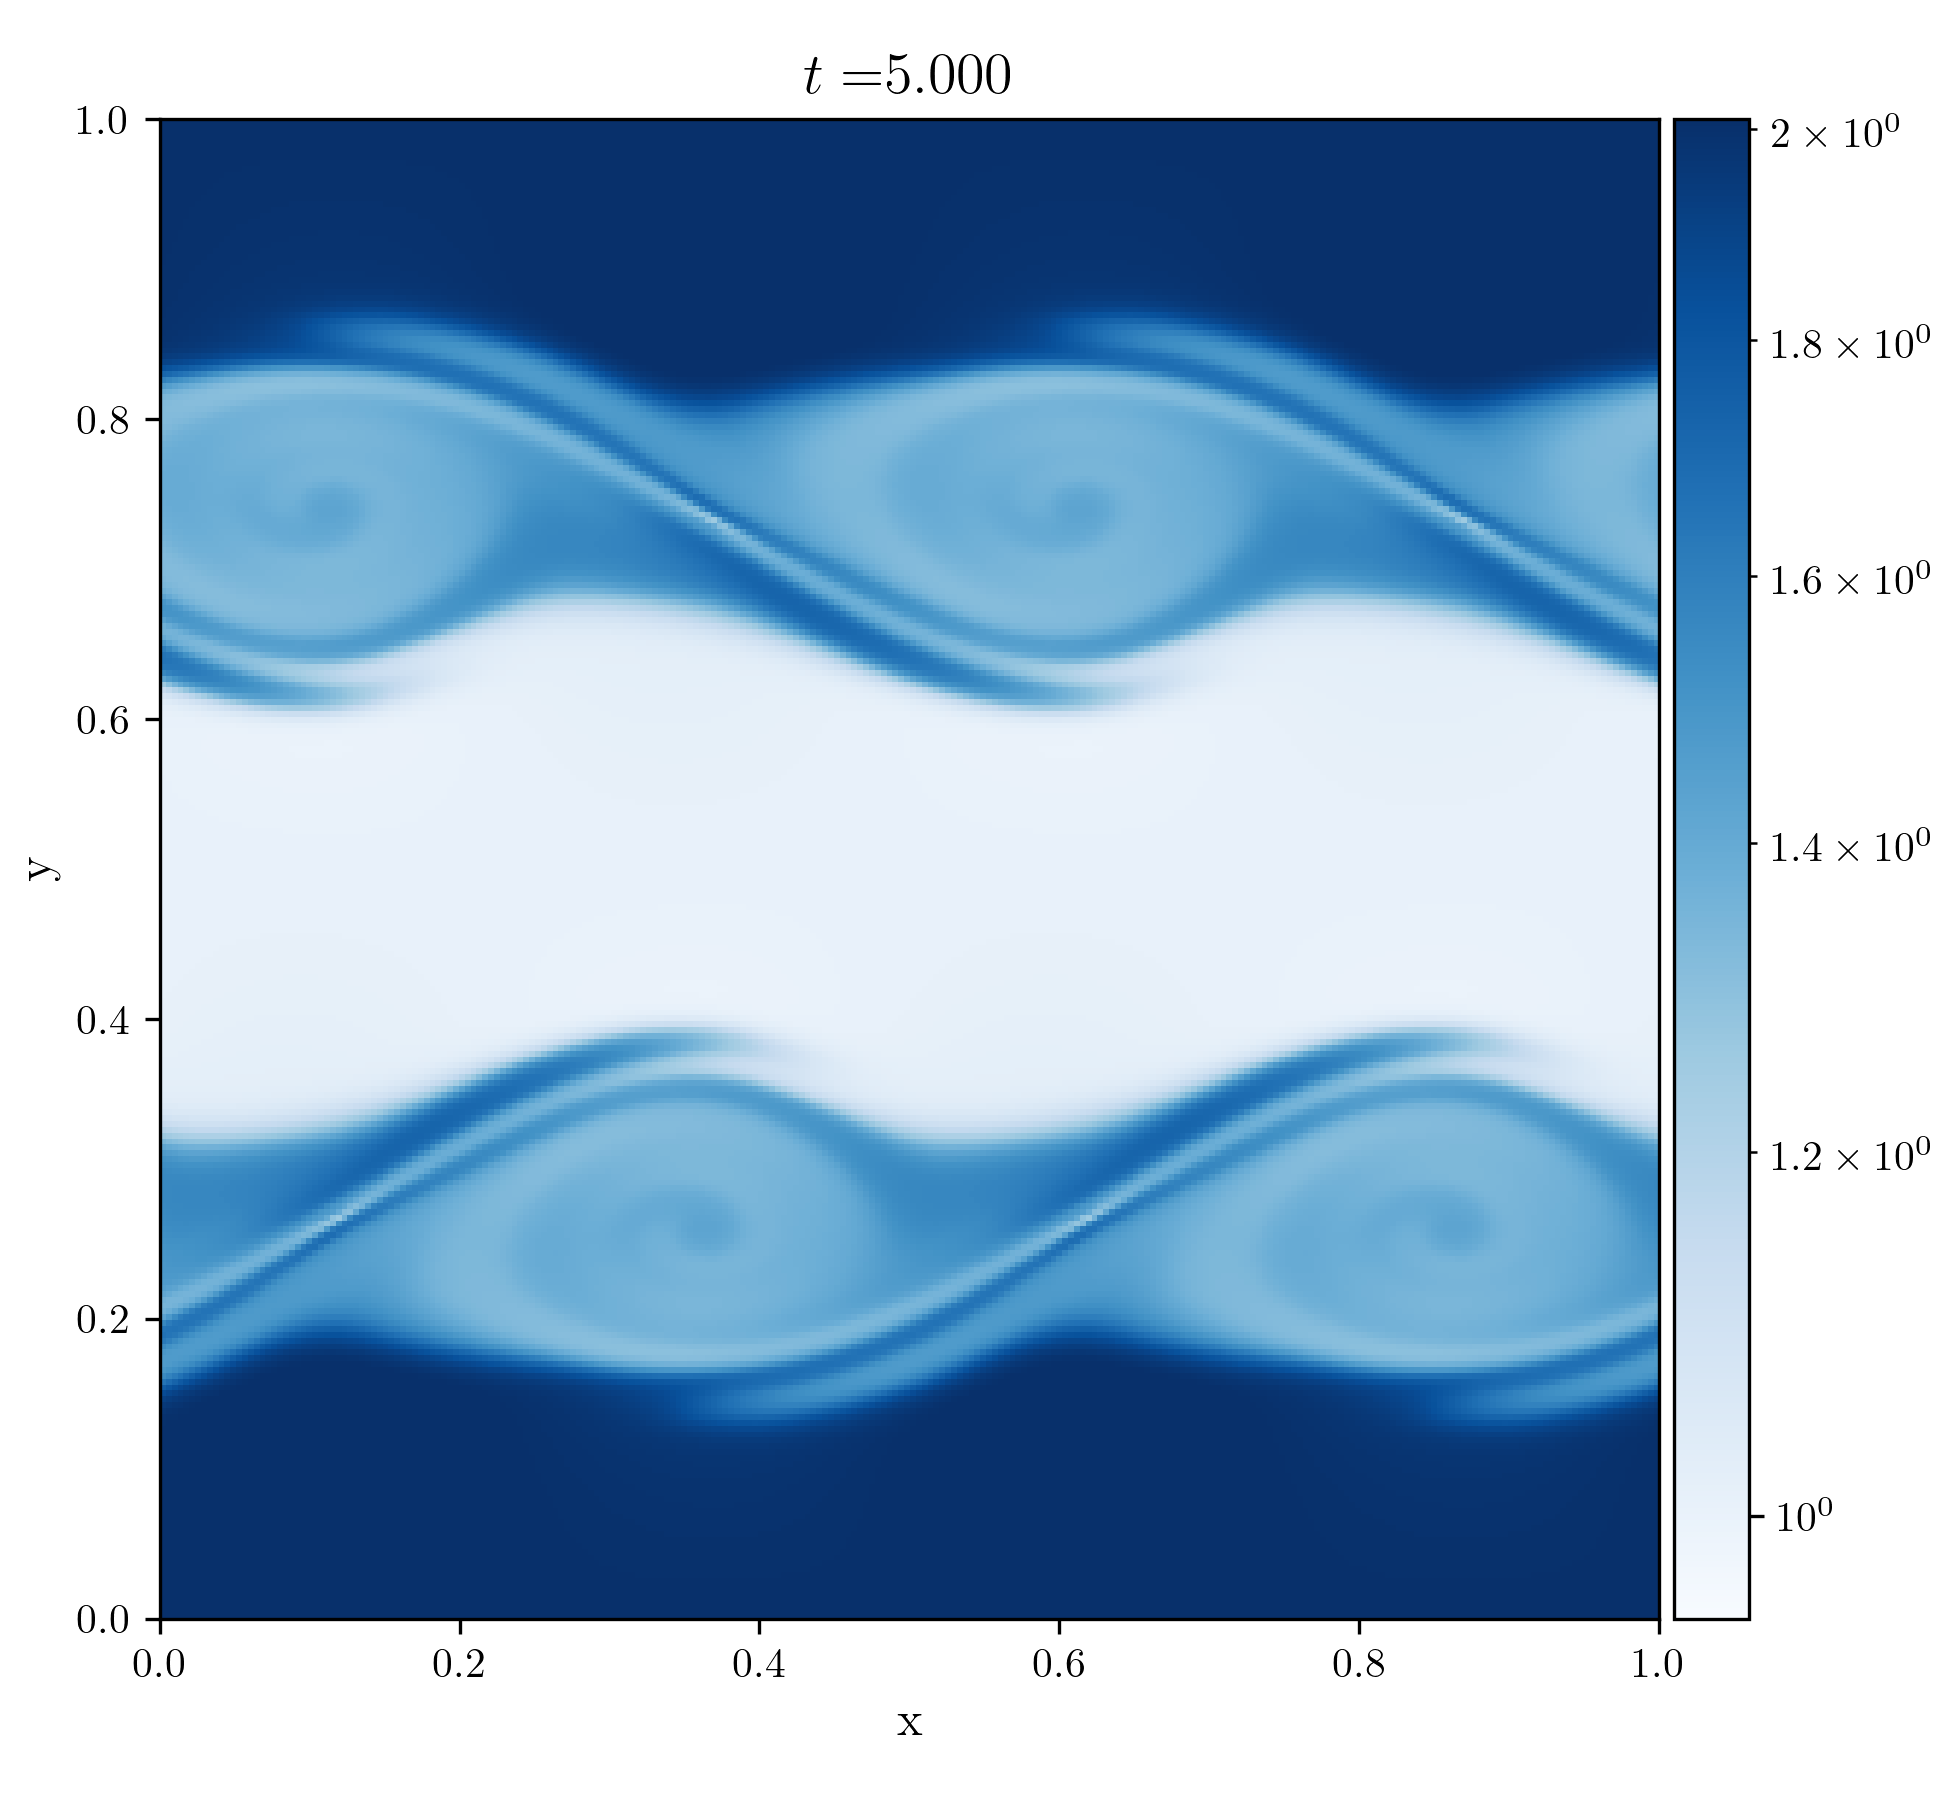
\includegraphics[width=.5\linewidth]{figures/FV/MUSCL-Hancock/kelvin-helmholtz-1000.png}%
\caption[Kelvin-Helmholtz Instability with Godunov's scheme and MUSCL-Hancock 2]{
Density evolution for the Kelvin-Helmholtz instability problem solved with Godunov's method (left)
and the MUSCL-Hancock method (right) at times $t = 2.5, 3.75, 5.$ in arbitrary units.
}
\label{fig:kelvin-helmholtz-2}
\end{figure}













